\RequirePackage{lineno}
\documentclass[review]{elsarticle}
%\linenumbers
\usepackage{verbatim}
\usepackage{graphicx}
\usepackage[utf8]{inputenc}
\usepackage[usenames,dvipsnames,svgnames,table]{xcolor}
\usepackage[breaklinks=true,colorlinks=true,linkcolor=blue,urlcolor=blue,citecolor=blue]{hyperref}
\usepackage{rotating}
\usepackage{graphicx}% Include  files
\usepackage{dcolumn}% Align table columns on decimal point
\usepackage{bm}% bold math
\usepackage{epsfig}
\usepackage{hyperref}
\usepackage{ulem}
\usepackage{appendix}
%\usepackage{iopams}
\usepackage{mwe}
\usepackage{subfig}
\usepackage{lineno}
\expandafter\let\csname equation*\endcsname\relax
\expandafter\let\csname endequation*\endcsname\relax
\usepackage{amsmath}
\usepackage{geometry}
\newgeometry{vmargin={20mm}, hmargin={30mm,22mm}}
%Uncomment next line if AMS fonts required
\usepackage{times}  
%% `Elsevier LaTeX' style
\bibliographystyle{elsarticle-num}
%\usepackage[backend=biber,style=nature]{biblatex}
%\addbibresource{BeautyExp.bib}

%% new commands
\newcommand{\barb}{{\bar{b}}}
\newcommand{\barc}{{\bar{c}}}
\newcommand{\SNN}{$\sqrt{s_{NN}}=$ }
\newcommand{\sqrtsnn}{\ensuremath{\sqrt{s_{NN}}}\xspace}
\newcommand{\raa}{$R_{AA}~$}
\newcommand{\pt}{$p_{T}$}
\newcommand{\npart}{$N_{\rm Part}~$}
\newcommand{\Jpsi}{\ensuremath{J\hspace{-.08em}/\hspace{-.14em}\psi}\xspace} % J/Psi (no mass)
\newcommand{\qqbar}{\ensuremath{q \overline{q}\xspace}\xspace}
\newcommand{\QQbar}{\ensuremath{Q \overline{Q}\xspace}\xspace}
\newcommand{\pp}{{\ensuremath{pp}}\xspace}
\newcommand{\PgU}{\ensuremath{\Upsilon}\xspace}
\newcommand{\PgUa}{\ensuremath{\Upsilon\text{(1S)}}\xspace}
\newcommand{\PgUb}{\ensuremath{\Upsilon\text{(2S)}}\xspace}
\newcommand{\PgUc}{\ensuremath{\Upsilon\text{(3S)}}\xspace}
\newcommand{\fig}[1]{Fig.~\ref{#1}\xspace}
\newcommand{\tab}[1]{Tab.~\ref{#1}\xspace}

\begin{document}
\fontsize{11}{15}
\selectfont

\begin{frontmatter}
  \title{Production of bottomonia states in proton-proton and heavy ion collisions}
  \author[NPD]{Vineet Kumar\corref{mycorrespondingauthor}}
  \cortext[mycorrespondingauthor]{Corresponding author}
  \ead{vineetk@barc.gov.in}
  \author[NPD,HBNI]{Prashant Shukla}
  \author[UOC]{Abhijit Bhattacharyya}
  \address[NPD]{Nuclear Physics Division, Bhabha Atomic Research Centre, Mumbai 400085, India}
  \address[UOC]{Department of Physics, University of Calcutta, 92, A. P. C. Road Kolkata-700009, India}
  \address[HBNI]{Homi Bhabha National Institute, Anushakti Nagar, Mumbai 400094, India}
  \date{\today}
  
  \begin{abstract}
    
    This work reviews the study of bottomonia production in high energy hadronic collisions to investigate
    the fundamental aspects of Quantum Chromodynamics. Emphasis is given to the lessons learnt from the LHC
    data, which are reviewed in a global prospective with the results from the RHIC at lower energies used
    for comparison. The review covers bottomonia production in proton-proton, proton-nucleus and nucleus-nucleus
    collisions and includes discussion of the effects of hot and cold strongly interacting matter.

  \end{abstract}
  
  \begin{keyword}
    Beauty, Quarkonium, Hadron Collision, Heavy-Ion Collision, Quark-Gluon Plasma, LHC, RHIC
  \end{keyword}
  

%\vspace{2pc}
%\noindent{\it Keywords}: Beauty, Quarkonium, Hadron Collision, Heavy-Ion Collision, Quark-Gluon Plasma, LHC, RHIC

  

\maketitle

\tableofcontents


\end{frontmatter}





\section{Introduction}
\label{sec:Introduction}

It is expected that strongly-interacting matter shows qualitatively
new behavior at temperatures and/or densities which are
comparable to or larger than the typical hadronic scale.
It has been argued that under such extreme conditions
deconfinement of quarks and gluons should set in and the 
thermodynamics of strongly-interacting matter could then
be understood in terms of these elementary degrees of freedom.
This new form of matter is called
{\em quark-gluon plasma}~\cite{Shuryak:1980tp,Satz:2011wf}, or QGP.
The existence of such a transition has indeed been demonstrated 
from first principles using Monte Carlo simulations of lattice QCD.
The deconfinement transition and the properties of hot, strongly-interacting 
matter can be studied experimentally in heavy-ion collisions~\cite{Satz:2000bn}. 
A significant part of the extensive experimental heavy-ion
program is dedicated to measuring quarkonium yields since Matsui and Satz
suggested that quarkonium suppression could be a signature of 
deconfinement~\cite{Matsui:1986dk}.

In fact, the observation of anomalous suppression was considered to be
a key signature of deconfinement at SPS energies~\cite{Kluberg:2005yh}.


%However, not all of the observed quarkonium suppression in 
%nucleus-nucleus ($AB$) collisions relative to scaled proton-proton (\pp)
%collisions is due to quark-gluon plasma formation. 
%In fact, quarkonium suppression was also observed in proton-nucleus (pA)
%collisions, so that part of the nucleus-nucleus suppression is due to 
%cold-nuclear-matter effects. Therefore it is necessary to disentangle hot 
%and cold-medium effects. We first discuss cold-nuclear-matter effects
%at different center-of-mass energies. Then we discuss what is known 
%about the properties of heavy \QQbar states in hot, deconfined media. 
%Finally, we review recent experimental results on quarkonium production from
%\pp, pA and AA collisions at the SPS, RHIC and LHC.




\section{Bottomonia production mechanism in p-p collisions}
\label{sec:Bottomonia_pp_th}


In general one can subdivide the quarkonia production process into two major parts

\begin{enumerate}
\item Production of a heavy quark pair in hard collisions.
\item Formation of quarkonia out of the two heavy quarks.
\end{enumerate}

First process can be calculated by the perturbative QCD calculations while the 
formation of quarkonia out of the two heavy quarks is a non perturbative process 
and require some effective theories for modelling. 

\subsection{Production of a heavy quark pair in hard collisions}
\label{subsec:HeavyQuarkProd}
Due to the high mass of the heavy quarks (m$_{\rm c}\,\sim$ 1.3 GeV/c$^2$, m$_{\rm b}\,\sim$ 4.7 GeV/c$^2$), 
they can be produced only during the first phase of a collision.
Only at that time the elementary collisions with sufficiently high momentum 
transfers (to create such high masses) takes place. For this reason the heavy quark production
is a hard process that can be treated perturbatively.
The hadronic cross section in $pp$ collisions can
be written as
\begin{eqnarray}
\sigma_{pp}(s,m^2) & = & \sum_{i,j = q, \overline q, g} 
\int dx_1 \, dx_2 \, 
f_i^p (x_1,\mu_F^2) \,
f_j^p(x_2,\mu_F^2) \, \widehat{\sigma}_{ij}(s,m^2,\mu_F^2,\mu_R^2)
\label{sigpp}
\end{eqnarray}
where $x_1$ and $x_2$ are the fractional momenta carried by the colliding
partons and $f_i^p$ are the proton parton densities.
The total partonic cross section has been completely calculated up to NLO
\cite{Nason:1987xz,Nason:1989zy}. The partonic cross section is given by
\begin{eqnarray}
\widehat{\sigma}_{ij}(s,m,\mu_F^2,\mu_R^2) & = & 
\frac{\alpha_s^2(\mu_R^2)}{m^2}
\left\{ f^{(0,0)}_{ij}(\rho) \right. \nonumber \\
 & + & \left. 4\pi \alpha_s(\mu_R^2) \left[f^{(1,0)}_{ij}(\rho) + 
f^{(1,1)}_{ij}(\rho)\ln\bigg(\frac{\mu_F^2}{m^2} \bigg) \right] 
+ {\cal O}(\alpha_s^2) \right\}
\,\, 
\label{sigpart}
\end{eqnarray}
where $\rho = 4m^2/s$ and 
$f_{ij}^{(k,l)}$ are the scaling functions to NLO \cite{Nason:1987xz,Nason:1989zy}. 
At small $\rho$, the ${\cal O}(\alpha_s^2)$ and ${\cal O}(\alpha_s^3)$
$q \overline q$ and the ${\cal O}(\alpha_s^2)$ $gg$ scaling functions 
become small while the ${\cal O}(\alpha_s^3)$ $gg$ and $qg$ scaling functions
plateau at finite values.  Thus, at collider energies, the total cross sections
are primarily dependent on the small $x$ parton densities and phase space.
The total cross section does not depend on any kinematic variables, 
only on the quark mass, $m$, and the renormalization and factorization scales with central
value $\mu_{R,F} =\mu_0 = m$.

\subsection{Formation of quarkonia out of the two heavy quarks}
\label{subsec:QuarkoniaProdFromHeavyQuarks}

The nonperturbative evolution of the $Q\bar Q$ pair into a quarkonium
has been discussed extensively in terms of models and in terms of the
language of effective theories of QCD
\cite{Bodwin:1994jh,Brambilla:2004wf}. Different
treatments of this evolution have led to various theoretical models for
inclusive quarkonium production. Most notable among these are the color-singlet
model (CSM), the color-evaporation model (CEM) and the non-relativistic QCD
(NRQCD) factorization approach. In this review we will mainly discuss the NRQCD 
approach, as theoretically, it is the most modern and acceptable one. However,
we will touch upon CSM and CEM briefly. 


\subsubsection{The color singlet model : }
%\label{prod_sec:CSM}

The CSM was first proposed shortly after the discovery of the 
$\Jpsi$~\cite{Einhorn:1975ua,Ellis:1976fj,Carlson:1976cd,Berger:1980ni}.
In this model, it is assumed that the $Q\bar Q$ pair that evolves into
the quarkonium is in a color-singlet state and that it has the same spin
and angular-momentum quantum numbers as the quarkonium. In the CSM, the
production rate for each quarkonium state is related to the absolute
values of the color-singlet $Q\bar Q$ wave function and its derivatives,
evaluated at zero $Q\bar Q$ separation. These quantities can be
extracted by comparing theoretical expressions for quarkonium decay
rates in the CSM with experimental measurements. Once this extraction
has been carried out, the CSM has no free parameters. The CSM was
successful in predicting quarkonium production rates at relatively low
energy \cite{Schuler:1994hy}. Recently, it has been found that, at high
energies, very large corrections to the CSM appear at next-to-leading
order (NLO) and next-to-next-to-leading order (NNLO) in $\alpha_s$
\cite{Artoisenet:2007xi,Campbell:2007ws,Artoisenet:2008fc}.
Consequently, the possibility that the CSM might embody an important 
production mechanism at high energies has re-emerged. 
However, given the very large corrections at
NLO and NNLO, it is not clear that the perturbative expansion in
$\alpha_s$ is convergent. 
%Furthermore, in the production and decay of
%$P$-wave and higher-orbital-angular-momentum quarkonium states, the CSM
%is known to be inconsistent because it leads to uncanceled infrared
%divergences. (See Ref.~\cite{Brambilla:2004wf} and references therein.)
The NRQCD factorization approach encompasses
the color-singlet model, but goes beyond it.

\subsubsection{The color evaporation model:}  
\label{prod_sec:CEM}

The CEM~\cite{Fritzsch:1977ay,Amundson:1995em,Amundson:1996qr}
is motivated by the principle of quark-hadron duality. In the CEM, it
is assumed that every produced $\QQbar$ pair evolves into a quarkonium
if it has an invariant mass that is less than the threshold for
producing a pair of open-flavor heavy mesons. It is further assumed that
the nonperturbative probability for the $\QQbar$ pair to evolve into a
quarkonium state $H$ is given by a constant $F_H$ that is
energy-momentum and process independent. Once $F_H$ has been fixed by
comparison with the measured total cross section for the production of
the quarkonium $H$, the CEM can predict, with no additional free
parameters, the momentum distribution of the quarkonium production rate. The
CEM predictions provide good descriptions of the CDF data for $\Jpsi$,
$\psi(2S)$, and $\chi_{c}$ production at $\sqrt{s}=1.8$~TeV
\cite{Amundson:1996qr}. 

%In Ref.~\cite{Bodwin:2005hm}, the CEM
%predictions are fit to the CDF data for $J/\psi$, $\psi(2S)$, and
%$\chi_{cJ}$ production at $\sqrt{s}=1.8$~TeV \cite{Abe:1997yz}. The
%quality of these fits is generally poor, with $\chi^2/\hbox{d.o.f.}$ for
%the $J/\psi$ fits of about $7$--$8$ without initial-state $k_T$ smearing and
%$2$--$4.5$ with initial-state $k_T$ smearing. In contrast, the NRQCD
%factorization approach, which we are about to describe, yields fits to
%the CDF $J/\psi$ data with $\chi^2/\hbox{d.o.f.}$ of about $1$.

The heavy quark production cross section are calculated to NLO in pQCD  
using the CT10 parton densities \cite{Lai:2010vv}. The mass and scale parameters used 
for open and hidden heavy flavor production are obtained by fitting the energy dependence 
of open heavy flavor production to the measured total cross sections~\cite{Nelson:2012bc,Nelson:Future}.
Those obtained for open charm are $m_c = 1.27 \pm 0.09$~GeV,
$\mu_F/m_{T\,c} = 2.10 ^{+2.55}_{-0.85}$, and $\mu_R/m_{T\, c} = 1.60 ^{+0.11}_{-0.12}$~\cite{Nelson:2012bc}. 
The botttom quark mass and scale parameters are $m_b = 4.65 \pm 0.09$ GeV,
$\mu_F/m_{T\, b} = 1.40^{+0.75}_{-0.47}$, and $\mu_R/m_{T\, b} = 1.10^{+0.26}_{-0.19}$~\cite{Nelson:Future}.
The quarkonium production cross sections are calculated in the color evaporation model with
normalizations determined from fitting the scale parameter to the shape of the energy-dependent
cross sections~\cite{Nelson:2012bc,Nelson:Future}. The resulting uncertainty bands are smaller 
than those obtained with the fiducial parameters used in Ref.~\cite{Cacciari:2005rk}.
We note that the new results are within the uncertainties of those Ref.~\cite{Cacciari:2005rk}.  
Indeed, the charm cross sections reported at the LHC agree
better with the new values of the mass and scale than the central value of $m_c = 1.5$ GeV,
$\mu_F/m_T = \mu_R/m_T = 1$. The central EPS09 NLO parameter set~\cite{Eskola:2009uj} is used to 
calculate the modifications of the parton distribution functions (nPDF) in 
Pb+Pb collisions, referred as cold nuclear matter (CNM) effects. The CNM uncertainty is 
calculated by adding the EPS09 NLO uncertainties in quadrature.%}
The production cross sections for heavy flavor and quarkonia at $\sqrt{s_{_{_{NN}}}}$ = 2.76 
TeV \cite{Kumar:2012qx} are given in Table~\ref{NLOcros}.  The yields in a minimum bias 
Pb+Pb event is obtained from the per nucleon cross
section, $\sigma_{\rm PbPb}$, in Table~\ref{NLOcros}, as
\begin{eqnarray}
N = {A^2 \sigma_{\rm PbPb} \over  
\sigma_{\rm PbPb}^{\rm tot}} \, \, .
\end{eqnarray}
 At 2.76 TeV, the total Pb+Pb cross section, $\sigma_{\rm PbPb}^{\rm tot}$, 
is 7.65 b \cite{Chatrchyan:2011sx}.


\begin{table}
\caption[]{Heavy quark and quarkonia production  cross sections at
$\sqrt{s_{_{_{NN}}}}= 2.76$ TeV. The cross sections are given per nucleon pair while
$N^{\rm PbPb}$ gives the initial number of heavy quark pair/quarkonia per Pb+Pb event.}
\label{NLOcros}
\begin{tabular}{l|l|l|l|l} 
\hline 
\hline
             & $ c \overline c$            &$\Jpsi$                      & $ b \overline b$                    & $\Upsilon$   \\              
\hline
$\sigma_{pp}$ & $4.11^{+2.69}_{-2.50}$ mb    & $21.6^{+10.6}_{-10.4}~\mu$b   & $110.5^{+15.1}_{-14.2}~\mu$b            & $0.22^{+0.07}_{-0.06}~\mu$b  \\


$\sigma_{\rm PbPb}$ & $3.21^{+2.1}_{-1.95}$ mb    &16.83$^{+8.26}_{-8.10}~\mu$b    & $100.5^{+13.7}_{-12.9}~\mu$b             & 0.199$^{+0.063}_{-0.054}~\mu$b  \\



$N^{\rm PbPb}$     & $18.12^{+12}_{-11}$       & $0.0952^{+0.047}_{-0.046}$         & $0.57^{+0.08}_{-0.07}$                          & $0.001123^{+0.0004}_{-0.0003}$       \\

\hline
\hline
\end{tabular}
\end{table}






\subsubsection{The NRQCD factorization approach:}


Quantum Chromodynamics (QCD) describes the strong interaction among the
quarks and gluons via perturbative calculations utilising its property called asymptotic freedom.
On the other hand, these quarks and gluons are confined inside hadrons which are the colour singlet states.
Confinement is a purely non-perturbative phenomenon which is not very well understood yet. 
The study of quarkonia ($Q\bar{Q}$) serves as an effective 
tool to look at  both of these perturbative and non-perturbative aspects of QCD.
The quarkonia states differ from most other hadrons due to the small velocity, $v$ of the massive
constituents and thus can be treated using non-relativistic formalism~\cite{Povh:1995mua,Ikhdair:2005jf}. 
In a simple picture, one can think of a quarkonium as a heavy quark pair ($Q\bar{Q}$) bound
in a colour singlet state by some effective potential interaction, where the constituents are 
separated by distances much smaller than $1/\Lambda_{\rm QCD}$ where $\Lambda_{\rm QCD}$
is the QCD scale. This interaction gets screened 
in the presence of a deconfined medium like Quark Gluon Plasma (QGP), causing 
the bound state to melt away and thus the quarkonia yields are suppressed in the 
heavy ion collisions. This makes quarkonia an important probe of QGP. However cold nuclear matter 
effects such as modification of parton distribution functions of nucleons inside nucleus also 
affect their yields.
There have been immense experimental~\cite{Sirunyan:2017isk,Sirunyan:2018nsz,Acharya:2019iur,Acharya:2018mni}
and theoretical works~\cite{Strickland:2011mw,Song:2011nu,Kumar:2014kfa,Kumar:2019xdj} on
quarkonia modifications in PbPb collisions for which understanding of quarkonia
production in pp collisions is an important prerequisite.

The massive quarks (with $m_c\sim 1.6$ GeV/$c^2$, $m_b\sim 4.5$ GeV/$c^2$) are produced
in initial stages in hadronic collision with high momentum transfer and thus
can be treated perturbatively~\cite{Nason:1989zy}. The emergence of quarkonia
out of the two massive quarks, on the other hand can only be described non-perturbatively using different
models~\cite{Bodwin:1994jh,Brambilla:2014jmp}.
The Colour Singlet Model (CSM)~\cite{Einhorn:1975ua,Berger:1980ni},
Colour Evaporation Model (CEM)~\cite{Fritzsch:1977ay,Amundson:1995em}, the Fragmentation Scheme and 
the NRQCD factorisation formalism are some of the well established models for quarkonia production.
In the framework of CSM, the $Q\bar{Q}$ pair, eventually evolving into the quarkonium,
is assumed to be in Colour Singlet (CS) state and that has spin and 
angular momentum same as that of quarkonium.
Apart from comprising of the CSM, the NRQCD factorisation approach incorporates 
the Colour Octet (CO) states as well.

In the formalism of the NRQCD factorisation approach, the evolution probability of $Q\bar{Q}$
pair into a state of quarkonium is expressed as matrix elements of NRQCD operators expanded
in terms of heavy quark velocity $v$ (for $v\ll$1)~\cite{Bodwin:1994jh}.
%The NRQCD formalism based on an effective field 
%theory framework, separates the short distance annihilation scale of heavy 
%quarkonium states from long distance ones corresponding to quarkonium structure.
The factorisation formulae were then used to calculate production cross-sections
and decay rates of quarkonia states.
%S-wave states at Next to leading order (NLO) and of P-wave
%states at Leading order (LO).
The full structure of the $Q\bar{Q}$ Fock space
is considered and spanned by $n$=$^{2s+1}L_J^{[a]}$ state where $s$
is the spin, $L$ is the orbital angular momentum, $J$ is the total angular momentum
and $a$ (colour multiplicity) = 1 for CS and 8 for CO states. 
The produced CO states of $Q\bar{Q}$ pair at short distances emerge as 
CS quarkonia by emitting soft gluons non-perturbatively.
%In case of S-wave quarkonia, the CSM is retrieved in the limit of $v\rightarrow$0.
The short distance cross-sections are obtained theoretically
using methods of perturbative QCD (pQCD). The long distance matrix elements
(LDME) that correspond to the probability of 
$Q\bar{Q}$ pair to emerge as quarkonium are extracted by fitting the measured cross-section
data.

There have been several works on bottomonia production based on
NRQCD formalism. In Ref.~\cite{Domenech:1999qg}, a Monte Carlo framework has first
been employed with CO mechanism for inclusive bottomonia production and few
NRQCD CO matrix elements for $\Upsilon$(1S) have been extracted at the Tevatron energy. 
The study has been extended to the whole $\Upsilon$(nS) family in Ref.~\cite{Domenech:2000ri}
to find CO matrix elements using CDF measurements at Tevatron.
In Ref.~\cite{Brateen:PRD2001} the CO matrix elements are obtained for $\Upsilon$(nS) family
and the feed downs from $\chi_{b}$(1P) and $\chi_{b}$(2P) to $\Upsilon$(1S) have been 
considered.
In Ref.~\cite{Gong:2010bk}, the $\Upsilon$ production has been obtained via
S-wave CO states calculated at Next to Leading Order (NLO). The LDMEs are obtained
by fitting the Tevatron data. The ratios of NLO to LO total cross-sections
have been obtained at Tevatron and LHC energies. Polarisation of inclusive
$\Upsilon$ has been obtained albeit with large uncertainties.
In Ref.~\cite{Sharma:2012dy} both CS and CO states along with
feed down contributions from higher states have been considered to study the
quarkonia yields for RHIC and LHC energies.
Using Collins-Soper-Sterman (CSS) formalism, an extension of the NRQCD prediction
has been carried forward for heavy quarkonium production
at low $p_T$ by considering soft gluon resummation at all orders in Ref.~\cite{Sun:2012vc}.

Both production and polarisation of $\Upsilon$(nS) at NLO have been discussed in 
Ref.~\cite{Gong:2013qka} within the framework of NRQCD. The CO matrix elements are obtained
by fitting with experimental data. The study is updated in Ref.~\cite{Feng:2015wka} by considering
feed down from $\chi_{bJ}$(mP) states in $\Upsilon$(nS) production. The yields and
polarisations of $\Upsilon$(nS) measured at Tevatron and LHC are well explained by this work.
The NLO study in Ref.~\cite{Han:2014kxa} describes the yields and polarisations of
$\Upsilon$(nS) at LHC which includes feed down contributions from
higher states. In Ref.~\cite{Yu:2017pot}, production cross-section for $\Upsilon$(nS),
$\chi_{bJ}$, $\eta_b$ and $h_b$ have been calculated using NRQCD, as produced in hard
photo production and fragmentation processes at LHC energies. 

A LO NRQCD analyis is useful as it is straightforward and unique and once the parameters are
obtained by fitting over large datasets it has excellent predictability power for unknown cross
sections. The short distance QCD cross-sections calculation techniques at NLO are not unique.
Moreover the different components of pQCD NLO cross sections are not available in
public domain. Many NLO analysis do not include the feed down contribution from the higher
states. It is shown that there is a large difference amoung the LDMEs obtained by different
analysis at NLO. In this paper, the LO NRQCD calculations for the differential production
cross-sections of $\Upsilon$ states in p+p collisions have been presented.
The NRQCD formalism is described
briefly in Section~\ref{sec:formalism}. 
A large set of data from Tevatron~\cite{Acosta:2001gv} and
LHC~\cite{LHCb:2012aa,Khachatryan:2015qpa,Aad:2012dlq,Chatrchyan:2013yna,Sirunyan:2017qdw} 
is used to extract the LDMEs required for the $\Upsilon$ production and then results are
presented in Section~\ref{sec:results}. A comparison of the obtained LDMEs with the
previous NRQCD studies both at LO and NLO has been made. The summary 
of our findings are discussed in Section~\ref{sec:summary}. An updated QCD LO study on the
bottomonia hadroproduction is useful as it provides a reference for comparison
with NLO calculations. 




\begin{table*}
  \centering
  \caption{Necessary and pertinent branching fractions for bottomonia family~\cite{Han:2014kxa,Zyla:2020zbs}.}
  \footnotesize
  %\begin{tabular}{ccccccccc}
  \begin{tabular*}{\textwidth}{@{\extracolsep{\fill}}lrrrrrrrrl@{}}
    \hline
    \hline
    & & & & & & & & &\\
    Meson from & & & & & Meson to & & & & \\ \\
    \hline 
    &$\Upsilon$(3S) &$\chi_{b0}$(2P) &$\chi_{b1}$(2P) &$\chi_{b2}$(2P) &$\Upsilon$(2S) &$\chi_{b0}$(1P) &$\chi_{b1}$(1P) &$\chi_{b2}$(1P) &$\Upsilon$(1S)\\
    %& & (GeV) & $({\rm GeV^3})$ & $({\rm GeV^3})$ & $({\rm GeV^3})$ & \\ \\
    \hline
    \hline \\
    $\chi_{b0}$(3P) &0.005 & & & &0.002 & & & & 0.002 \\ \\
    $\chi_{b1}$(3P) &0.104 & & & &0.037 & & & & 0.038 \\ \\
    $\chi_{b2}$(3P) &0.061 & & & &0.019 & & & & 0.019 \\ \\
    $\Upsilon$(3S) & & 0.131 &0.126 & 0.059 & 0.199 & 0.003 & 0.0017 & 0.019 & 0.066 \\ \\
    $\chi_{b0}$(2P) & & & & &0.014 & & & & 0.004 \\ \\
    $\chi_{b1}$(2P) & & & & &0.199 & & & & 0.092 \\ \\
    $\chi_{b2}$(2P) & & & & &0.106 & & & & 0.070 \\ \\
    $\Upsilon$(2S) & & & & & & 0.038 & 0.0715 & 0.069 & 0.260 \\ \\
    $\chi_{b0}$(1P) & & & & & & & & & 0.019 \\ \\
    $\chi_{b1}$(1P) & & & & & & & & & 0.352 \\ \\
    $\chi_{b2}$(1P) & & & & & & & & & 0.180 \\ \\
    \hline
    \hline
  \end{tabular*}
  \label{BRUpsilon}
\end{table*}
\normalsize
%\par 
\begin{table*}
  \centering
  \caption{CS and CO elements for $\Upsilon$ family, obtained theoretically/extracted using experimental data~\cite{Sharma:2012dy,Feng:2015wka}.}
  \footnotesize
  %\begin{tabular}{ccc}
  \begin{tabular*}{\textwidth}{@{\extracolsep{\fill}}lrrrrl@{}}
    \hline
    \hline
    & & \\ 
    Direct Contributions & Feed down contributions & Feed down contributions \\
    & from higher s-wave states & from higher p-wave states \\ \\
    \hline 
    & & \\
    $M_L(b\bar{b}([^3S_1]_1)\rightarrow\Upsilon(3S))$ & $M_L(b\bar{b}([^3S_1]_1)\rightarrow\Upsilon(3S,2S))$
    & $M_L(b\bar{b}([^3P_0]_1)\rightarrow\chi_{b0}(1P))$ \\
    =4.3 ${\rm GeV^3}$ & =4.3, 4.5 ${\rm GeV^3}$ & =0.100$m_b^2$ ${\rm GeV^3}$ \\ \\
    
    $M_L(b\bar{b}([^3S_1]_1)\rightarrow\Upsilon(2S))$ & $M_L(b\bar{b}([^3S_1]_8)\rightarrow\Upsilon(3S,2S))$
    & $M_L(b\bar{b}([^3S_1]_8)\rightarrow\chi_{b0}(1P))$ \\
    =4.5 ${\rm GeV^3}$ & & =0.0094 ${\rm GeV^3}$ \\ \\
    
    $M_L(b\bar{b}([^3S_1]_1)\rightarrow\Upsilon(1S))$ & $M_L(b\bar{b}([^1S_0]_8)\rightarrow\Upsilon(3S,2S))$
    & $M_L(b\bar{b}([^3P_0]_1)\rightarrow\chi_{b0}(2P))$ \\
    =10.9 ${\rm GeV^3}$ &  & =0.100$m_b^2$ ${\rm GeV^3}$ \\ \\
    
    $M_L(b\bar{b}([^3S_1]_8)\rightarrow\Upsilon(nS))$ & $M_L(b\bar{b}([^3P_0]_8)\rightarrow\Upsilon(3S,2S))$
    & $M_L(b\bar{b}([^3S_1]_8)\rightarrow\chi_{b0}(2P))$ \\
    &  & =0.0109 ${\rm GeV^3}$ \\ \\
    
    $M_L(b\bar{b}([^1S_0]_8)\rightarrow\Upsilon(nS))$ & $M_L(b\bar{b}([^3P_1]_8)\rightarrow\Upsilon(3S,2S))$ &$M_L(b\bar{b}([^3P_0]_1)\rightarrow\chi_{b0}(3P))$ \\
    & =3$M_L(b\bar{b}([^3P_0]_8)\rightarrow\Upsilon(3S,2S))$ &=0.100$m_b^2$ ${\rm GeV^3}$  \\ \\
    
    $M_L(b\bar{b}([^3P_0]_8)\rightarrow\Upsilon(nS))$ & $M_L(b\bar{b}([^3P_2]_8)\rightarrow\Upsilon(3S,2S))$ &$M_L(b\bar{b}([^3S_1]_8)\rightarrow\chi_{b0}(3P))$ \\
    & =5$M_L(b\bar{b}([^3P_0]_8)\rightarrow\Upsilon(3S,2S))$ &=0.0069 ${\rm GeV^3}$ \\ \\
    
    $M_L(b\bar{b}([^3P_1]_8)\rightarrow\Upsilon(nS))$ & & \\
    3$M_L(b\bar{b}([^3P_0]_8)\rightarrow\Upsilon(nS))$ & &  \\ \\
    
    $M_L(b\bar{b}([^3P_2]_8)\rightarrow\Upsilon(nS))$ & & \\
    5$M_L(b\bar{b}([^3P_0]_8)\rightarrow\Upsilon(nS))$ & &  \\ \\
    \hline
    \hline
  \end{tabular*}
  \label{CSCO}
\end{table*}
\normalsize

\paragraph{Bottomonia production in p$+$p collisions}
\label{sec:formalism}
In order to study heavy quarkonium yield, the NRQCD framework serves as an
efficient theoretical tool. The processes that govern the differential
production of heavy mesons like bottomonium, as functions of $p_T$ are mostly
2$\rightarrow$2 operations. These processes can be denoted generically by 
$a+b\rightarrow \Upsilon +X$, where $a$ and $b$ are the incident light partons,
$\Upsilon$ is the heavy meson and $X$ is final state light parton.
The double differential cross-section as a function of $p_T$ and rapidity ($y$) of 
the heavy meson can be written as~\cite{Kumar:2016ojy},
\begin{eqnarray}
  \nonumber
  \frac{d^2\sigma^{\Upsilon} }{dp_T dy} &=& \sum_{a,b} \int_{x_a^{min}}^1 dx_a G_{a/p}(x_a,\mu_F^2)
  G_{b/p}(x_b,\mu_F^2) \\
  &\times& 2p_T\frac{x_a x_b}{x_a - \frac{m_T}{\sqrt{s}}e^y}\frac{d\sigma}{d\hat{t}}
  \label{eq4}
\end{eqnarray}
where, $G_{a/p}$($G_{b/p}$) are the colliding parton $(a(b))$ distribution functions in
the incident protons. They depend on the fractions $x_a$($x_b$), of the total momentum
carried by the incident partons and the scale of factorisation $\mu_F$.
Here $\sqrt{s}$ represents the total center of mass energy of the pp system and $m_T~(=\mu_F)$ stands for
the transverse mass, $m_T^2=p_T^2 + M^2$ of the quarkonium. The relation between
$x_a$ and $x_b$ and the expression for $x_a^{min}$ are given in our earlier work~\cite{Kumar:2016ojy}.
The ${d\sigma}/{d\hat{t}}$ in Eq.~\ref{eq4} is the parton level cross-section and is
defined as~\cite{Bodwin:1994jh},
\begin{equation}
  \frac{d\sigma}{d\hat{t}} = \frac{d\sigma}{d\hat{t}}(ab\rightarrow Q\bar{Q}(^{2s+1}L_J)+X)
  M_L(Q\bar{Q}(^{2s+1}L_J)\rightarrow \Upsilon)
  \label{eq6}
\end{equation}
The first term in RHS is the short distance contribution, that corresponds to the $Q\bar{Q}$
pair production in specific colour and spin configuration and is calculable using 
perturbative QCD (pQCD)~\cite{Brateen:PRD2001,Baier:1983va,Humpert:1986cy,Gastmans:1987be,Cho:1995vh,Cho:1995ce}.
The other term in the RHS of Eq.(\ref{eq6}) is the Long Distance Matrix Element (LDME)
and refers to the probability of the $Q\bar{Q}$ state to convert into a quarkonium state.
They are determined by contrasting with experimental observations. 


The NRQCD formalism provides an adequate procedure to estimate a quantity as an expansion in 
heavy quark relative velocity, $v$ inside $Q\bar{Q}$ bound state. The LDME in Eq.(\ref{eq6})
do scale with definitive power in $v$. The quarkonium yield depends on the $^3S_1^{[1]}$ 
and $^3P_J^{[1]}$(J=0,1,2) CS states and $^1S_0^{[8]}$, $^3S_1^{[8]}$ and $^3P_J^{[8]}$
CO states in the limit $v\ll 1$.
%The quantity in the $[]$ stands for angular momentum
%quantum numbers of the meson in Fock expansion, whereas
The superscripts in square brackets represent the colour structure of the bound state,
1 for the CS and 8 for the CO. The direct production cross-section for 
$\Upsilon$ in differential form can thus be expressed as the sum of all contributions,
\begin{eqnarray}
  d\sigma(\Upsilon(nS)) &=& d\sigma(Q\overline{Q}([^3S_1]_{1}))
  M_{L}(Q\bar{Q}([^3S_1]_{1})\rightarrow \Upsilon(nS)) \nonumber \\
  &+& d\sigma(Q\overline{Q}([^1S_0]_{8}))
  M_{L}(Q\bar{Q}([^1S_0]_{8})\rightarrow \Upsilon(nS)) \nonumber \\ 
  &+& d\sigma(Q\overline{Q}([^3S_1]_{8}))
  M_{L}(Q\bar{Q}([^3S_1]_{8})\rightarrow \Upsilon(nS)) \nonumber \\
  &+& d\sigma(Q\overline{Q}([^3P_0]_{8}))
  M_{L}(Q\bar{Q}([^3P_0]_{8})\rightarrow \Upsilon(nS))  \nonumber \\
  &+& d\sigma(Q\overline{Q}([^3P_1]_{8}))
  M_{L}(Q\bar{Q}([^3P_1]_{8}) \rightarrow \Upsilon(nS)) \nonumber \\
  &+& d\sigma(Q\overline{Q}([^3P_2]_{8}))
  M_{L}(Q\bar{Q}([^3P_2]_{8})\rightarrow \Upsilon(nS)) \nonumber \\
  &+& ...
  \label{eq8}
\end{eqnarray}
The dots include terms having contributions in higher powers of $v$.

\begin{figure}[!h]
  \centering
  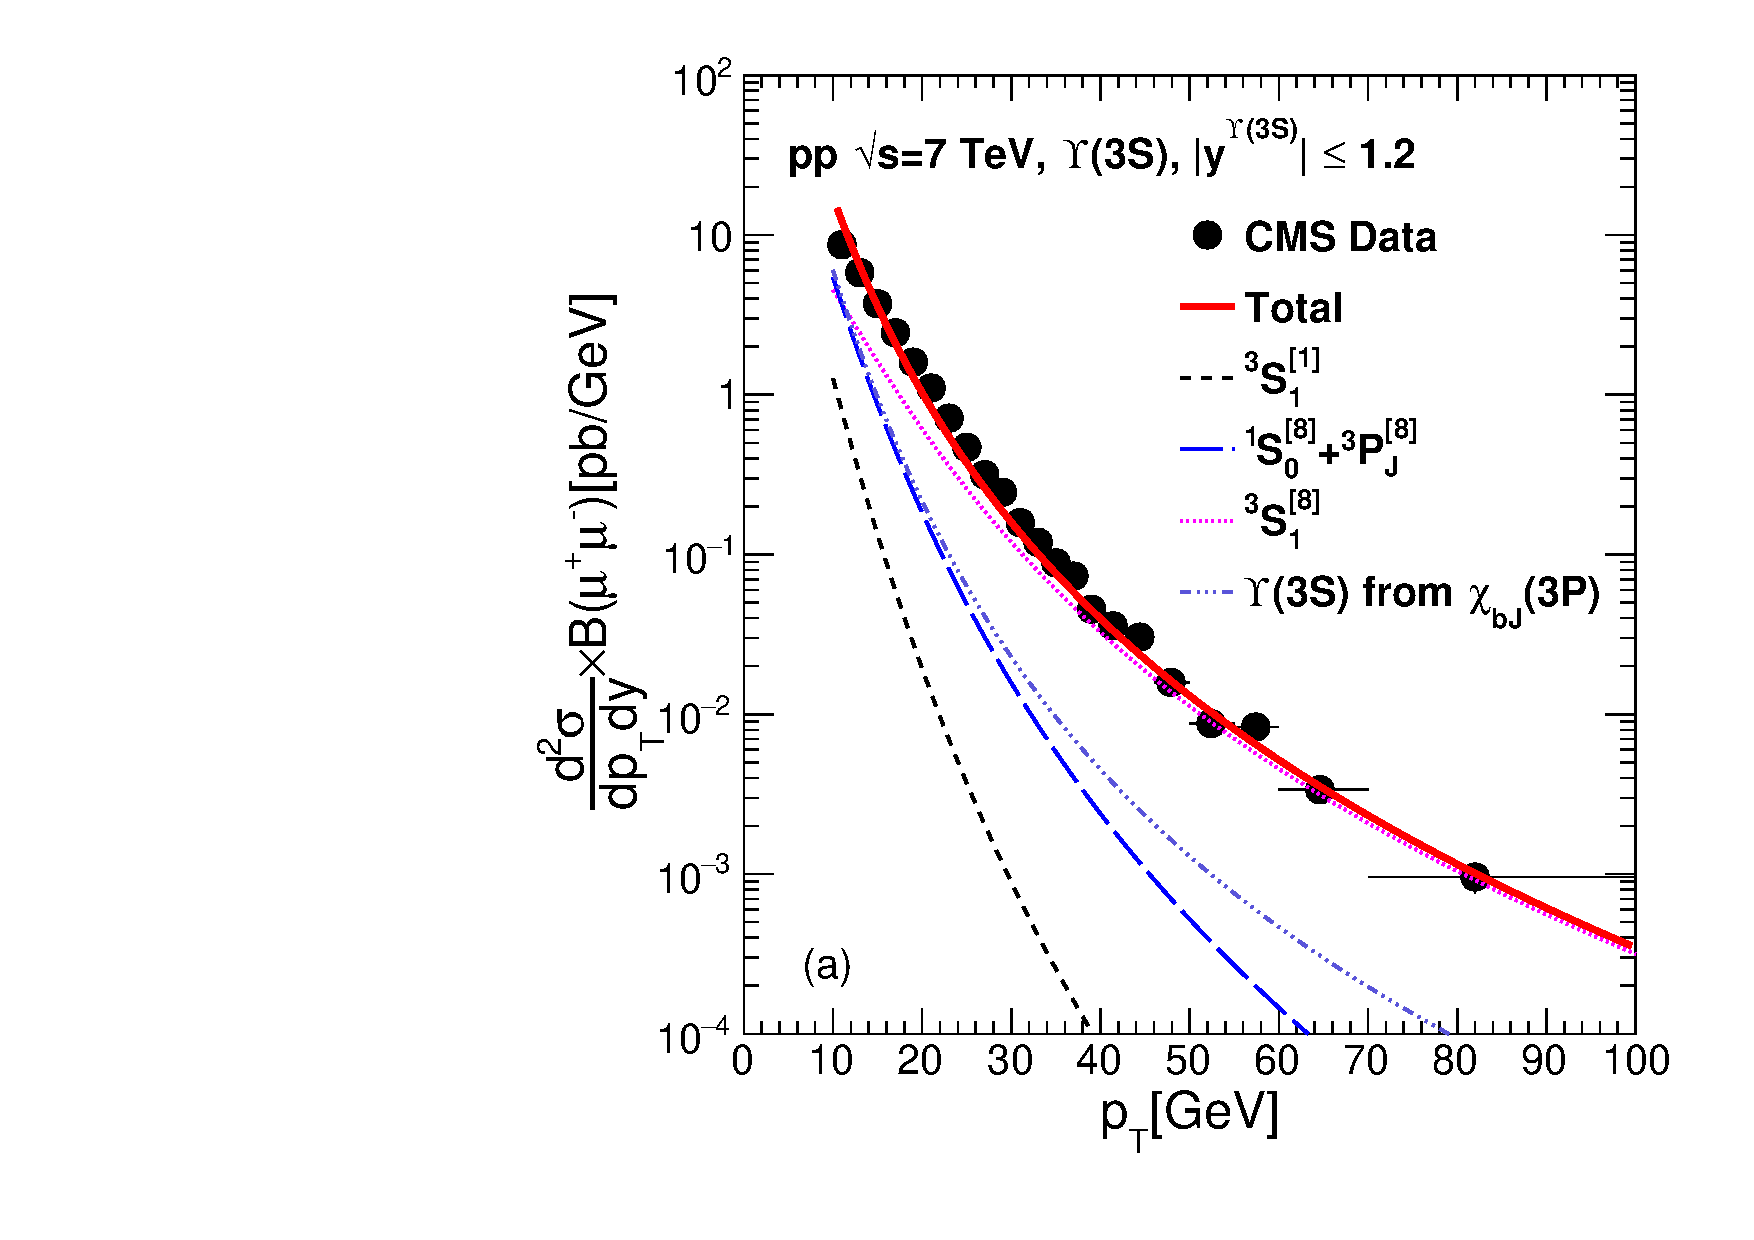
\includegraphics[width=0.49\textwidth]{Figures/NRQCD_Beauty/Fig1a_Y3S_CMS.pdf}
  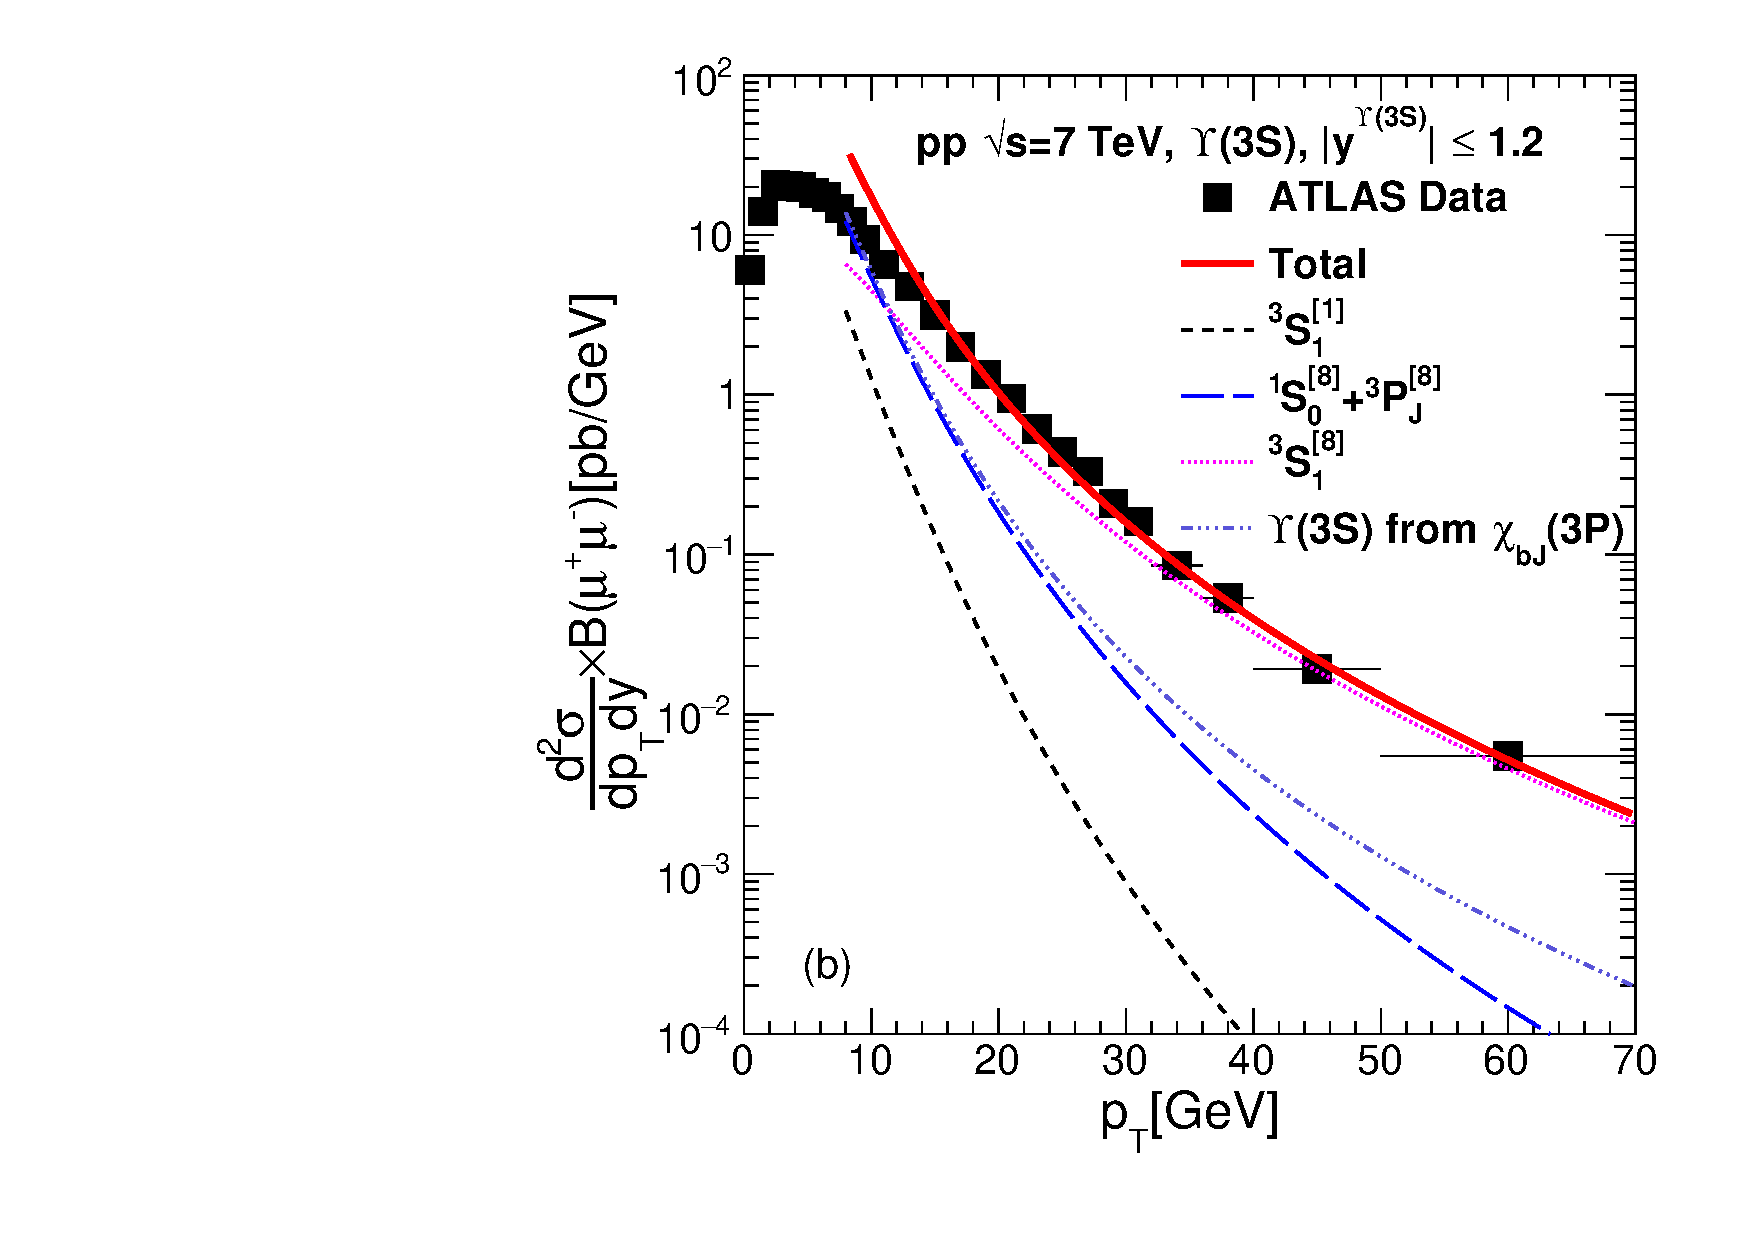
\includegraphics[width=0.49\textwidth]{Figures/NRQCD_Beauty/Fig1b_Y3S_ATLAS.pdf} 
  \caption{\small{The NRQCD calculations of production cross-section of $\Upsilon$(3S) in p+p collisions at 
      $\sqrt{s}$ = 7 TeV in central rapidities, as a function of transverse momentum compared with the measured data 
      at CMS~\cite{Khachatryan:2015qpa} and ATLAS~\cite{Aad:2012dlq} experiment.} }
  %   The LDMEs are obtained by a combined fit of the CMS and ATLAS data.}
  \label{Fig:SigmaY3SCMS}
\end{figure}

The contributions from CS-$[^3P_J]_1$ and CO-$[^3S_1]_8$ states are in the same order
of $v$ for the p-wave bound states, $\chi_{b}(nP)$. The angular momentum barriers of the p-wave
states are held responsible for that to happen and thereby making them important enough
to be considered. The differential cross-section for $\chi_b$ production
henceforth is given by,
\begin{eqnarray}
  d\sigma(\chi_{bJ}(1P)) &=& d\sigma(Q\overline{Q}([^3P_J]_{1}))
  M_{L}(Q\bar{Q}([^3P_J]_{1})\rightarrow \chi_{bJ}(1P)) \nonumber \\
  &+& d\sigma(Q\overline{Q}[^3S_1]_{8}))
  M_{L}(Q\bar{Q}([^3S_1]_{8})\rightarrow \chi_{bJ}(1P))  \nonumber \\
  &+& ...
  \label{eq9}
\end{eqnarray}

The experimental observations of $\Upsilon$ production at LHC energies, not only have contributions from
direct yield, but also consist of feed downs from decay of heavier bottomonia states.
The corresponding branching fractions are
provided in Table~\ref{BRUpsilon}.
%It is assumed that there is no significant feed down effect in $\Upsilon$(3S) from
%higher mass states like $\chi_{bJ}$(3P).

\begin{figure}[!h]
  \centering
  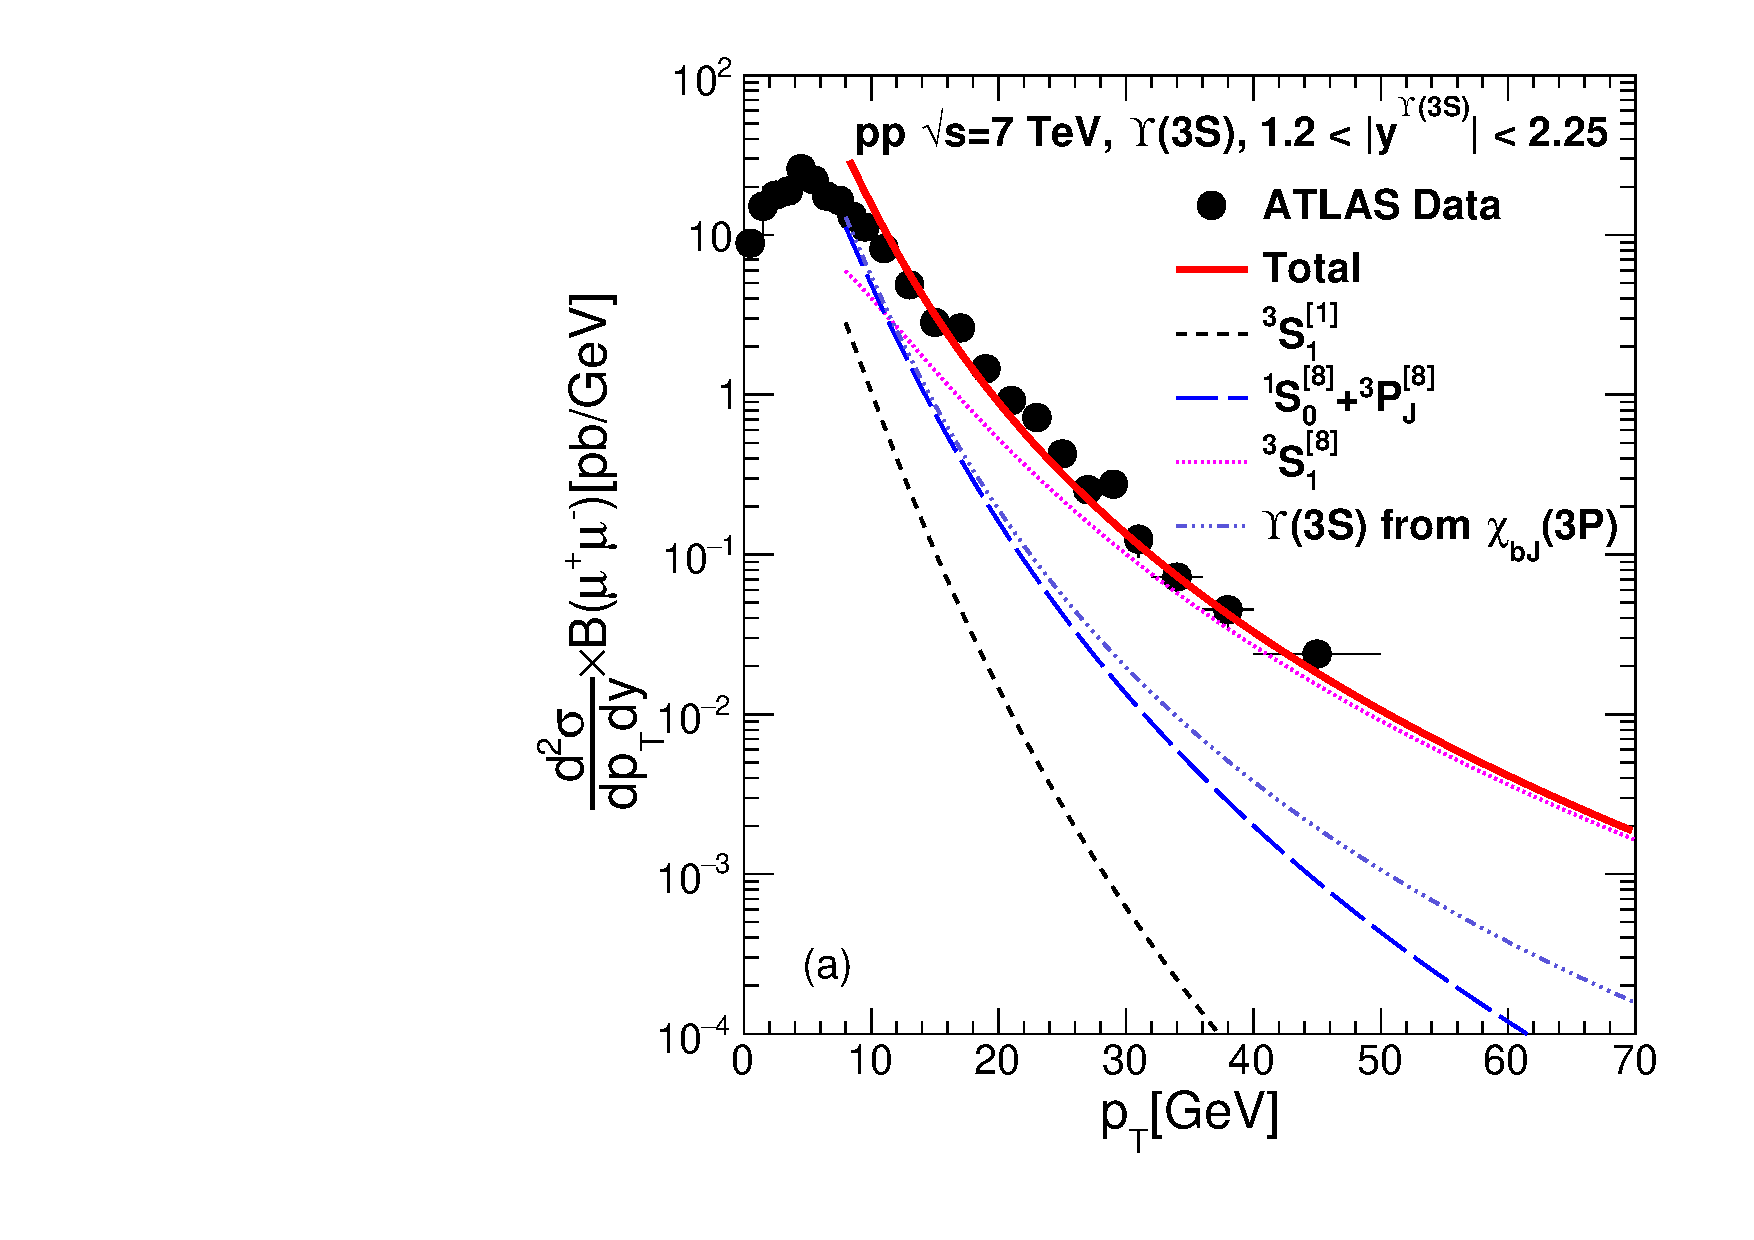
\includegraphics[width=0.49\textwidth]{Figures/NRQCD_Beauty/Fig2a_Y3S_ATLAS_Rap12225.pdf}
  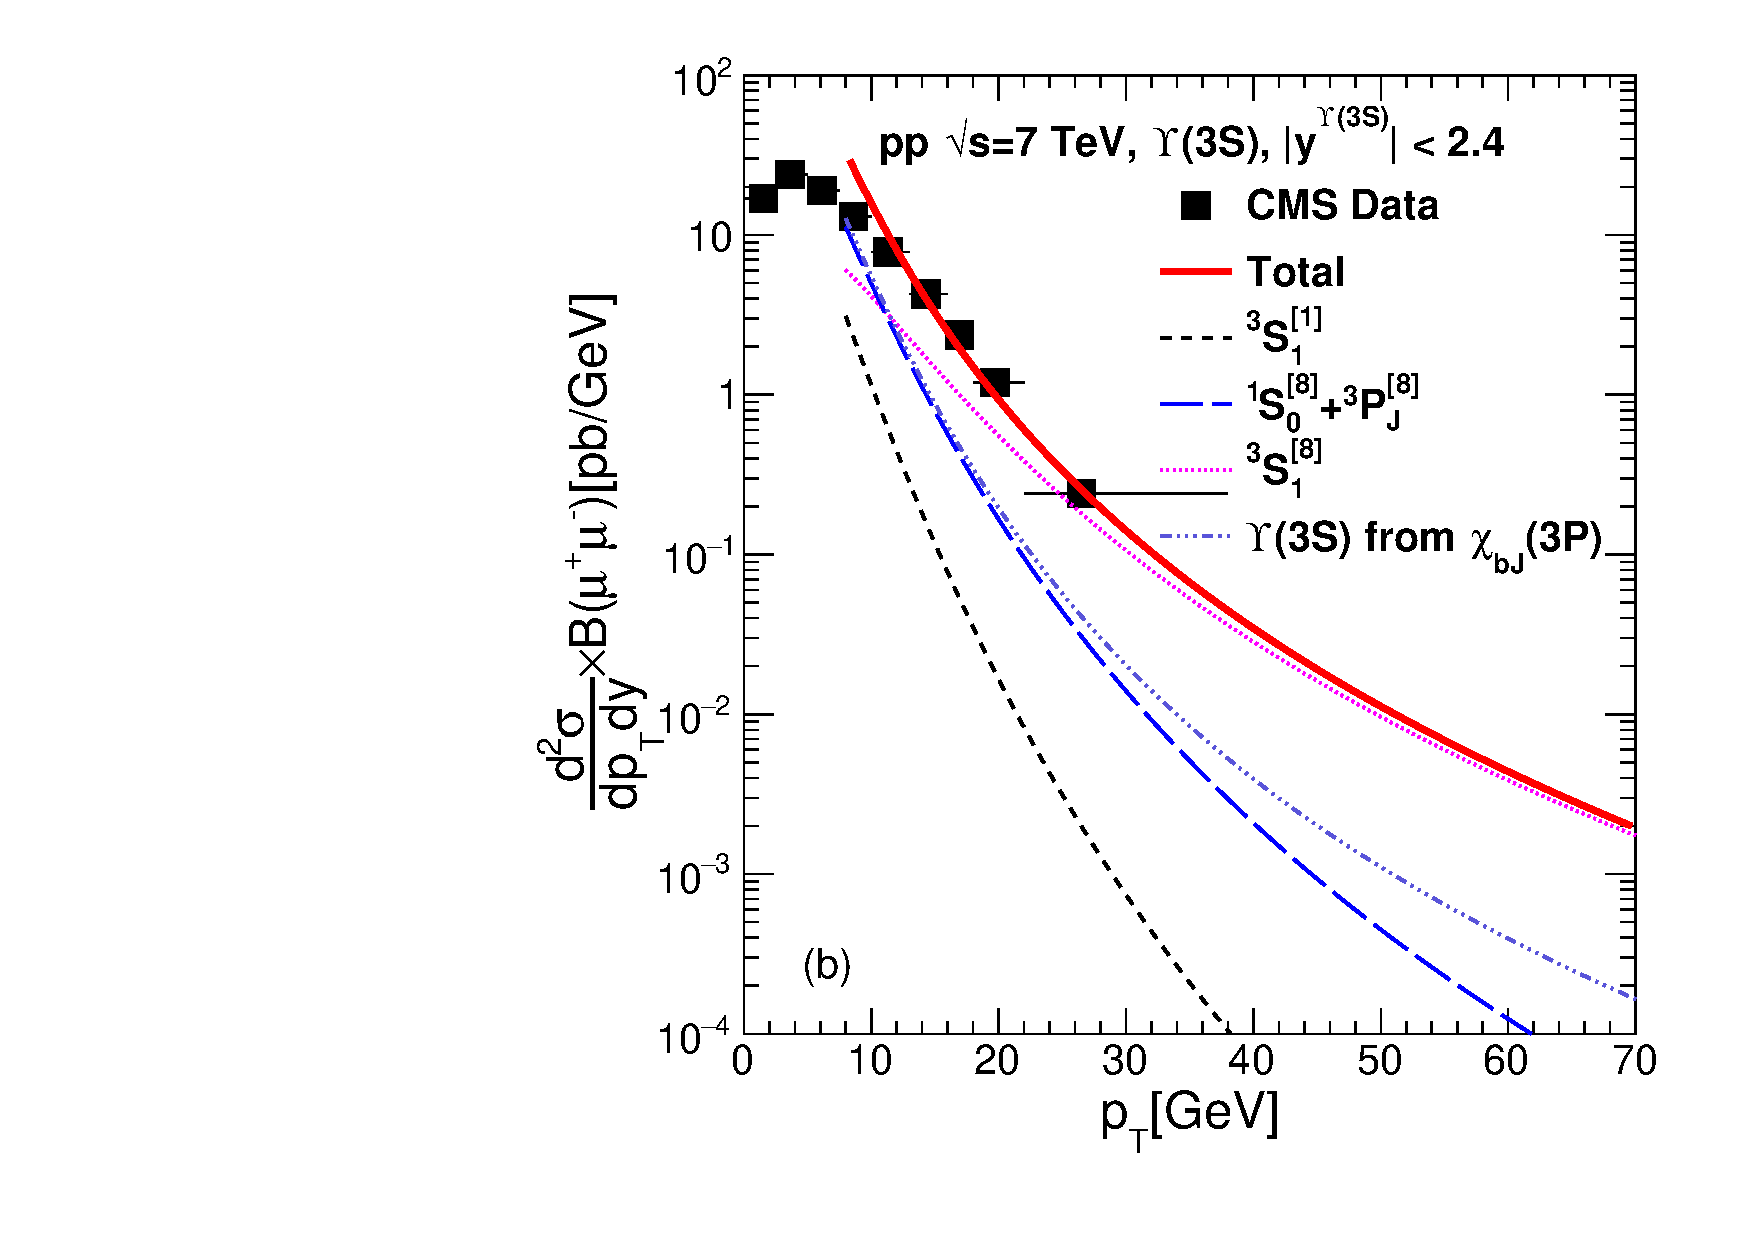
\includegraphics[width=0.49\textwidth]{Figures/NRQCD_Beauty/Fig2b_Y3S_CMS_Rapl24.pdf} 
  \caption{\small{The NRQCD calculations of production cross-section of $\Upsilon$(3S) in p+p collisions at 
      $\sqrt{s}$ = 7 TeV in forward rapidities, as a function of transverse momentum compared with the measured data 
      at ATLAS~\cite{Aad:2012dlq} and CMS~\cite{Chatrchyan:2013yna} experiments. }}
  %   The LDMEs are obtained by a combined fit of the CMS and ATLAS data.}
  \label{Fig:SigmaY3SCMS_forwardRap}
\end{figure}


We require both CS and CO matrix elements in order to get theoretical
predictions for the production of bottomonia at the Tevatron and LHC energies.
The corresponding expressions and
numerical values for CS states are obtained from Ref.~\cite{Brateen:PRD2001}.
The CO states, on the other hand, cannot be directly connected to the non-relativistic
wavefunctions of heavy mesons,
as these are associated with a higher Fock state. Experimentally measured data sets are 
therefore employed to obtain them as in Refs.~\cite{Brateen:PRD2001,Cho:1995vh,Cho:1995ce}. 
The CS operators along with their theoretical values
and the CO operators to be fitted are listed in Table~\ref{CSCO},
where, $n$=1,2,3. For the CO elements related to p-wave states, needed as the 
feed down contributions, we have used values obtained by Ref.~\cite{Sharma:2012dy,Feng:2015wka} for the 
present purpose. In our calculations, we have used
%CTEQ6L parametrisation \cite{Lai:2010vv} for parton distribution functions and
CT18NLO parametrisation~\cite{Hou:2019efy} for parton distribution functions and 
the bottom quark mass $m_b$ is taken to be 4.88 GeV.
The short distance cross-sections for $[^1S_0]_8$ and $[^3P_J]_8$ states having similar 
$p_T$ dependencies, the corresponding distributions become sensitive upto a linear combination
of their LDMEs. We therefore take resort to a linear combination following
Ref.~\cite{Kumar:2016ojy} as,

%\begin{align*}
\begin{equation*}
  \begin{split}
    & M_L(b\bar{b}([^1S_0]_8,[^3P_0]_8)\rightarrow\Upsilon(nS)) = \\
    &\frac{M_L(b\bar{b}([^1S_0]_8)\rightarrow\Upsilon(nS))}{5} +\frac{3 M_L(b\bar{b}([^3P_0]_8)\rightarrow\Upsilon(nS))}{m_b^2}.\\
  \end{split}
\end{equation*}
%\end{align*}
%\newpage
\begin{figure}
  \centering
  \includegraphics[width=0.49\textwidth]{Figures/NRQCD_Beauty/Fig3a_Y3S_CMS_13TeV_Rap06.pdf}
  \includegraphics[width=0.49\textwidth]{Figures/NRQCD_Beauty/Fig3b_Y3S_CMS_13TeV_Rap0612.pdf}
  \includegraphics[width=0.49\textwidth]{Figures/NRQCD_Beauty/Fig3c_Y3S_CMS_13TeV_Rap12.pdf}
  \caption{\small{The NRQCD calculations of production cross-section of $\Upsilon$(3S) in p+p collisions at 
      $\sqrt{s}$ = 13 TeV in central and forward rapidities, as a function of transverse momentum compared with the measured data 
      at CMS~\cite{Sirunyan:2017qdw} experiment. }}
  %   The LDMEs are obtained by a combined fit of the CMS and ATLAS data.}
  \label{Fig:SigmaY3SCMS13TeV}
\end{figure}

\begin{table*}
  \centering
  \caption{Comparison of CS elements and CO LDMEs extracted from fitting with experimental data
    using NRQCD formalism for $\Upsilon$(3S).}
  \footnotesize
  %\begin{tabular}{ccccccc}
  \begin{tabular*}{\textwidth}{@{\extracolsep{\fill}}lrrrrrl@{}}
    \hline
    \hline
    %& & & & & & \\
    Ref. (LO/NLO) &PDF & $m_b$ & $M_L(b\bar{b}([^3S_1]_1$ & $M_L(b\bar{b}([^3S_1]_8$ & 
    $M_L(b\bar{b}([^1S_0]_8$, & $p_T$-cut \\
    & & & $\rightarrow\Upsilon(3S)$ & $\rightarrow\Upsilon(3S)$ & $[^3P_0]_8\rightarrow\Upsilon(3S)$ & \\
    & & (GeV) & $({\rm GeV^3})$ & $({\rm GeV^3})$ & $({\rm GeV^3})$ & GeV/$c$ \\
    %& & & & & & \\
    \hline
    \hline
    & & & & & & \\
    present (LO) & CT18 &4.88 &4.3 & 0.0543$\pm$0.0007 & 0.0097$\pm$0.0005 & 8   \\
    % & (LO) & & & & & \\
    %\hline
    & & & & & & \\
    \cite{Domenech:2000ri} (LO) & CTEQ4L & 4.88 & 3.54 & 0.099$\pm$0.011 & 0 & 2 \\
    & & & & 0.091$\pm$0.015 & 0 & 4 \\
    & & & & 0.068$\pm$0.011 & 0 & 8 \\
    & & & & & & \\
    %\hline
    %& & & & & & \\
    \cite{Brateen:PRD2001} (LO) & CTEQ5L & 4.77 & 4.3$\pm$0.9 & 0.036$\pm$0.019 & 0.0108$\pm$0.0086 & 8 \\
    & & & & 0.039$\pm$0.017 & 0.0342$\pm$0.0276 & \\
    & & & & & & \\
    & MRSTLO & 4.77 & 4.3$\pm$0.9 & 0.037$\pm$0.021 & 0.0150$\pm$0.0098 & 8 \\
    & & & & 0.041$\pm$0.019 & 0.0474$\pm$0.0312 & \\
    & & & & & & \\
    %\hline
    %& & & & & & \\
    \cite{Gong:2010bk} (NLO) & CTEQ6M & 5.18 & 1.128 & 0.03250$\pm$0.00876 & 0.000920$\pm$0.000968 & -\\
    %& (NLO) & & & & & \\
    %\hline
    & & & & & & \\
    \cite{Sharma:2012dy} (LO) & MSTW08LO & 4.88 & 4.3 & 0.0513$\pm$0.0085 & 0.0002$\pm$0.0062 & -  \\
    %& (LO) & & & & & \\
    %\hline
    & & & & & & \\
    \cite{Gong:2013qka} (NLO) & CTEQ6M & 5.18 & 1.128 & 0.0271$\pm$0.0013 & 0.00956$\pm$0.00476 & 8 \\
    %& (NLO) & & & & & \\
    %\hline
    & & & & & & \\
    \cite{Feng:2015wka} (NLO) & CTEQ6M & 5.18 & 1.128 & 0.0132$\pm$0.0020 & -0.00520$\pm$0.00518 & 8 \\
    %& (NLO) & & & & & \\
    \hline
    \hline
  \end{tabular*}
  \label{LDMEsY3S}
\end{table*}
\normalsize
%\newpage
%\subsection*{$\Upsilon$(2S)}

\begin{figure}
  \centering
  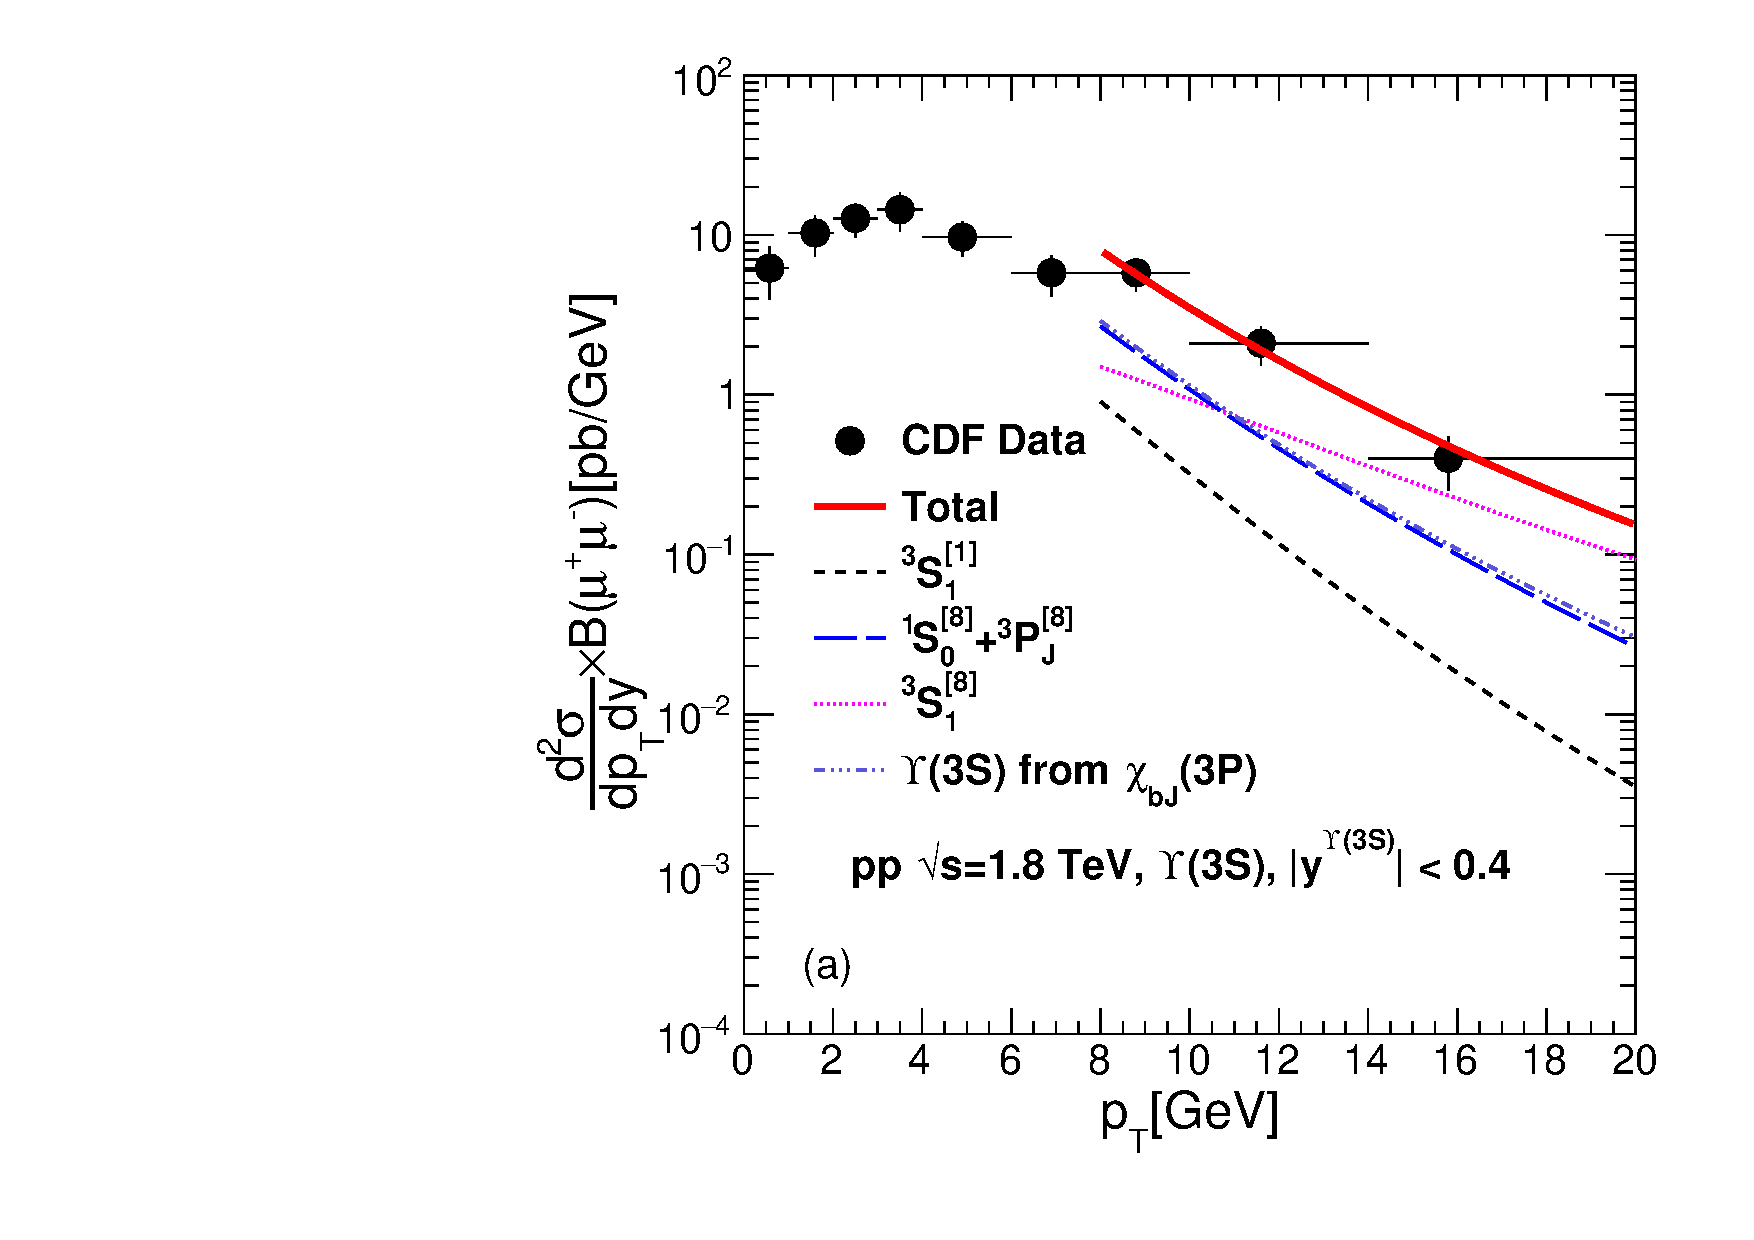
\includegraphics[width=0.49\textwidth]{Figures/NRQCD_Beauty/Fig4a_Y3S_CDF_180GeV_Rap2025.pdf}
  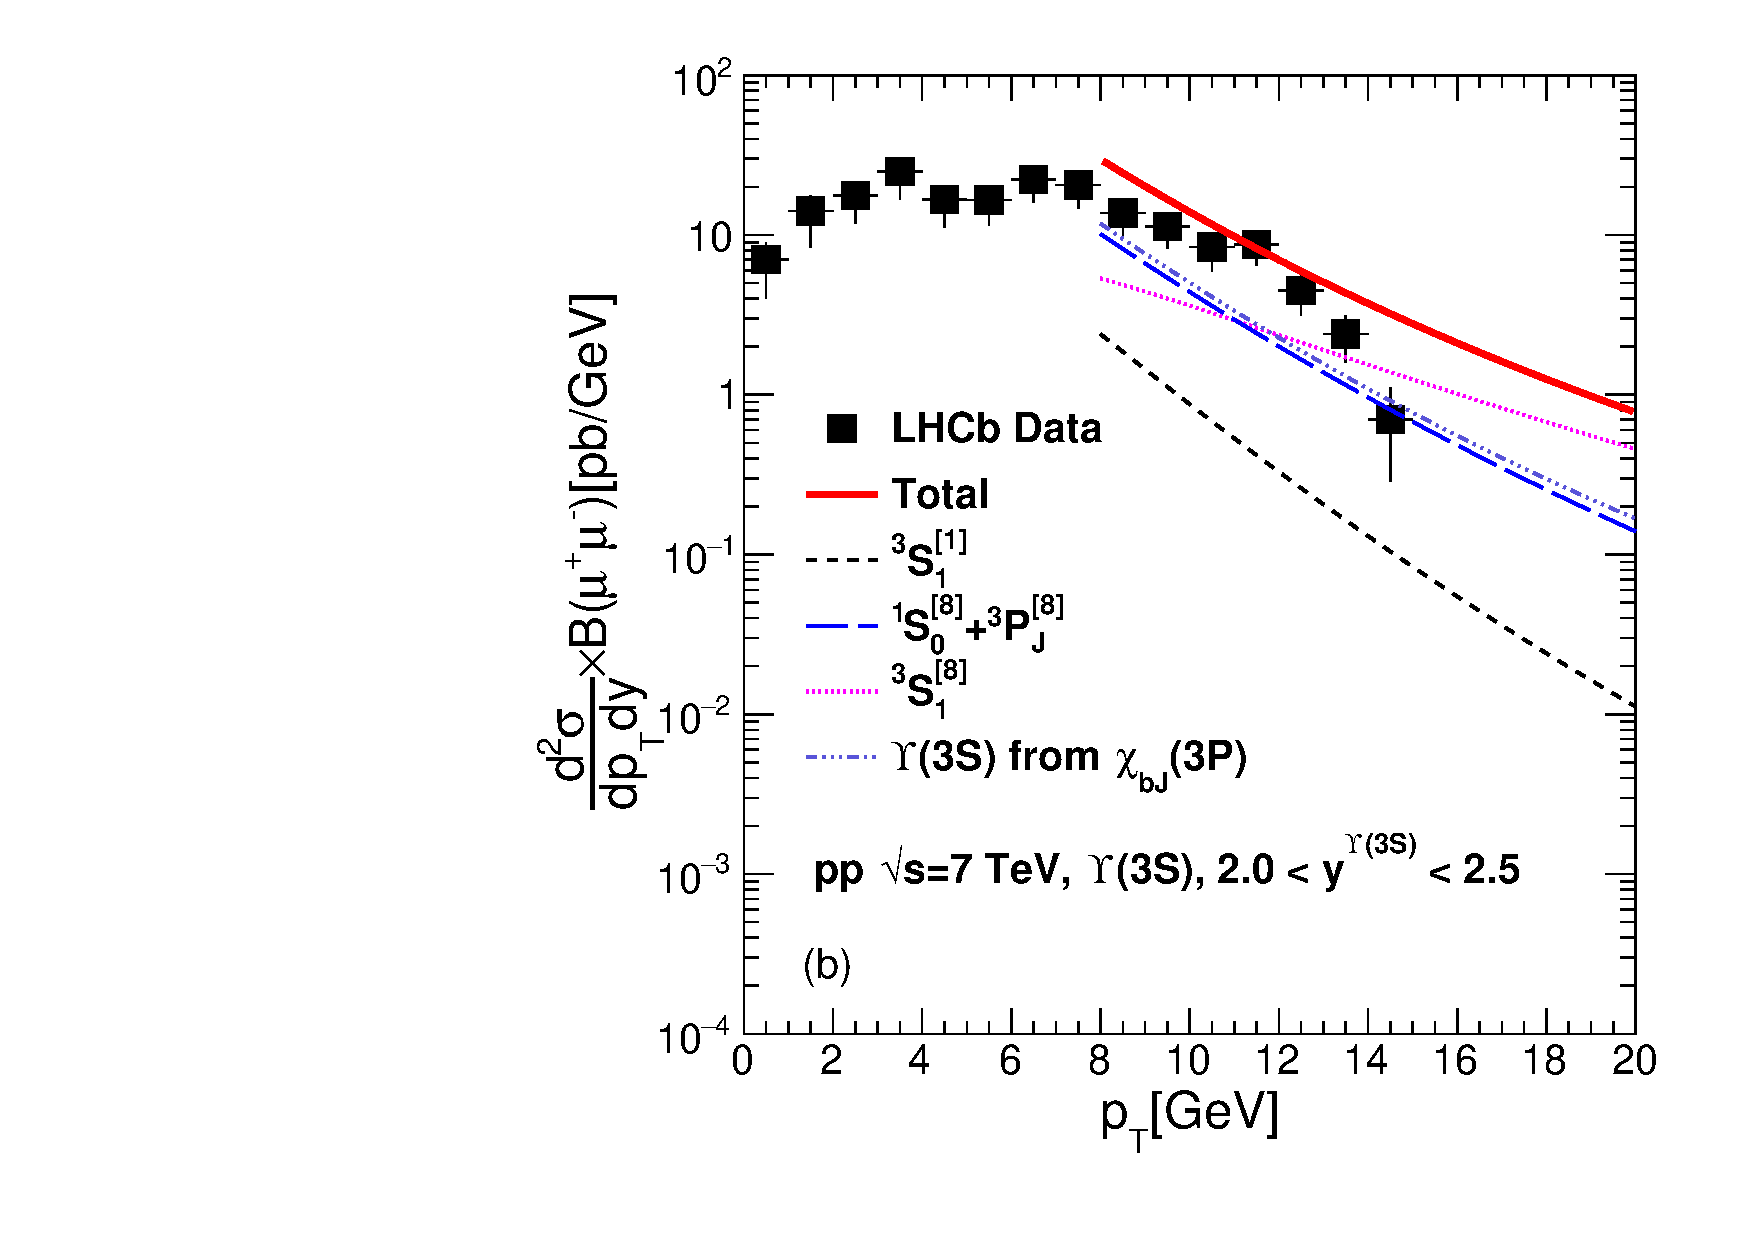
\includegraphics[width=0.49\textwidth]{Figures/NRQCD_Beauty/Fig4b_Y3S_LHCb_7TeV_Rap2025.pdf} 
  \caption{\small{The NRQCD calculations of production cross-section of $\Upsilon$(3S) in
      p +{$\bar {\rm p}$} collisions at $\sqrt{s}$ = 1.8 TeV and p+p collisions at
      7 TeV in forward rapidities, as a function of transverse momentum compared with the measured data 
      at CDF~\cite{Acosta:2001gv} and LHCb~\cite{LHCb:2012aa} experiment. }}
  %   The LDMEs are obtained by a combined fit of the CMS and ATLAS data.}
  \label{Fig:SigmaY3SCDF}
\end{figure}




%\begin{figure}
%\begin{minipage}{1.0\linewidth}
%\centering
%  {\includegraphics[width=0.42\textwidth]{Fig3a_Y3S_CMS_13TeV_Rap06.pdf}}
%  {\includegraphics[width=0.42\textwidth]{Fig3b_Y3S_CMS_13TeV_Rap0612.pdf}}
%\end{minipage}
%\ \\
%\centering
%\begin{minipage}{0.5\linewidth}
%\centering
%  {\includegraphics[width=0.84\textwidth]{Fig3c_Y3S_CMS_13TeV_Rap12.pdf}}
%  \end{minipage}
% \caption{The NRQCD calculations of production cross-section of $\Upsilon$(3S) in p+p collisions at 
%   $\sqrt{s}$ = 13 TeV in central and forward rapidities, as a function of transverse momentum compared with the measured data 
%   at CMS~\cite{Sirunyan:2017qdw} experiment. }
%%%   The LDMEs are obtained by a combined fit of the CMS and ATLAS data.}
%  \label{Fig:SigmaY3SCMS13TeV}
%\end{figure}

\begin{figure}
  \centering
  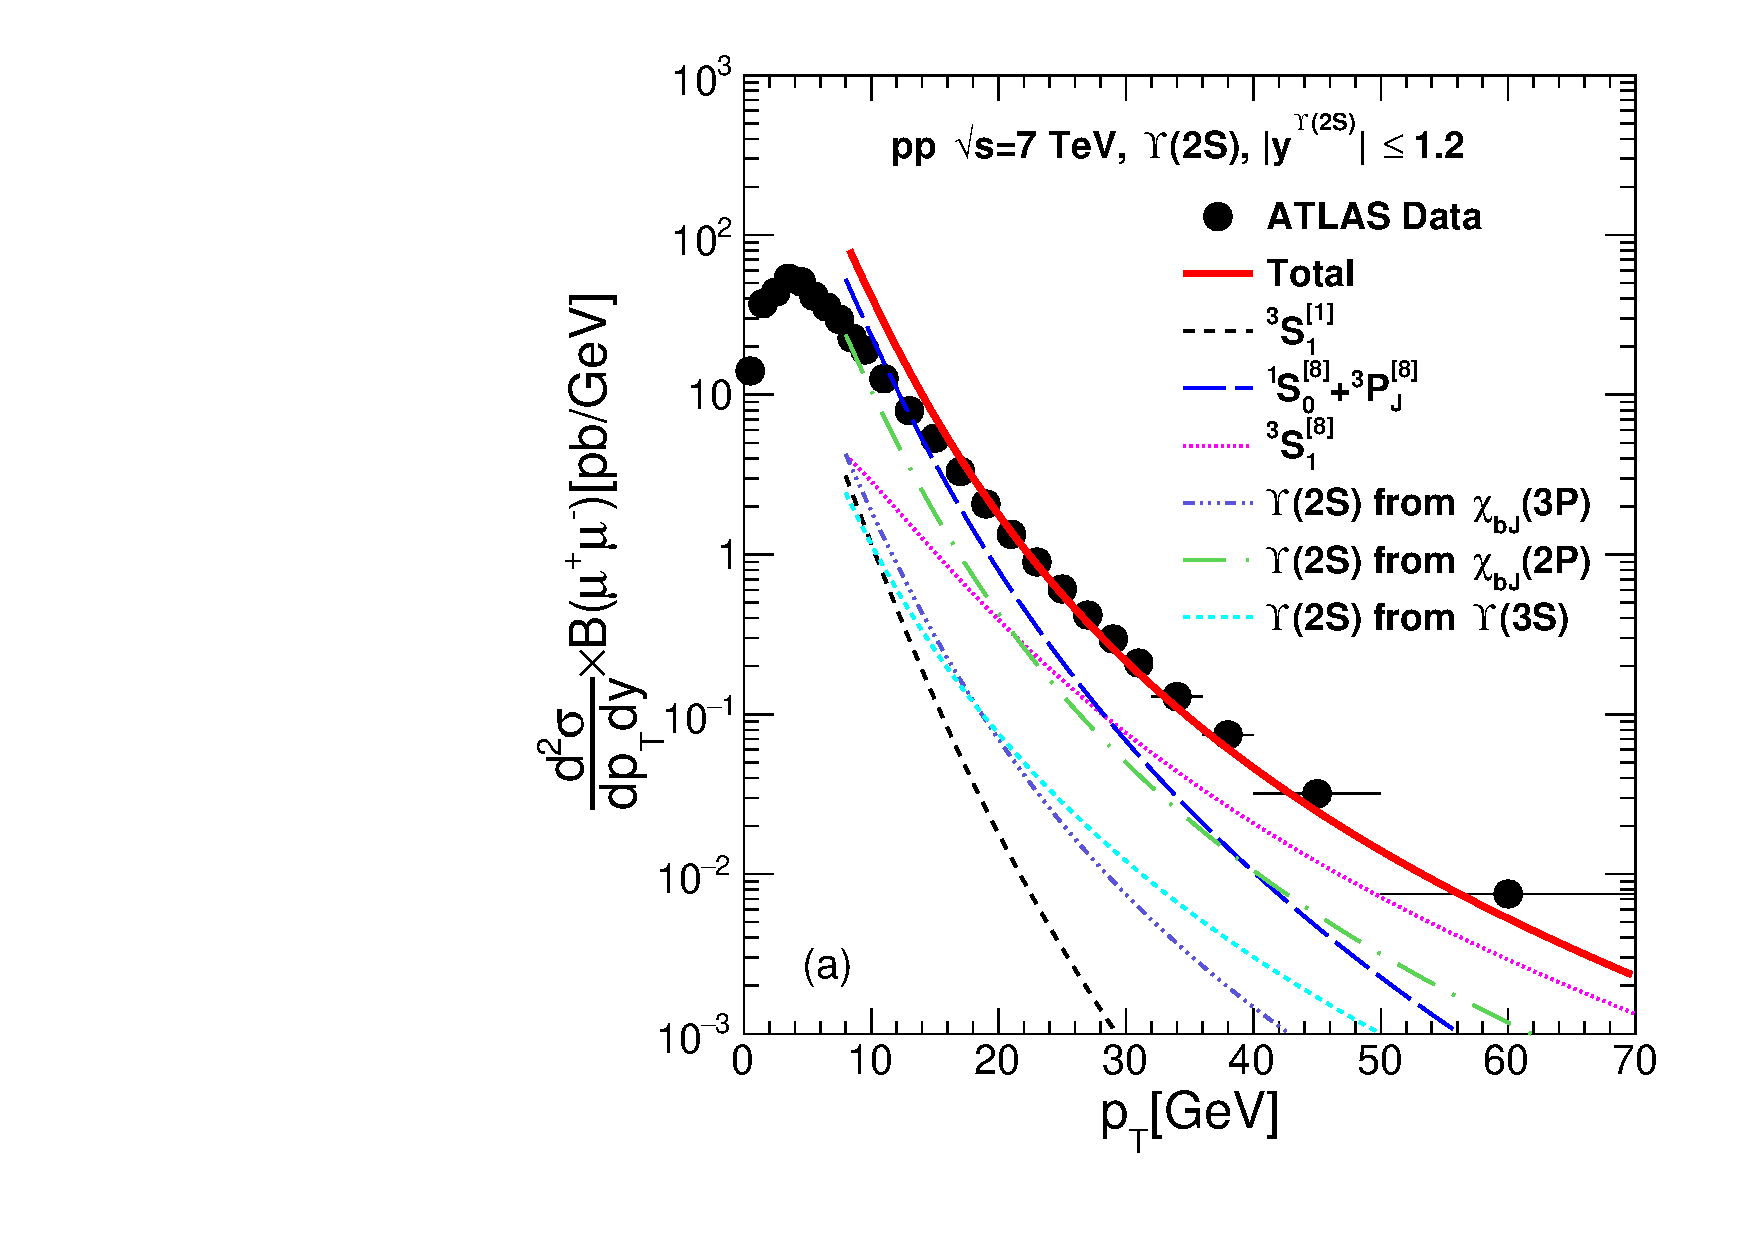
\includegraphics[width=0.49\textwidth]{Figures/NRQCD_Beauty/Fig5a_ATLAS_D2NDPtDy_Y2S_Y1212_Pt.pdf}
  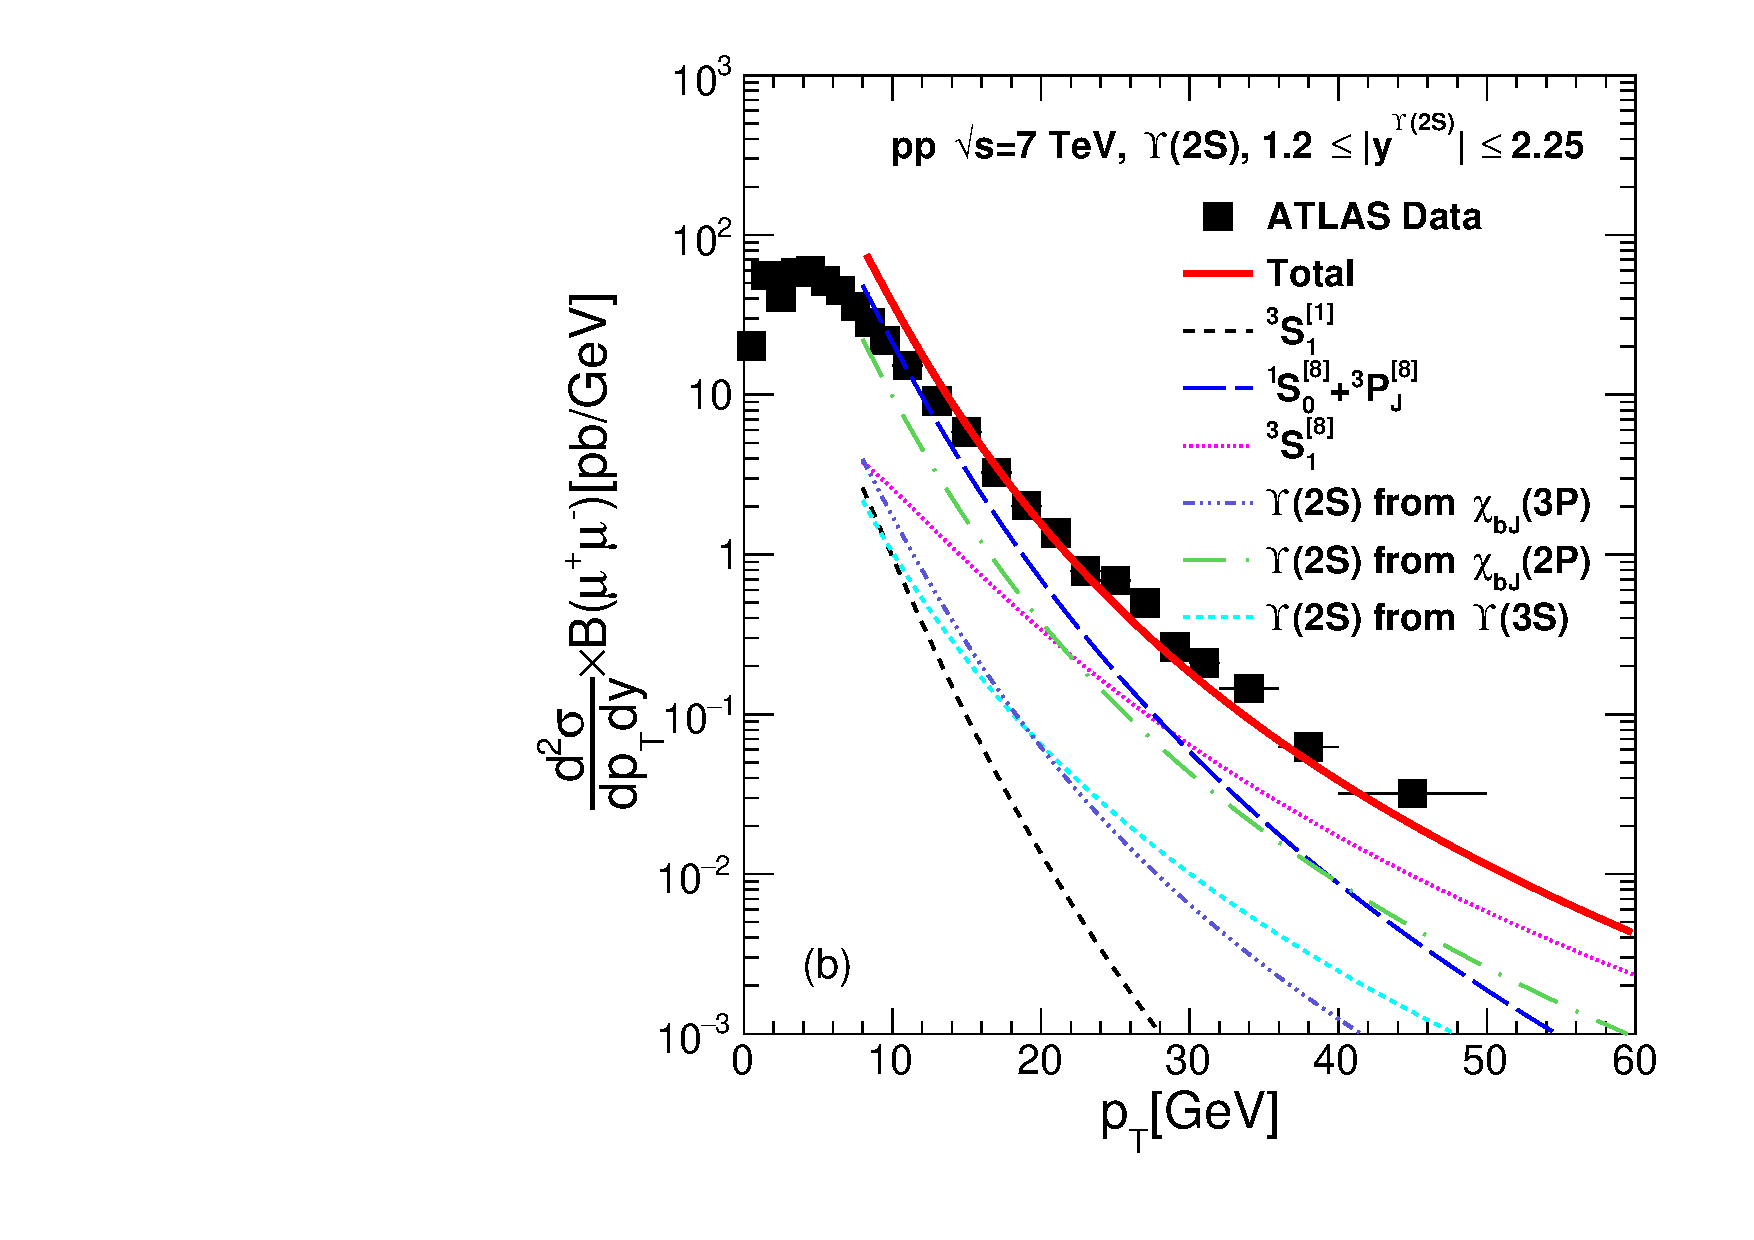
\includegraphics[width=0.49\textwidth]{Figures/NRQCD_Beauty/Fig5b_ATLAS_D2NDPtDy_Y2S_Y12225_Pt.pdf}
  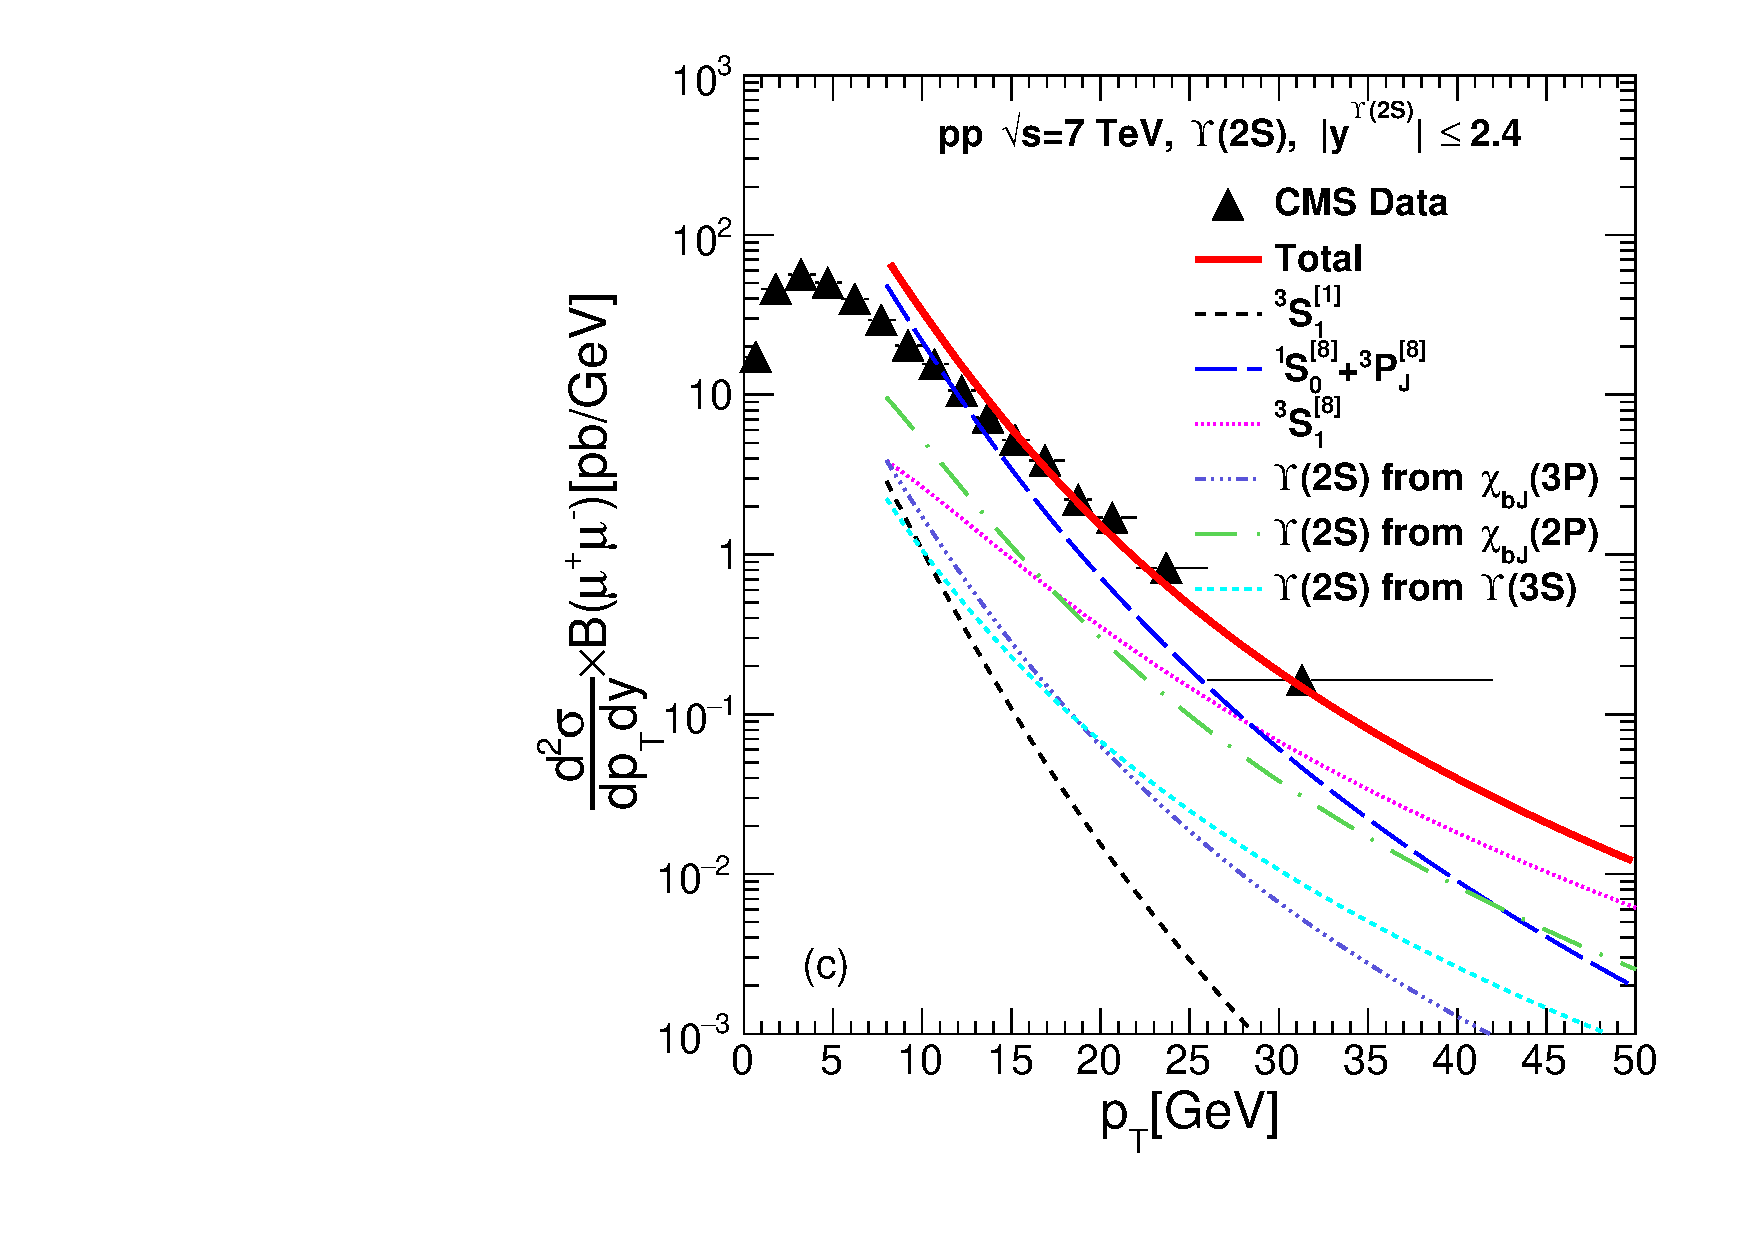
\includegraphics[width=0.49\textwidth]{Figures/NRQCD_Beauty/Fig5c_CMS_D2NDPtDy_Y2S_Y0024_Pt.pdf}
  \caption{\small{The NRQCD calculations of production cross-section of $\Upsilon$(2S) in p+p collisions at 
      $\sqrt{s}$ = 7 TeV in central and forward rapidities, as a function of transverse momentum compared with the measured data 
      at CMS~\cite{Chatrchyan:2013yna} and ATLAS~\cite{Aad:2012dlq} experiments. }}
  \label{Fig:SigmaY2SATLAS}
\end{figure}

\begin{figure}
  \centering
  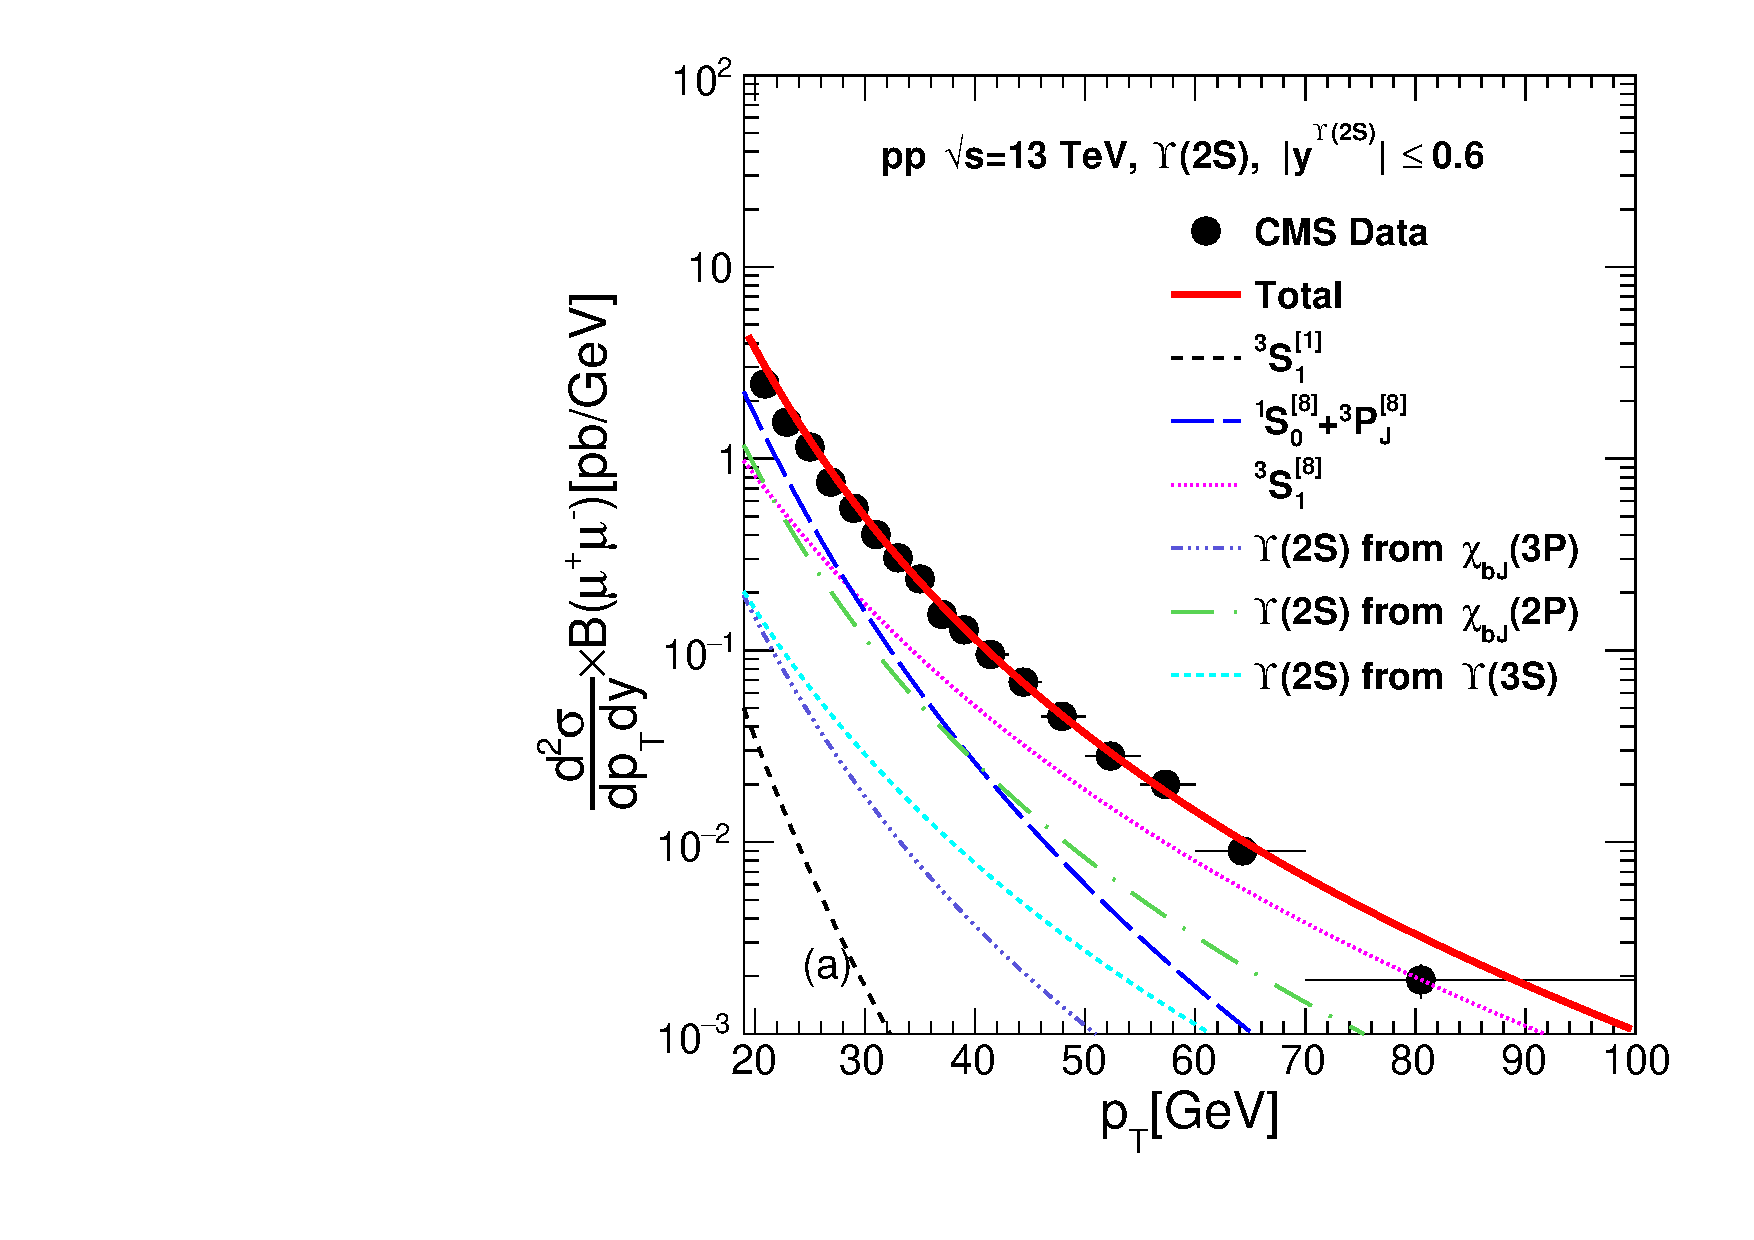
\includegraphics[width=0.49\textwidth]{Figures/NRQCD_Beauty/Fig6a_CMS_D2NDPtDy_Y2S_13TeV_Y0006_Pt.pdf}
  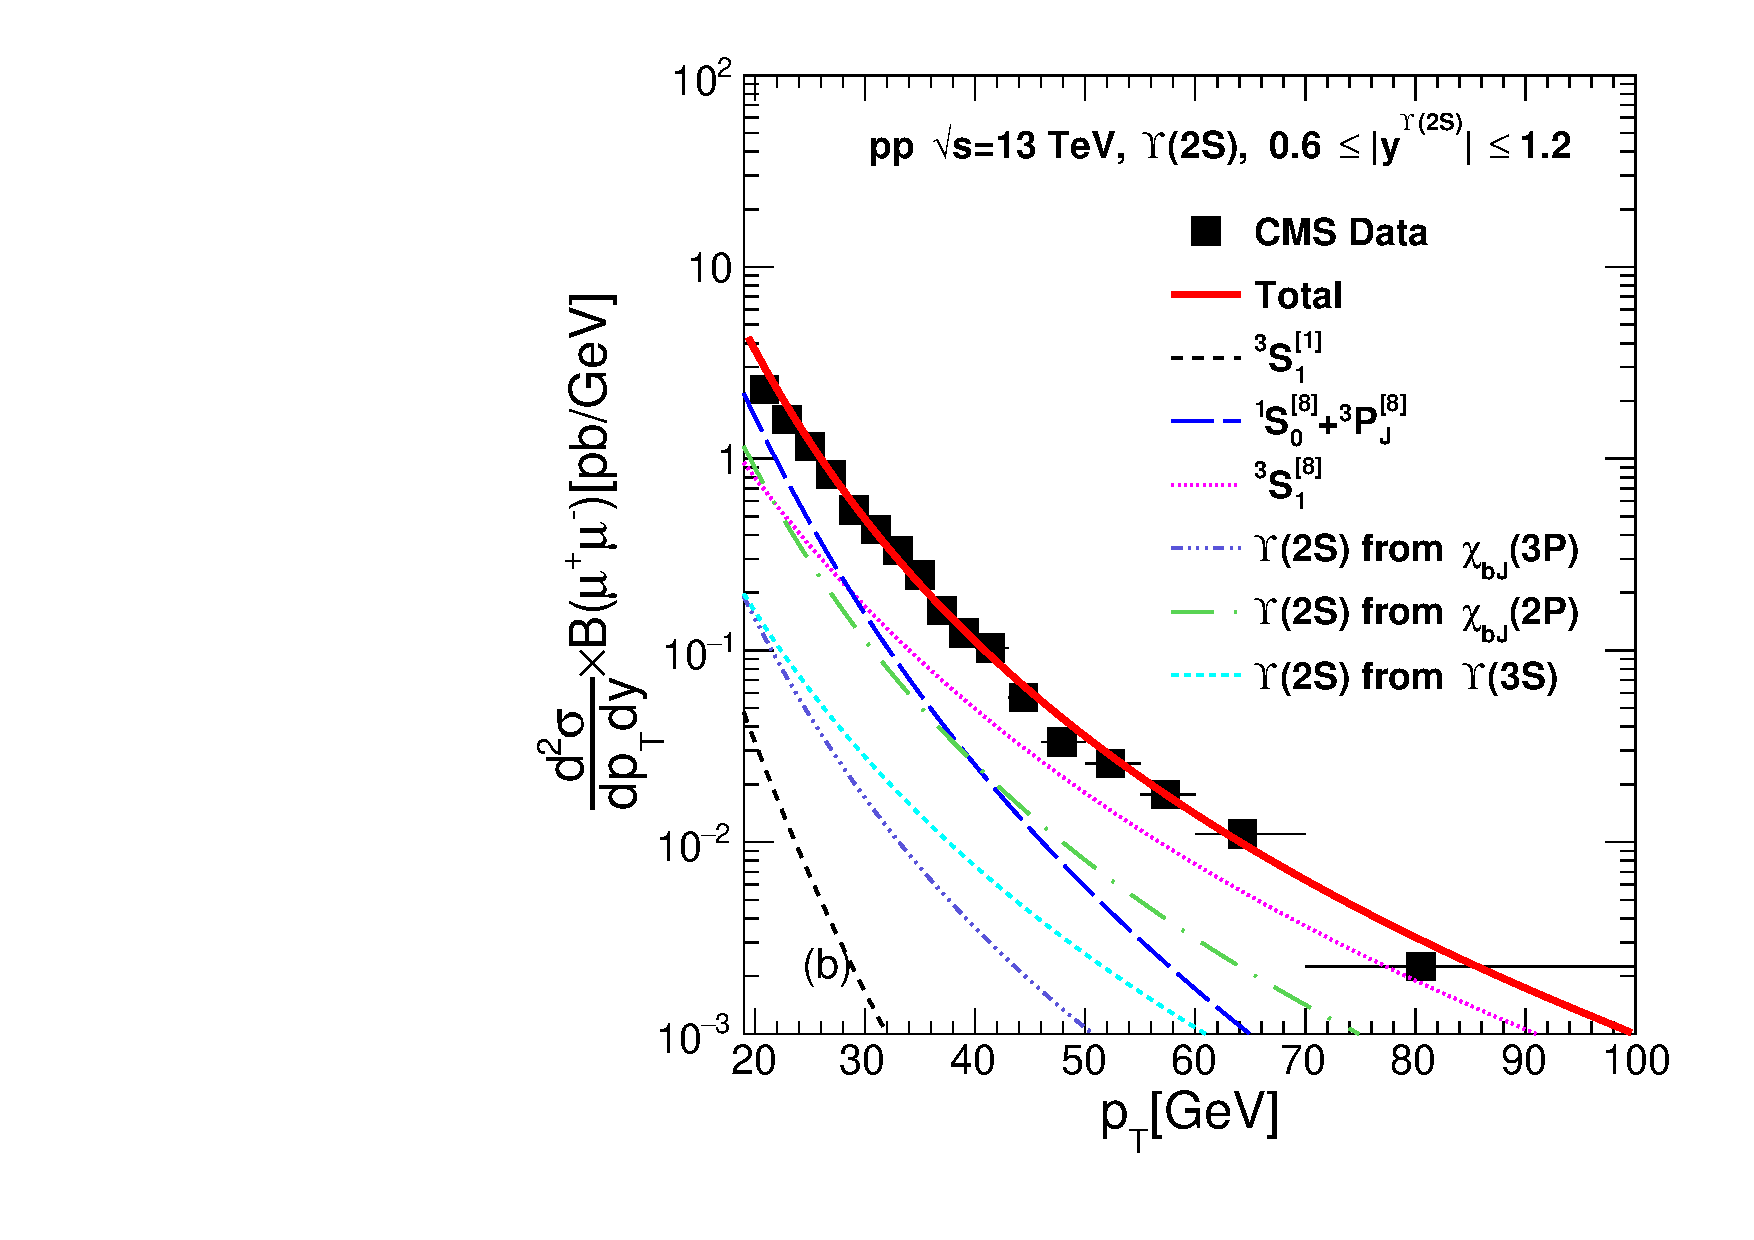
\includegraphics[width=0.49\textwidth]{Figures/NRQCD_Beauty/Fig6b_CMS_D2NDPtDy_Y2S_13TeV_Y0612_Pt.pdf} 
  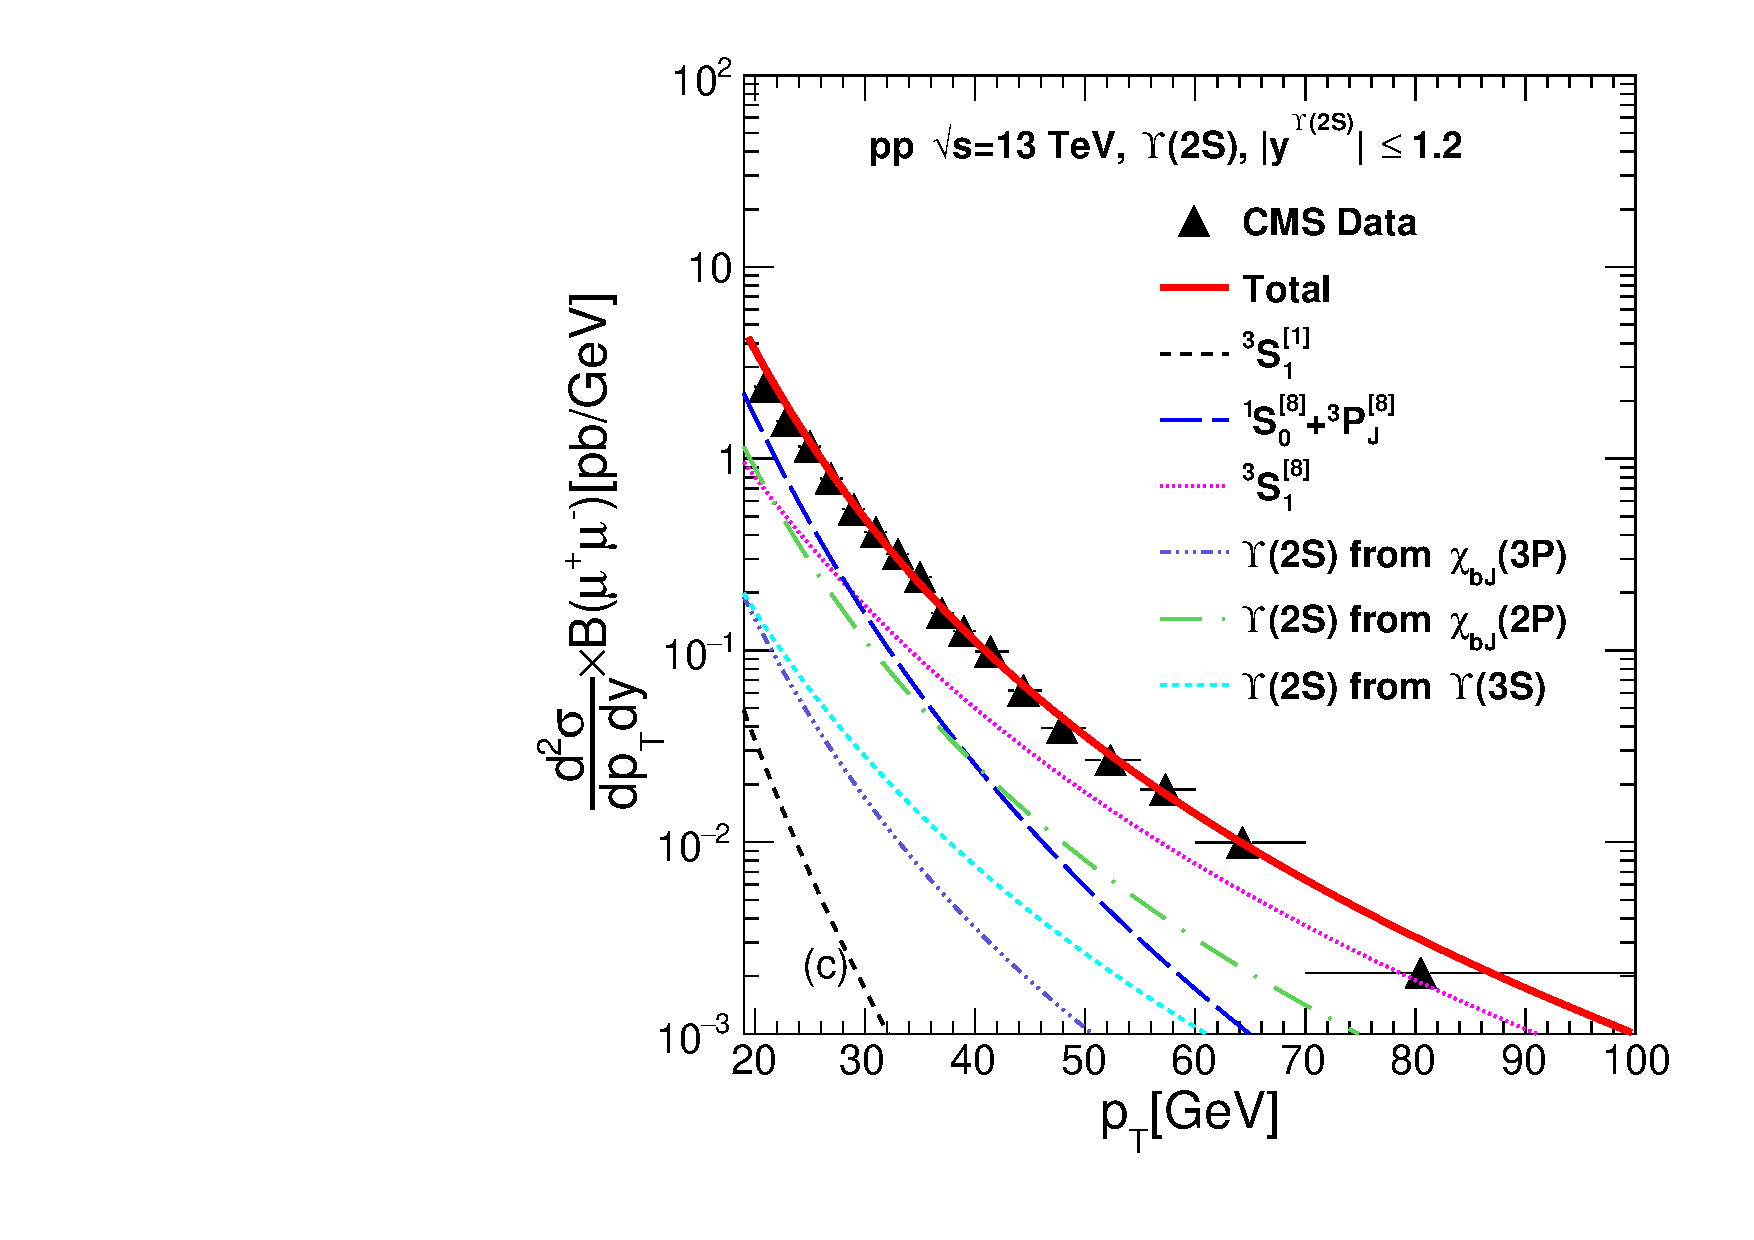
\includegraphics[width=0.49\textwidth]{Figures/NRQCD_Beauty/Fig6c_CMS_D2NDPtDy_Y2S_13TeV_Y0012_Pt.pdf}
  \caption{\small{The NRQCD calculations of production cross-section of $\Upsilon$(2S) in p+p collisions at 
      $\sqrt{s}$ = 13 TeV in central and forward rapidities, as a function of transverse momentum compared with the measured data 
      at CMS~\cite{Sirunyan:2017qdw} experiment. }}
  %   The LDMEs are obtained by a combined fit of the CMS and ATLAS data.}
  \label{Fig:SigmaY2SCMS13TeV}
\end{figure}

\begin{figure}
  \centering
  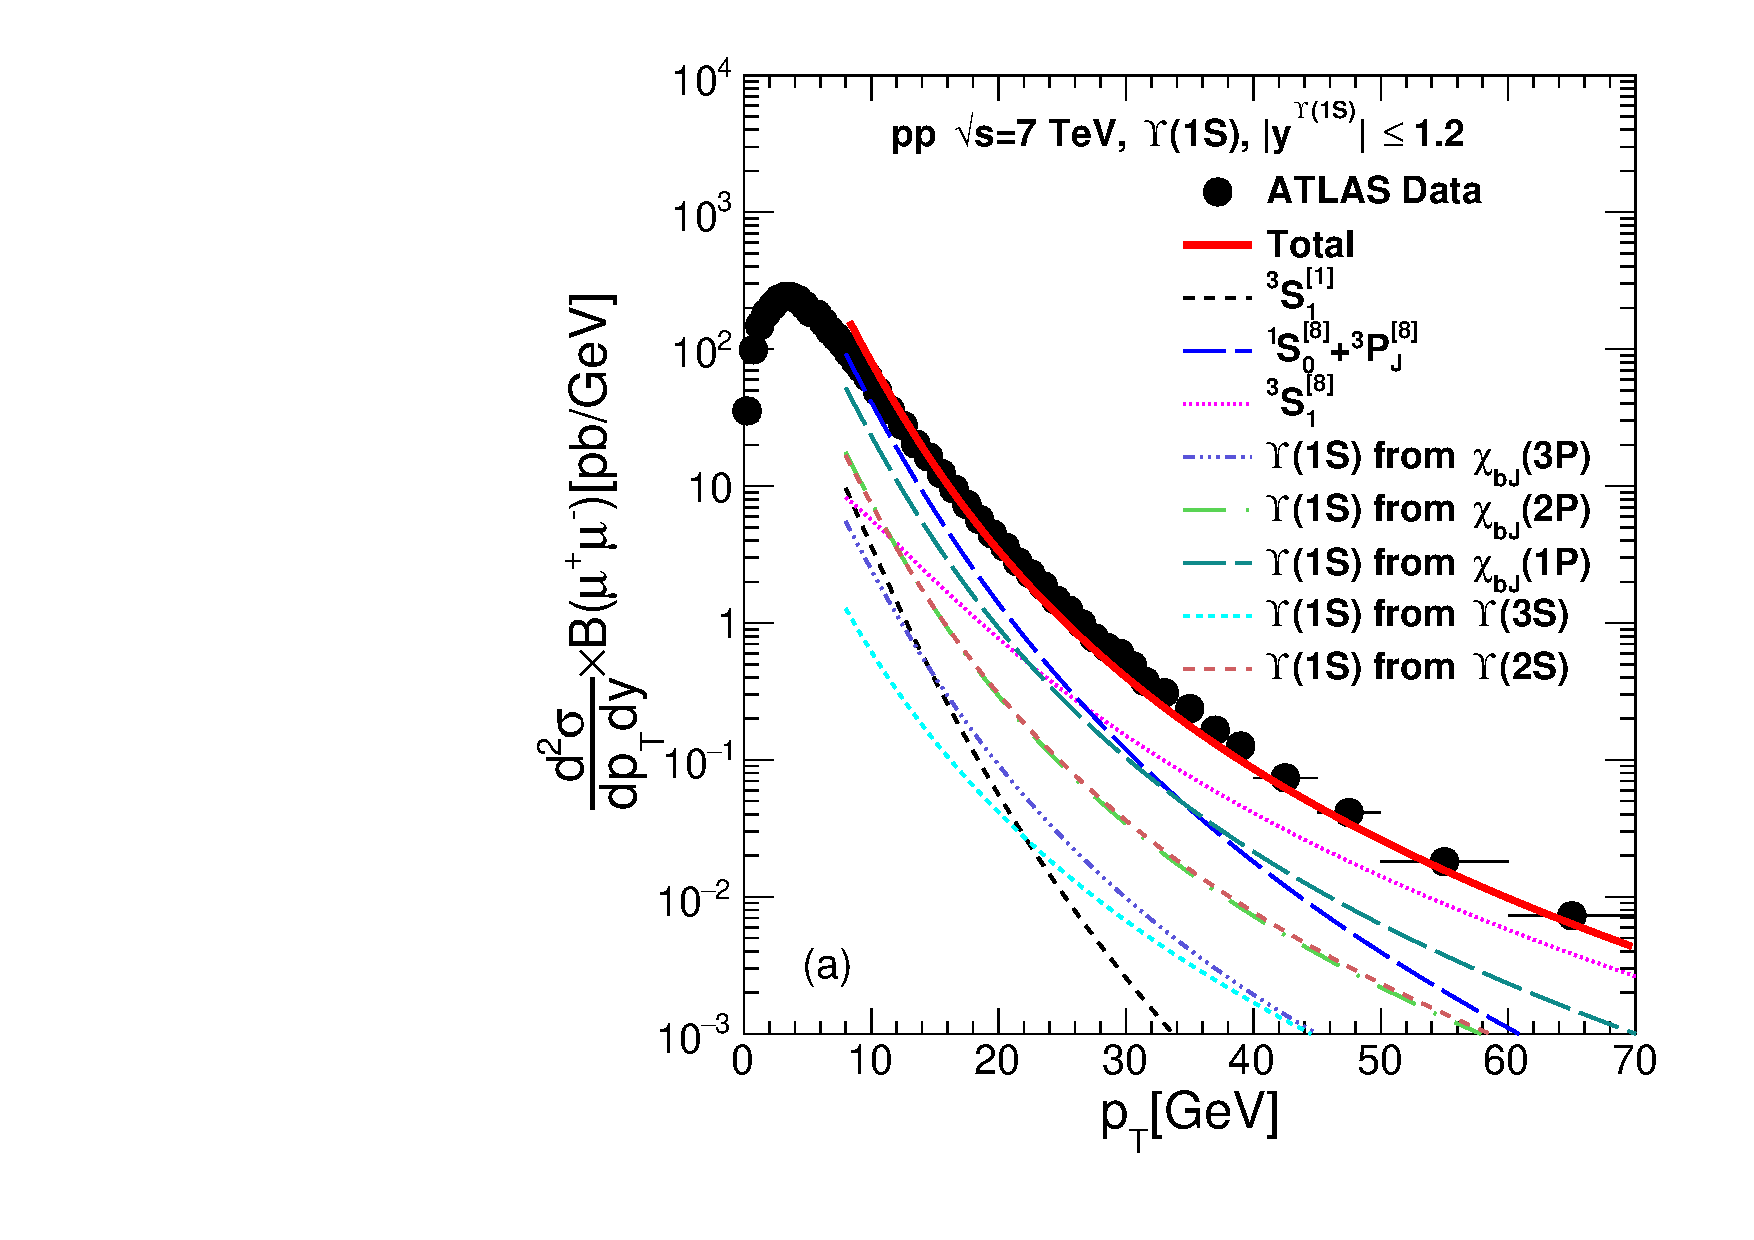
\includegraphics[width=0.49\textwidth]{Figures/NRQCD_Beauty/Fig7a_ATLAS_D2NDPtDy_Y1S_Y1212_Pt.pdf}
  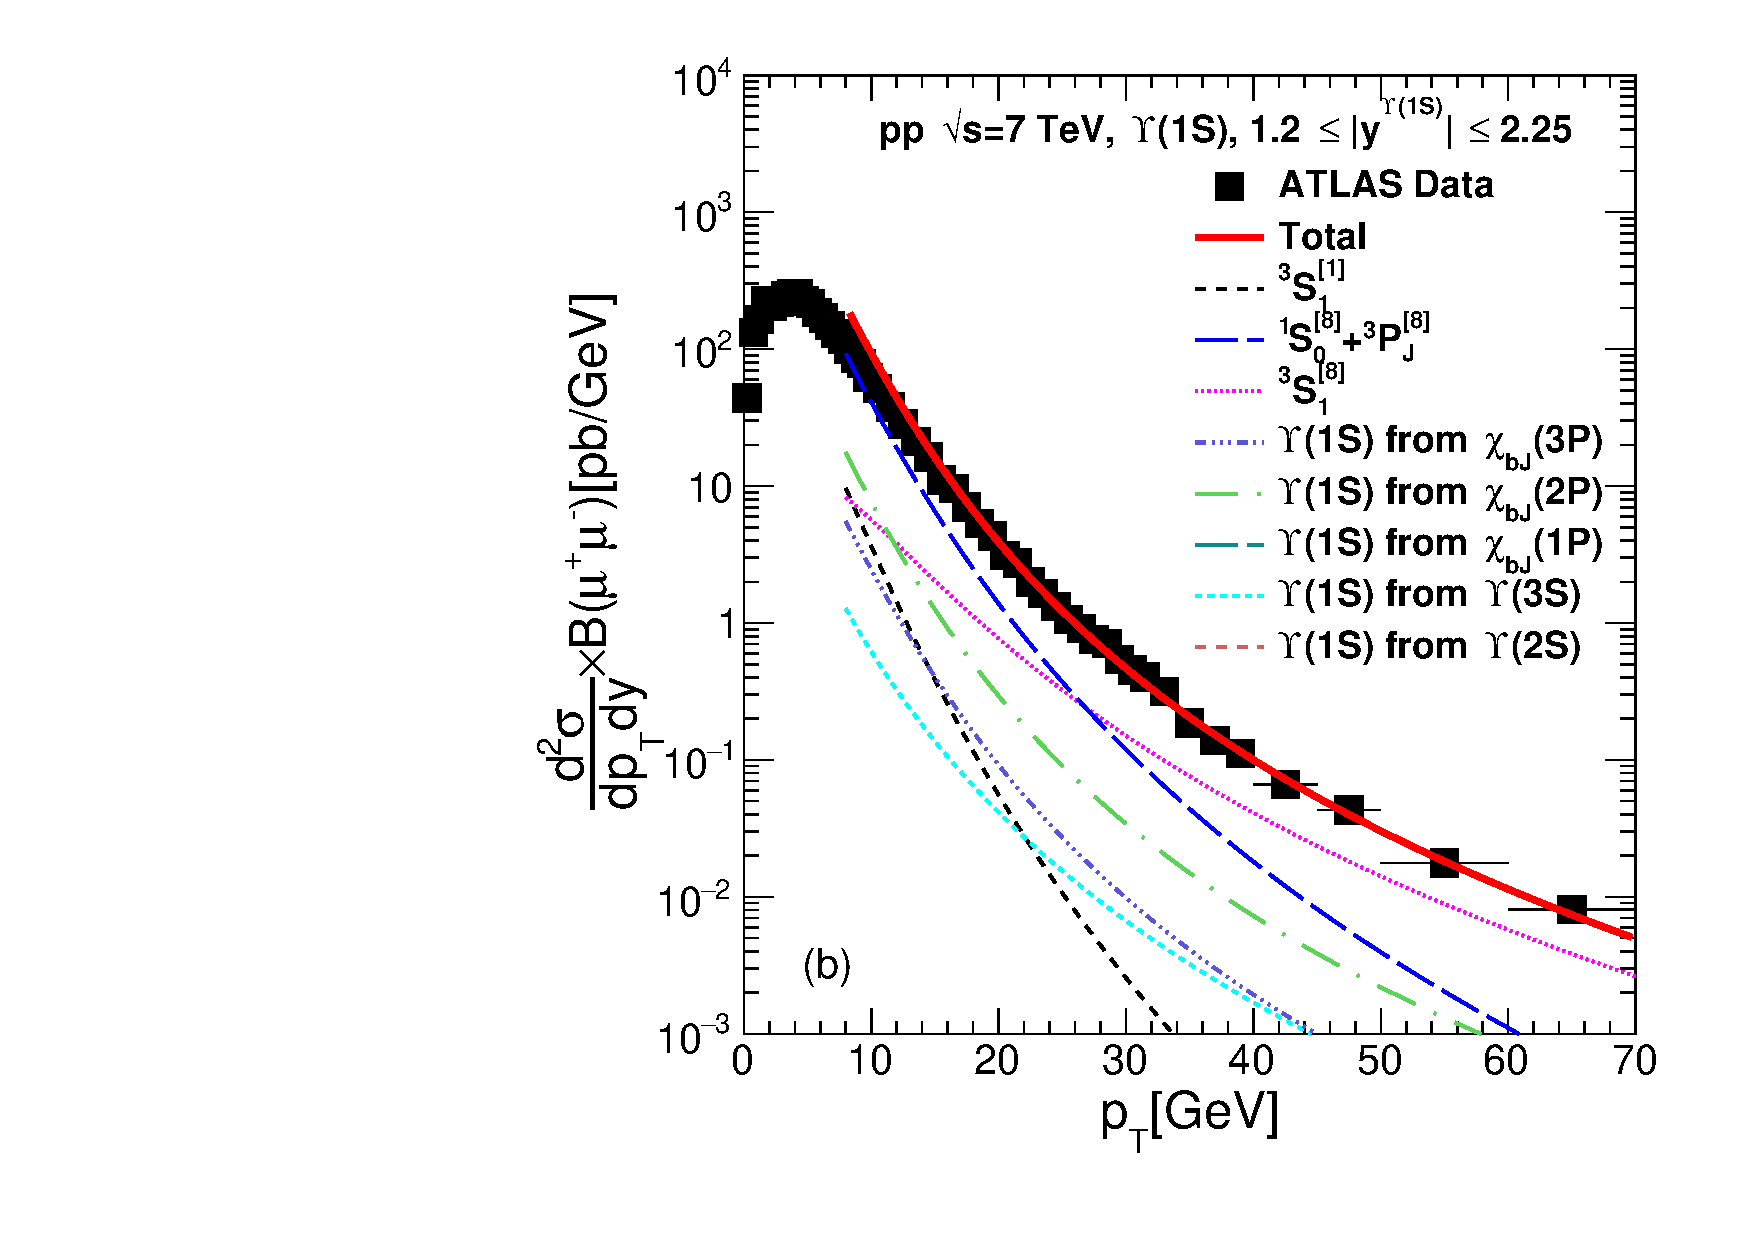
\includegraphics[width=0.49\textwidth]{Figures/NRQCD_Beauty/Fig7b_ATLAS_D2NDPtDy_Y1S_Y12225_Pt.pdf}
  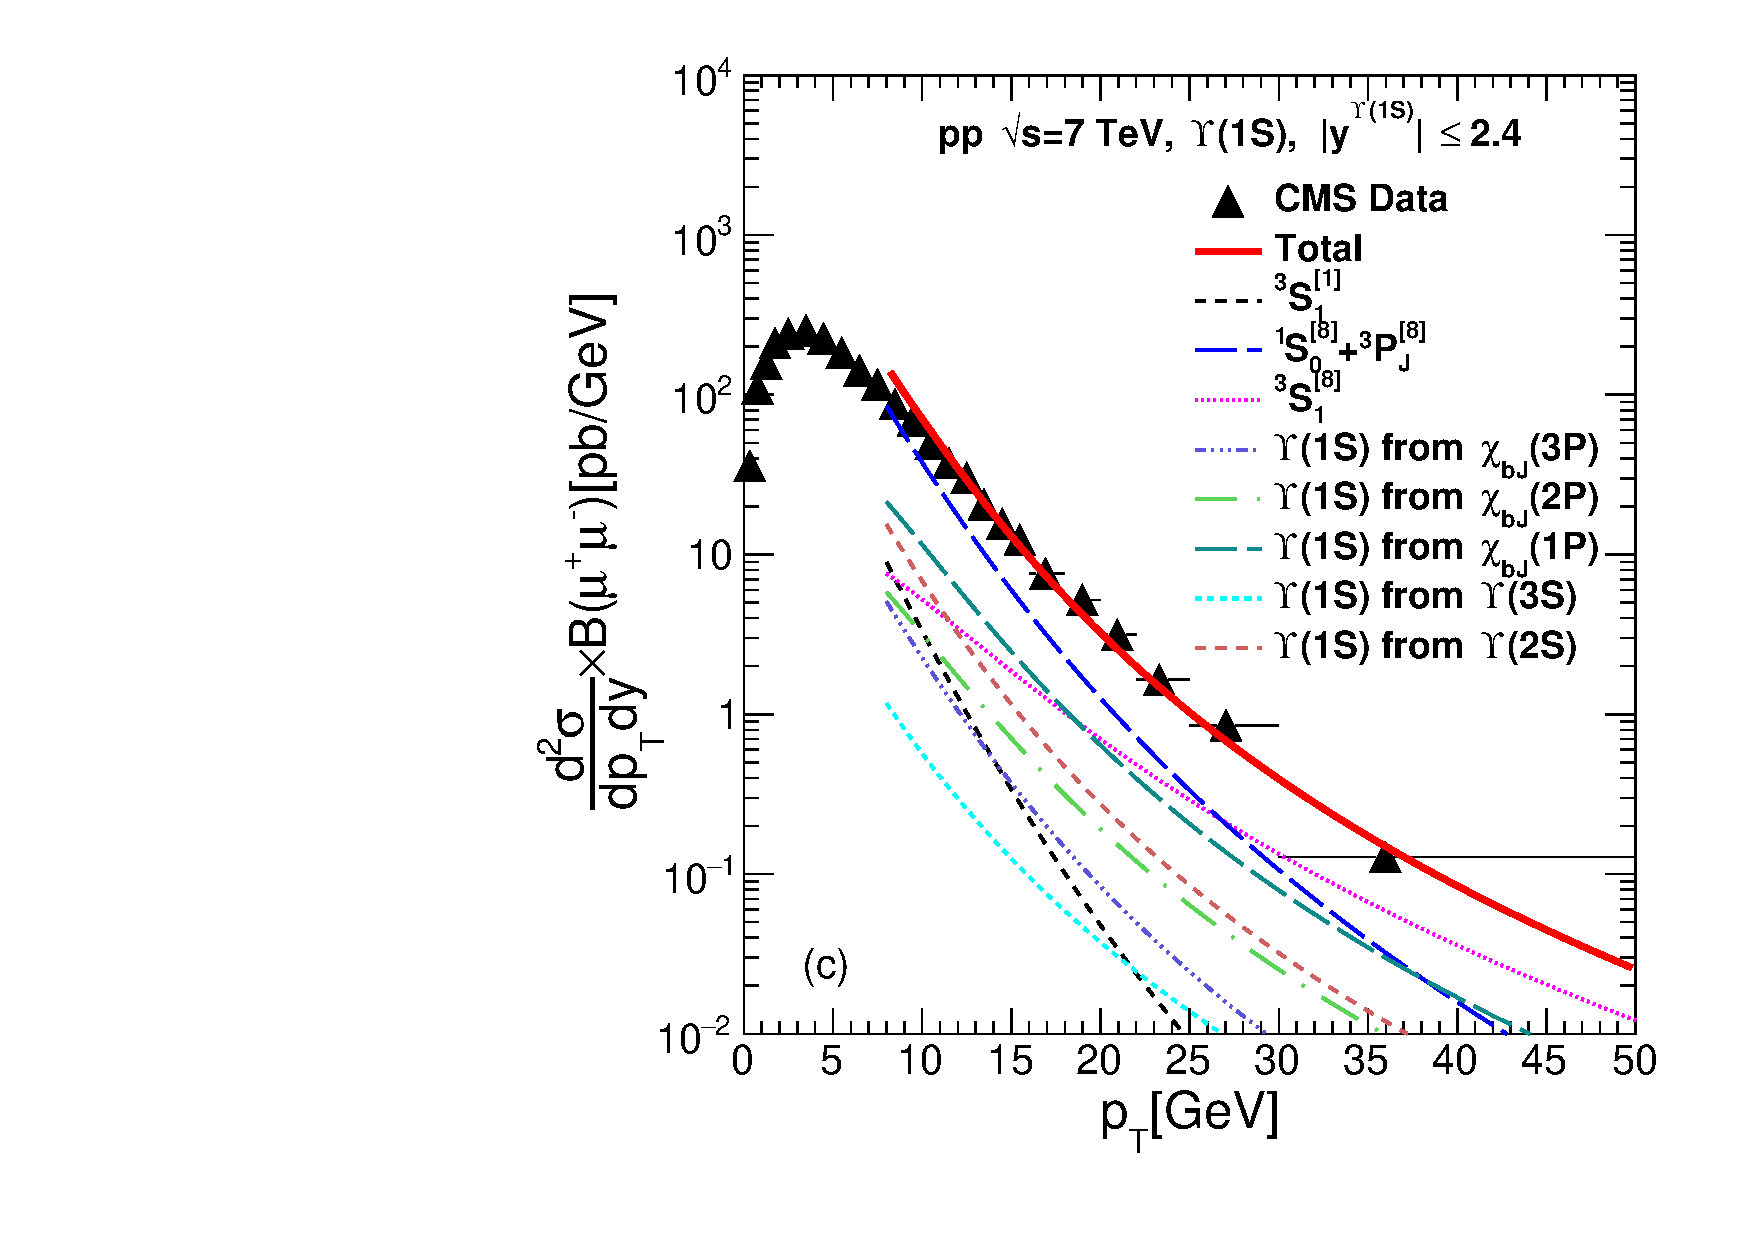
\includegraphics[width=0.49\textwidth]{Figures/NRQCD_Beauty/Fig7c_CMS_D2NDPtDy_Y1S_Y0024_Pt.pdf}
  \caption{\small{The NRQCD calculations of production cross-section of $\Upsilon$(1S) in p+p collisions at 
      $\sqrt{s}$ = 7 TeV in central and forward rapidities, as a function of transverse momentum compared 
      with the measured data at ATLAS~\cite{Aad:2012dlq} and CMS~\cite{Chatrchyan:2013yna} experiments.}}
  %   The LDMEs are obtained by a combined fit of the CMS and ATLAS data.}
  \label{Fig:SigmaY1SATLAS7TEV}
\end{figure}

\begin{figure}
  %width=0.8\textwidth,natwidth=610,natheight=642
  \centering
  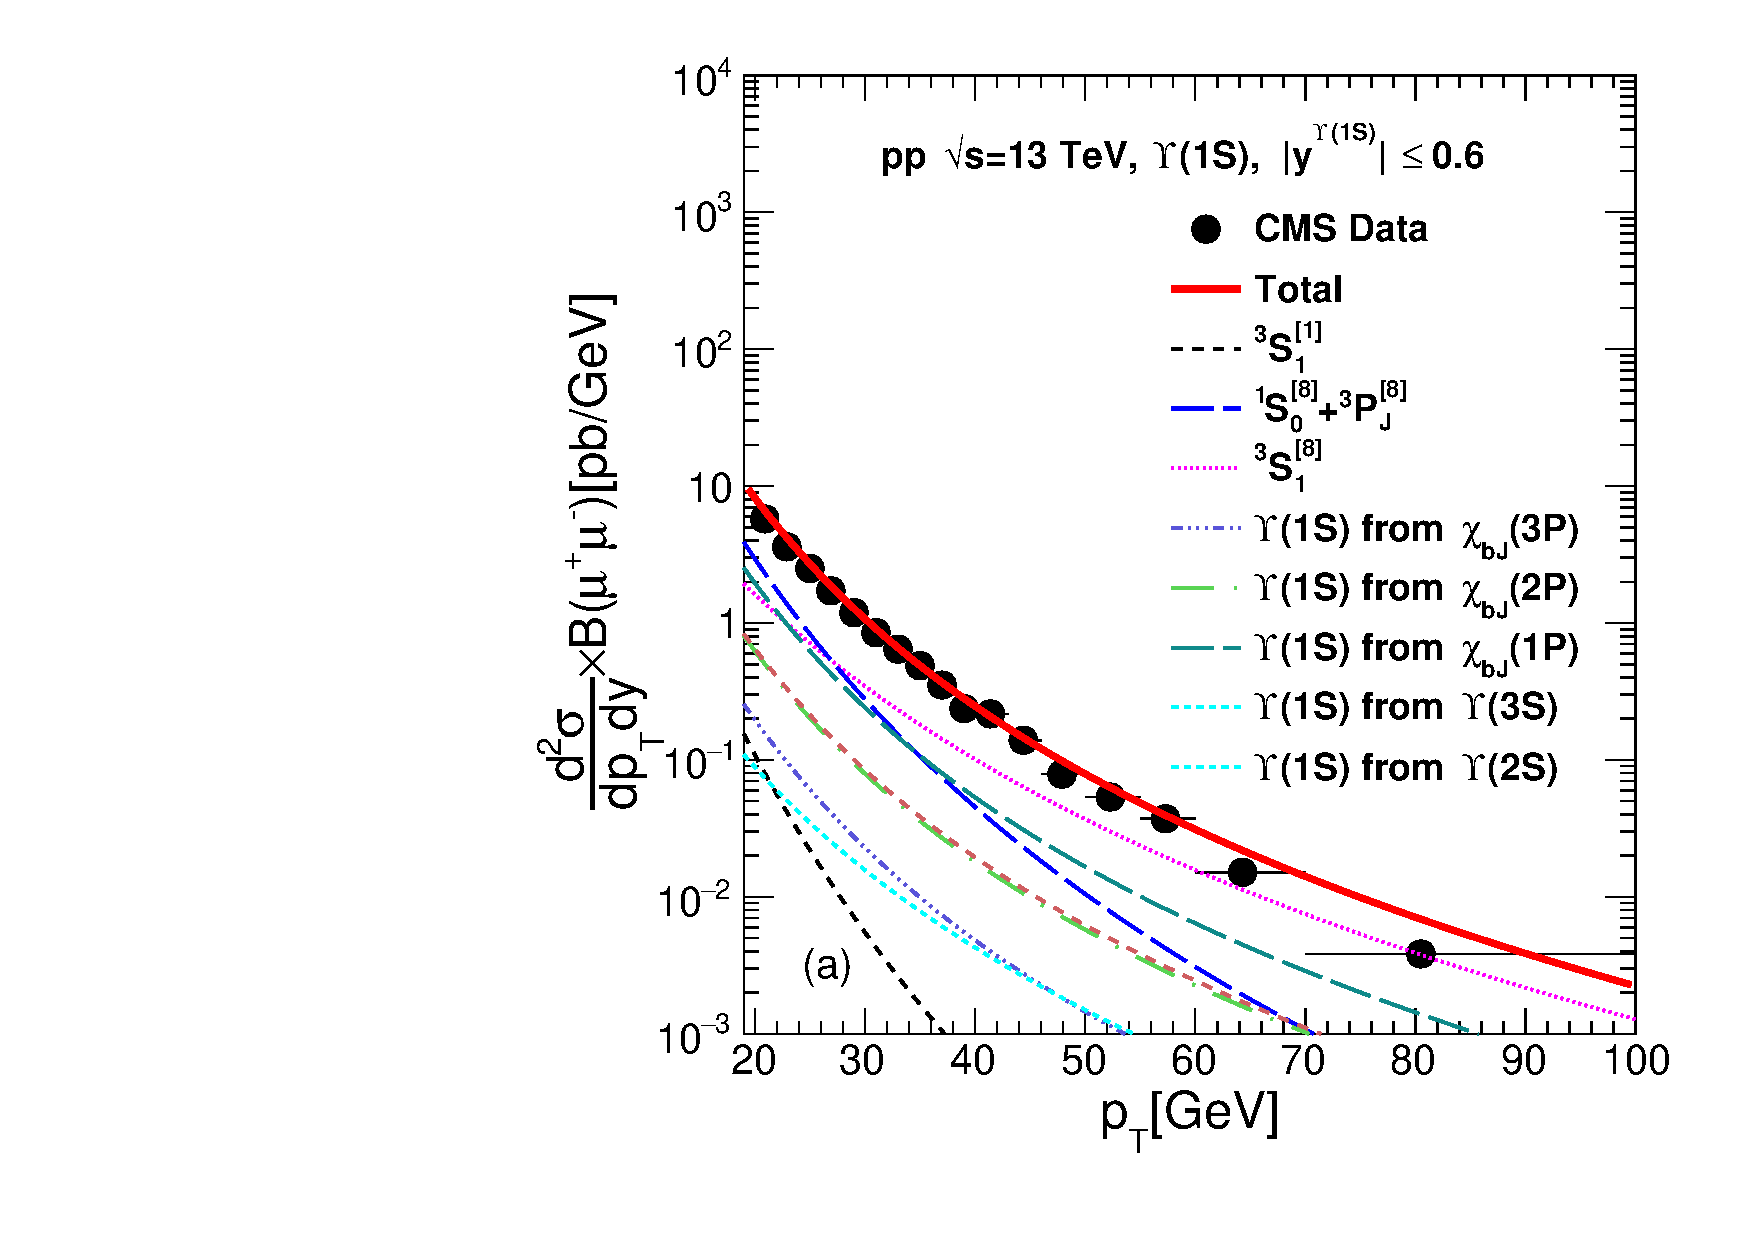
\includegraphics[width=0.49\textwidth]{Figures/NRQCD_Beauty/Fig8a_CMS_D2NDPtDy_Y1S_13TeV_Y0006_Pt.pdf}
  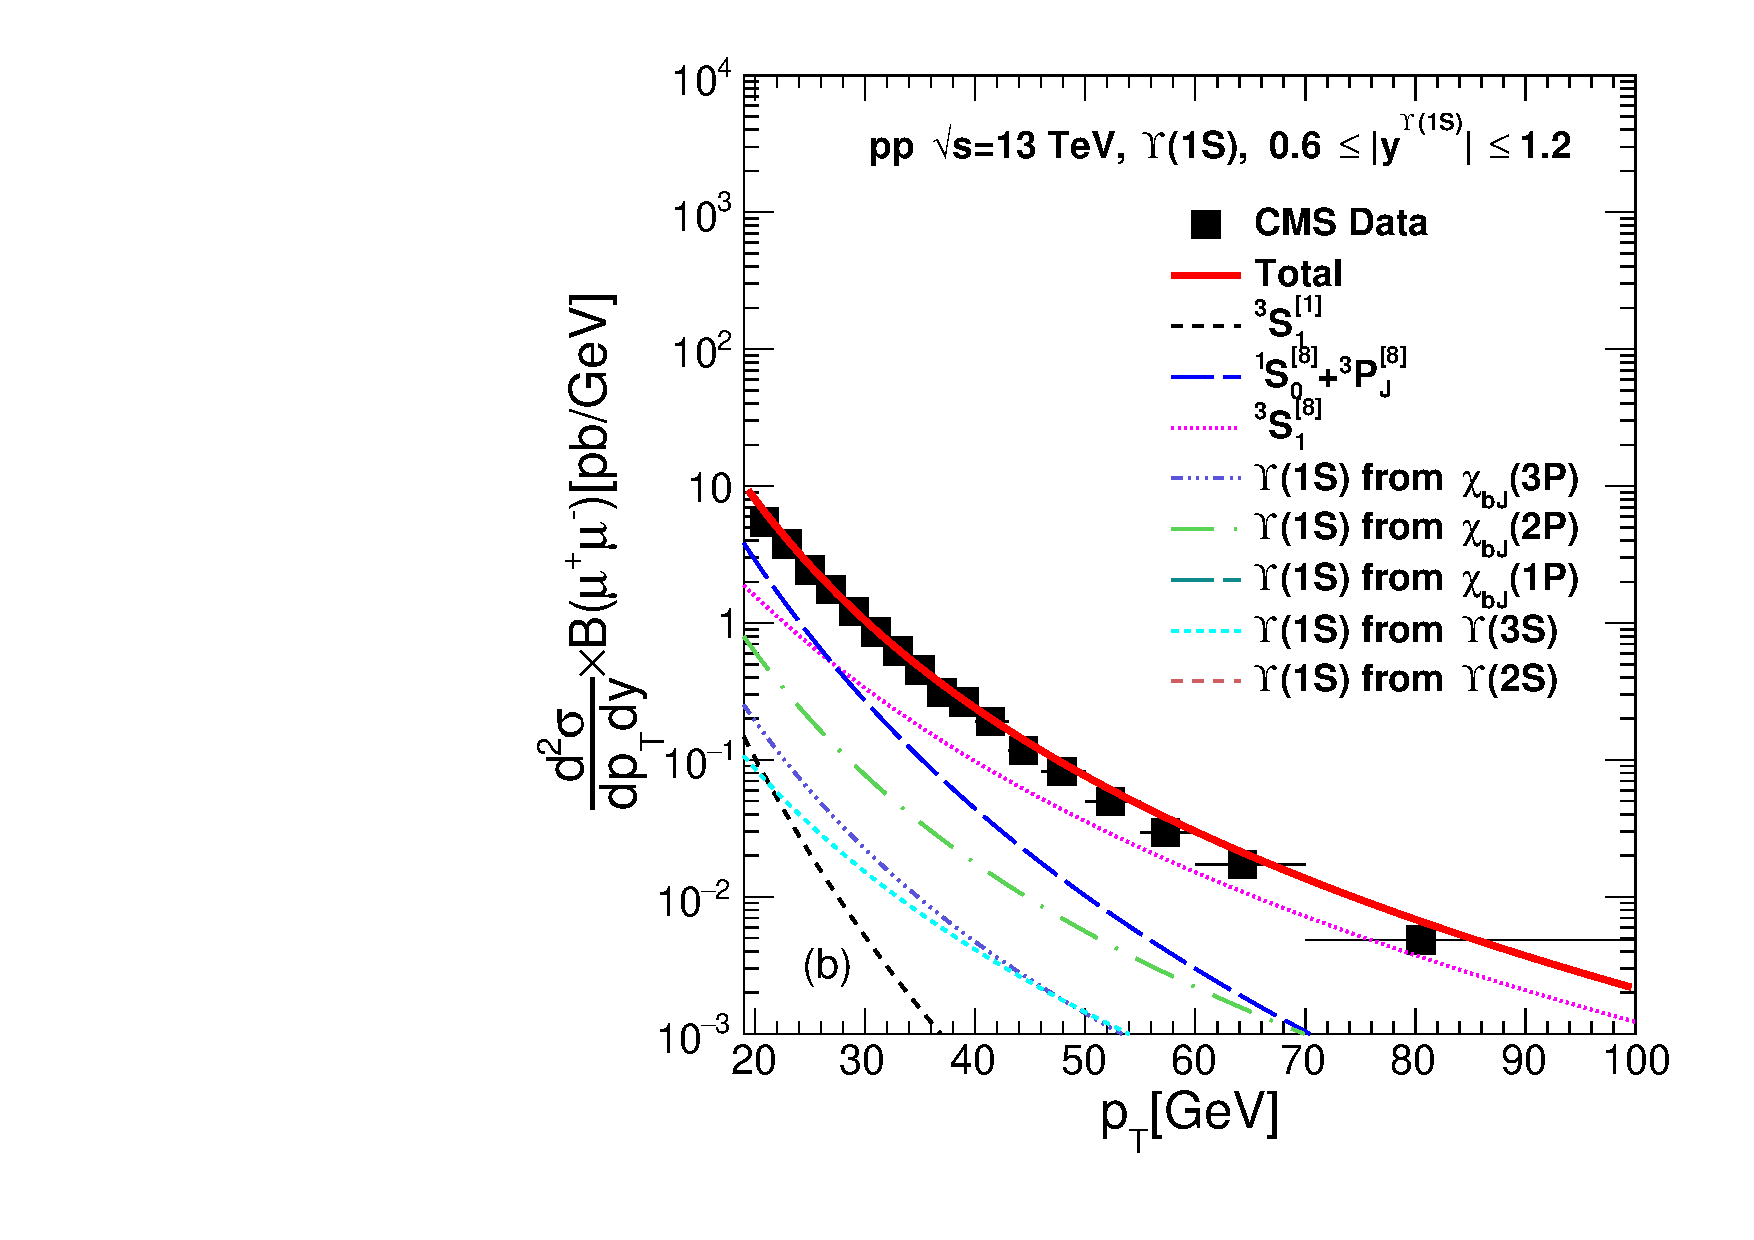
\includegraphics[width=0.49\textwidth]{Figures/NRQCD_Beauty/Fig8b_CMS_D2NDPtDy_Y1S_13TeV_Y0612_Pt.pdf} 
  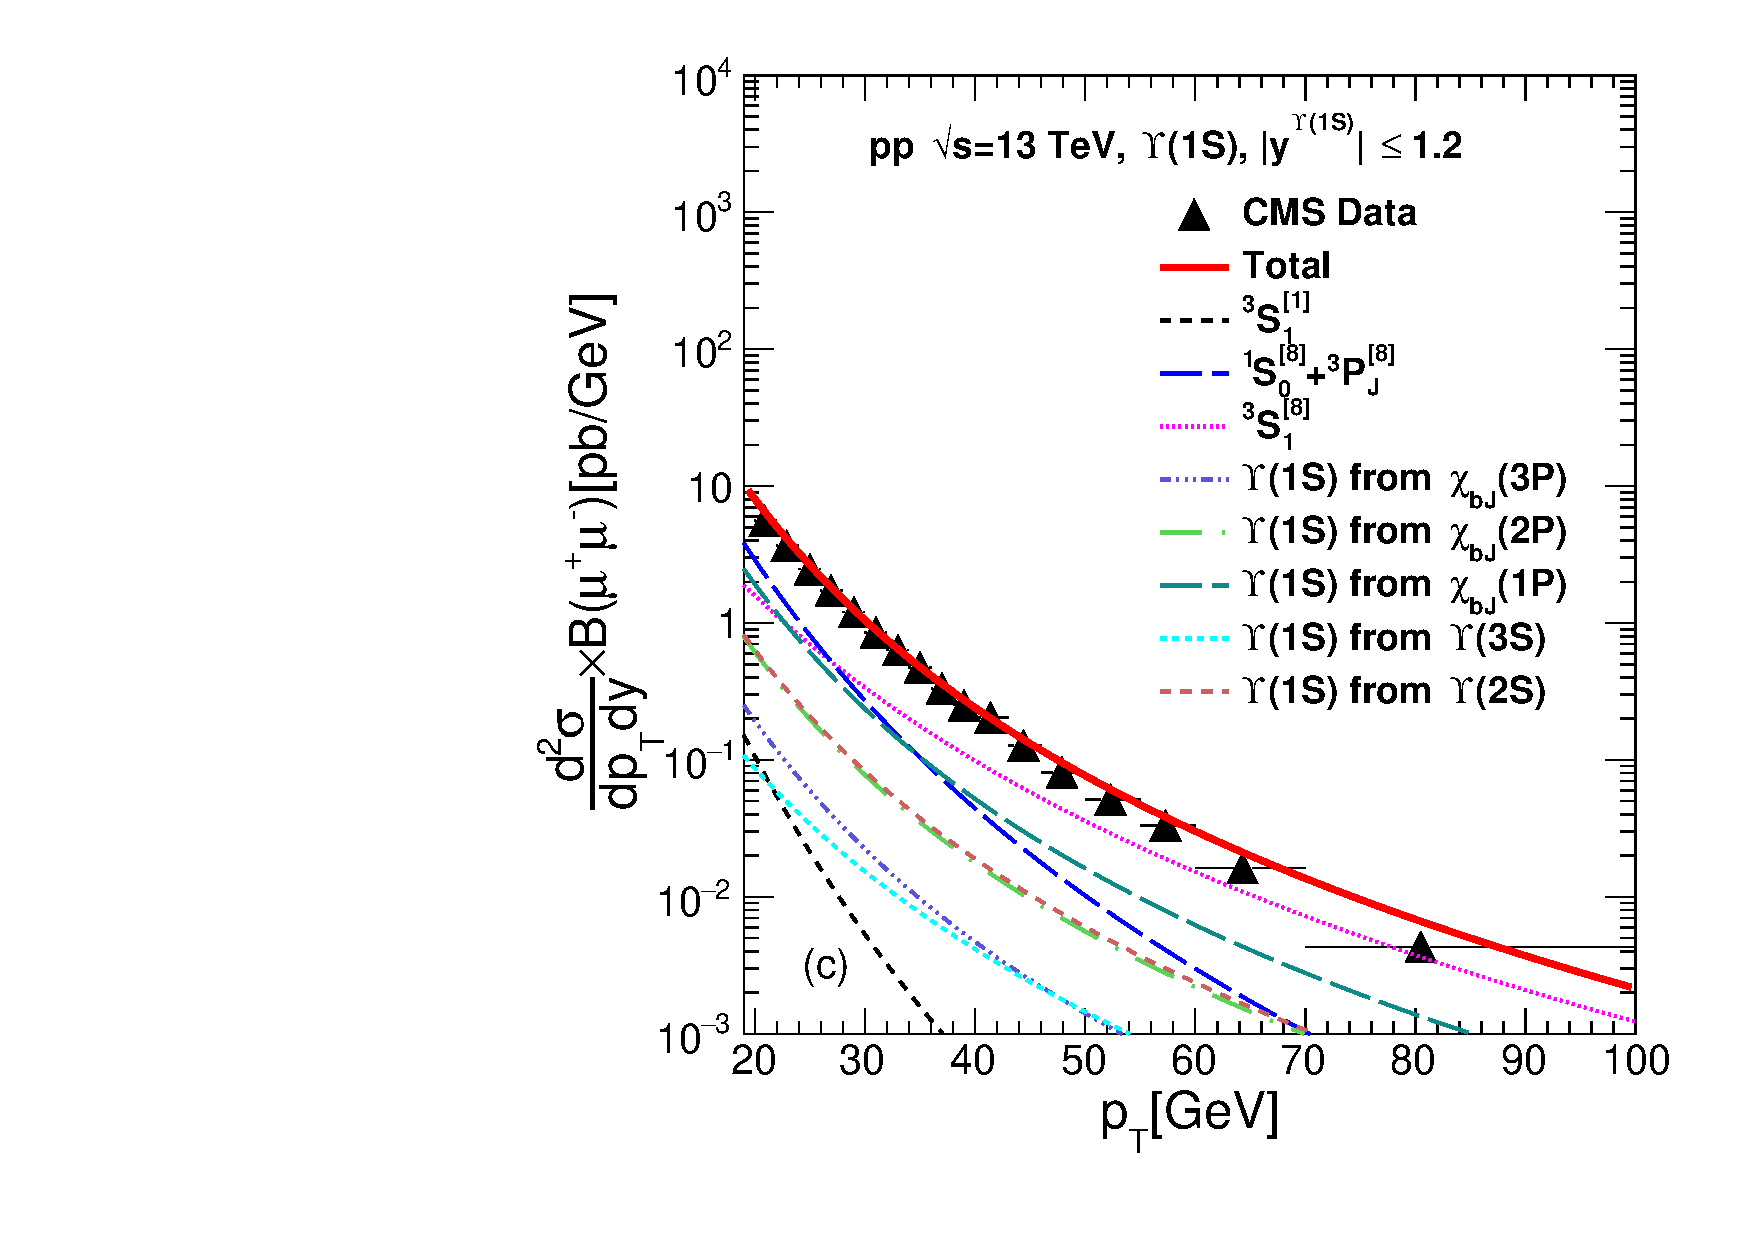
\includegraphics[width=0.49\textwidth]{Figures/NRQCD_Beauty/Fig8c_CMS_D2NDPtDy_Y1S_13TeV_Y0012_Pt.pdf}
  \caption{\small{The NRQCD calculations of production cross-section of $\Upsilon$(1S) in p+p collisions at 
      $\sqrt{s}$ = 13 TeV in central and forward rapidities, as a function of transverse momentum compared with the measured data 
      at CMS~\cite{Sirunyan:2017qdw} experiment. }}
  %   The LDMEs are obtained by a combined fit of the CMS and ATLAS data.}
  \label{Fig:SigmaY1SCMS13TeV}
\end{figure}

\paragraph{Results and discussions}
\label{sec:results}
%\subsection*{$\Upsilon$(3S)}
%We first start with the production of $\Upsilon$(3S), which being one of the highest bound state in
%the $b{\bar b}$ spectrum has feed down contributions only from $\chi_{b}$(3P).
We first start with the production of $\Upsilon$(3S) which has feed down contributions
only from $\chi_{b}$(3P).
As described, the expressions and the values for the 
colour-singlet elements can be obtained by solving the non-relativistic 
wavefunctions~\cite{Cho:1995vh}. 
The CO LDMEs on the other hand, cannot be connected to the non-relativistic
wavefunctions of $b \bar b$. 
%The reason being they involve a higher Fock state.
The measured data sets from different experimental collaborations are thus used to constrain them.
%For the present analysis on $\Upsilon$(3S), we make use of the datasets listed
%in the Table~\ref{DataY3S}.

Figure~\ref{Fig:SigmaY3SCMS} shows the NRQCD calculations of production cross-section of 
$\Upsilon$(3S) in p+p collisions as a function of transverse momentum compared with the 
measured data in CMS~\cite{Khachatryan:2015qpa} and ATLAS~\cite{Aad:2012dlq} 
detectors at LHC in central rapidities. In Figure~\ref{Fig:SigmaY3SCMS_forwardRap},
similar comparisons have been shown with data for $1.2<|y|<2.25$ and $|y|<2.4$
measured at ATLAS~\cite{Aad:2012dlq} and CMS~\cite{Chatrchyan:2013yna} detectors 
respectively. Figure~\ref{Fig:SigmaY3SCMS13TeV} corresponds to CMS ~\cite{Sirunyan:2017qdw}
measurements at $\sqrt{s}=13$ TeV for rapidities, $|y|<0.6$, $0.6<|y|<1.2$ and $|y|<1.2$, whereas in 
Figure~\ref{Fig:SigmaY3SCDF} we have used measurements from CDF~\cite{Acosta:2001gv}
collaboration in p +{$\bar {\rm p}$} at $\sqrt{s}=1.8$ TeV with $|y|<0.4$ as well as
that from LHCb ~\cite{LHCb:2012aa}
collaboration in p+p collisions at $\sqrt{s}=7$ TeV with rapidities $2.0<y<2.5$.
The LDMEs are obtained by a combined fit using all the aforesaid datasets.
The $\chi^2$/ndof is $\sim 4 $ for the combined fitting.

Table~\ref{LDMEsY3S} contains LDMEs for $\Upsilon$(3S) extracted in present analysis
in comparison with different other results. Our result for the matrix element $M_L(b\bar{b}([^3S_1]_8))$
shows a close proximity with LO analysis of Ref.~\cite{Brateen:PRD2001,Sharma:2012dy}, the errors being improved
considerably.
In our work, we have considered a linear combination of the other two colour octet 
LDMEs in the form of $\frac{M_{L}([^1S_0]_{8})}{5}+\frac{3M_{L}([^3P_0]_{8})}{m_b^2}$, same as that
done in Ref.~\cite{Sharma:2012dy}.
%Our result shows higher value, the error however
%got reduced significantly as compared to the previous LO study ($\approx 300\%$).
There have been different ways to treat the colour octet LDMEs in the literature.
In Ref.~\cite{Domenech:2000ri}, 
the authors have taken this combination as $M_{L}([^1S_0]_{8})+\frac{5M_{L}([^3P_0]_{8})}{m_b^2}$.
In Ref.~\cite{Brateen:PRD2001}, these two matrix elements,
$M_{L}([^1S_0]_{8})$ and $\frac{5M_{L}([^3P_0]_{8})}{m_b^2}$
have been extracted separately using two different PDFs. In each case however, they have extracted
either of the two parameters considering the other to be vanishing.
The work in Ref.~\cite{Gong:2010bk} concentrates only on S-wave colour states.
In Refs.~\cite{Gong:2013qka,Feng:2015wka},
the parameters, $M_{L}([^1S_0]_{8})$ and $\frac{M_{L}([^3P_0]_{8})}{m_b^2}$ have been extracted
separately altogether. On the other hand in Ref.~\cite{Han:2014kxa}, the authors have
considered different combinations of 
colour octet states to fit with the experimental data with NRQCD at LO and NLO using 
CTEQ6L1 and CTEQ6M PDFs respectively with $m_b$=4.75 GeV and $[^3S_1]_1$=3.54 GeV$^3$.
Their extracted parameters are,
\begin{eqnarray}
  \nonumber
  M_{0,r_0}~=~[^1S_0]_8+\frac{r_0}{m_b^2}[^3P_0]_8~=~0.0283\pm 0.0007{\rm \,\, GeV^3} \nonumber \\
  M_{1,r_1}~=~[^3S_1]_8+\frac{r_1}{m_b^2}[^3P_0]_8~=~0.0083\pm 0.0002{\rm \,\,GeV^3} 
\end{eqnarray}
with $r_0$=3.8 and $r_1$=-0.52 GeV$^2$.

After fixing the $\Upsilon$(3S) yield, we next consider $\Upsilon$(2S) production 
that has feed down contributions from $\Upsilon$(3S), $\chi_b(2P)$ and $\chi_b(2P)$ states
along with the direct production. The corresponding
branching fractions for the feed down sectors are given in
Table~\ref{BRUpsilon}. We have used our extracted values of the $\Upsilon$(3S) LDMEs
for the feed down contributions from the $\Upsilon$(3S). To include the $\chi_b(nP)$ states feed down
LDMEs are obtained from Ref.~\cite{Sharma:2012dy,Feng:2015wka}.
%The CS contributions are calculated in a similar manner.
%For the CO LDMEs,
%we use the datasets given in Table~\ref{DataY2S},
%\begin{table}[h]
%\centering
%\caption{Datasets from different experimental collaborations used to constrain 
%the NRQCD CO LDMEs for $\Upsilon$(2S).}
%\begin{tabular}{ccc}
%\hline
%\hline
%& & \\ 
%Experiments & $\sqrt{s}$ & rapidity \\
%\hline 
%& & \\
%CMS & 7 TeV & $|y| <$2.4 \\
%%& & $|y|< $2.4 \\
%ATLAS & 7 TeV & $|y| <$1.2 \\
%& & 1.2 $< |y| <$ 2.25 \\
%CMS & 13 TeV & $|y| <$0.6 \\
%& & 0.6$< |y|< $1.2 \\
%& & $|y| <$ 1.2 \\
%%CDF & 1.8 TeV & $|y| <$0.4 \\
%%LHCb& 7 TeV & 2.0$< |y|< $2.4 \\ \\
% \hline
% \hline
%\end{tabular}
%\label{DataY2S}
%\end{table}

In Fig~\ref{Fig:SigmaY2SATLAS}, we have shown our NRQCD predictions of production
cross-sections for $\Upsilon$(2S) in p+p collisions as functions of 
$p_T$ along with the measured data in CMS~\cite{Chatrchyan:2013yna} and ATLAS~\cite{Aad:2012dlq}
detectors at central and forward rapidities. All the contributions
alongwith feed down ones are displayed separately. Fig.~\ref{Fig:SigmaY2SCMS13TeV} describes 
the same alongwith the data from CMS detector at 13 TeV for 
both central and forward rapidities. Our results of CO LDMEs for 
$\Upsilon$(2S) have been given in Table~\ref{LDMEsY2S} along with existing results
from different other groups.
Our value for $M_L(b\bar{b}([^3S_1]_8 \rightarrow \Upsilon(2S))$ is in agreement with the
values from other groups also $M_L(b\bar{b}([^1S_0]_8,[^3P_0]_8 \rightarrow \Upsilon(2S))$
does not have negative value (which is unphysical) unlike some other groups.
%We have considered a minimum $p_T$ value of 8 GeV except for CMS 13 TeV datasets for the fit.
%Though the individual values of the CO LDMEs are larger compared to the previous
%estimates, the errors are considerably reduced now.
The inclusion of 13 TeV data along with the incorporation of feed down from $\chi_{b}$(3P),
is expected to give better constrains of LDMEs.

In~\cite{Domenech:2000ri,Brateen:PRD2001,Sharma:2012dy,Gong:2013qka,Feng:2015wka,Han:2014kxa}, 
authors have considered different combinations of
CO LDMEs that has already been described. In Ref.~\cite{Han:2014kxa}, the extracted 
parameters for $\Upsilon$(2S) are,
\begin{eqnarray}
  \nonumber
  M_{0,r_0}=0.0607\pm0.0108 \,\,{\rm GeV^3}\\ \nonumber
  M_{1,r_1}=0.0108\pm0.0020 \,\,{\rm GeV^3}
\end{eqnarray}
with $[3S_1]_1$=4.63 GeV$^3$ and the values of $r_0$ and $r_1$ are same as given before.
The $\chi^2$/ndof for the 
combined fit in our analysis is $\sim$ 2.7.

\begin{table*}
  \centering
  \caption{Comparison of CS elements and CO LDMEs extracted from fitting with experimental data
    using NRQCD formalism for $\Upsilon$(2S).}
  \footnotesize
  %\begin{tabular}{ccccccc}
  \begin{tabular*}{\textwidth}{@{\extracolsep{\fill}}lrrrrrl@{}}
    \hline
    \hline
    %& & & & & & \\
    Ref. (LO/NLO) & PDF & $m_b$ & $M_L(b\bar{b}([^3S_1]_1$ & $M_L(b\bar{b}([^3S_1]_8$ & 
    $M_L(b\bar{b}([^1S_0]_8$, & $p_T$-cut \\
    & & & $\rightarrow\Upsilon(2S)$ & $\rightarrow\Upsilon(2S)$ & $[^3P_0]_8\rightarrow\Upsilon(2S)$ & \\
    & & (GeV) & $({\rm GeV^3})$ & $({\rm GeV^3})$ & $({\rm GeV^3})$ & GeV/$c$ \\
    %& & & & & & \\
    \hline
    \hline
    & & & & & & \\
    present (LO) & CT18 &4.88 &4.5 &0.0391$\pm$0.0016 & 0.0477$\pm$0.0019 & 8   \\
    %& (LO) & & & & & \\
    %\hline
    & & & & & & \\
    \cite{Domenech:2000ri} (LO) & CTEQ4L & 4.88 & 5.01 & 0.040$\pm$0.029 & 0 & 2 \\
    & & & & 0.073$\pm$0.018 & 0 & 4 \\
    & & & & 0.103$\pm$0.027 & 0 & 8 \\
    & & & & & & \\
    %\hline
    %& & & & & & \\
    \cite{Brateen:PRD2001} (LO) & CTEQ5L & 4.77 & 5.0$\pm$0.7 & 0.180$\pm$0.056 & -0.102$\pm$0.097 & 8 \\
    & & & & 0.172$\pm$0.050 & -0.106$\pm$0.102 & \\
    & & & & & & \\
    & MRSTLO & 4.77 & 5.0$\pm$0.7 & 0.196$\pm$0.063 & -0.087$\pm$0.111 & 8 \\
    & & & & 0.190$\pm$0.056 & -0.089$\pm$0.117 & \\
    & & & & & & \\
    %\hline
    %& & & & & & \\
    \cite{Sharma:2012dy} (LO) & MSTW08LO & 4.88 & 4.5 & 0.0224$\pm$0.0200 & -0.0067$\pm$0.0084 & -  \\
    %& (LO) & & & & & \\
    %\hline
    & & & & & & \\
    \cite{Gong:2013qka} (NLO) & CTEQ6M & 5.01 & 4.63 & 0.0030$\pm$0.0078 & 0.0075$\pm$0.0217 & 8 \\
    %& (NLO) & & & & & \\
    %\hline
    & & & & & & \\
    \cite{Feng:2015wka} (NLO) & CTEQ6M & 5.01 & 4.63 & 0.0222$\pm$0.0024 & -0.0003$\pm$0.0203 & 8 \\
    %& (NLO) & & & & & \\
    \hline
    \hline
  \end{tabular*}
  \label{LDMEsY2S}
\end{table*}
\normalsize
Having completed $\Upsilon$(3S) and $\Upsilon$(2S) parts, we now move on to explore $\Upsilon$(1S). 
Alongwith the direct yield, it has feed down contributions from higher
S-wave states like $\Upsilon$(3S) and $\Upsilon$(2S), as well as P-wave states like $\chi_b$(3P), $\chi_b$(2P)
and $\chi_b$(1P). The associated branching functions are provided in Table~\ref{BRUpsilon}.
The extracted CO-LDMEs for $\Upsilon$(3S) and $\Upsilon$(2S) are used for feed down contributions,
whereas the LDMEs for the $\chi_b$(nP) states have been taken from Ref.~\cite{Sharma:2012dy,Feng:2015wka}
for this present case study.
In Fig.~\ref{Fig:SigmaY1SATLAS7TEV}, we have displayed our NRQCD calculation of production cross-section 
of $\Upsilon$(1S) as function of $p_T$ along with the experimental measurements by ATLAS and
CMS at $\sqrt{s}$=7 TeV in central rapidities.
%Fig.~\ref{Fig:SigmaY1SATLAS7TEV} shows the same in comparison
%with ATLAS measurements at both central and forward rapidities.
Finally in Fig.~\ref{Fig:SigmaY1SCMS13TeV}, we present our results along with
the CMS measurements at 13 TeV with all the components separately to signify their relative
contributions. 
\begin{table*}
  \centering
  \caption{Comparison of CS elements and CO LDMEs extracted from fitting with experimental data
    using NRQCD formalism for $\Upsilon$(1S).}
  \footnotesize
  %\begin{tabular}{ccccccc}
  \begin{tabular*}{\textwidth}{@{\extracolsep{\fill}}lrrrrrl@{}}
    \hline
    \hline
    %& & & & & & \\
    Ref. (LO/NLO) & PDF & $m_b$ & $M_L(b\bar{b}([^3S_1]_1$ & $M_L(b\bar{b}([^3S_1]_8$ & 
    $M_L(b\bar{b}([^1S_0]_8$, & $p_T$-cut \\
    & & & $\rightarrow\Upsilon(1S)$ & $\rightarrow\Upsilon(1S)$ & $[^3P_0]_8\rightarrow\Upsilon(1S)$ & \\
    & & (GeV) & $({\rm GeV^3})$ & $({\rm GeV^3})$ & $({\rm GeV^3})$ & GeV/$c$ \\
    %& & & & & & \\
    \hline
    \hline
    & & & & & & \\
    present (LO) & CT18 &4.88 &10.9 &0.0601$\pm$0.0017 & 0.0647$\pm$0.0016 & 8   \\
    %& (LO) & & & & & \\
    %\hline
    & & & & & & \\
    \cite{Domenech:2000ri} (LO) & CTEQ4L & 4.88 & 11.1 & 0.077$\pm$0.017 & 0 & 2 \\
    & & & & 0.087$\pm$0.016 & 0 & 4 \\
    & & & & 0.106$\pm$0.013 & 0 & 8 \\
    & & & & & & \\
    %\hline
    %& & & & & & \\
    \cite{Brateen:PRD2001} (LO) & CTEQ5L & 4.77 & 12.8$\pm$1.6 & 0.116$\pm$0.027 & 0.109$\pm$0.062 & 8 \\
    & & & & 0.124$\pm$0.025 & 0.111$\pm$0.065 & \\
    & & & & & & \\
    & MRSTLO & 4.77 & 12.8$\pm$1.6 & 0.117$\pm$0.030 & 0.181$\pm$0.072 & 8 \\
    & & & & 0.130$\pm$0.028 & 0.186$\pm$0.075 & \\
    & & & & & & \\
    %\hline
    %& & & & & & \\
    \cite{Sharma:2012dy} (LO) & MSTW08LO & 4.88 & 10.9 & 0.0477$\pm$0.0334 & 0.0121$\pm$0.0400 & -  \\
    %& (LO) & & & & & \\
    %\hline
    & & & & & & \\
    \cite{Gong:2013qka} (NLO) & CTEQ6M & 4.75 & 9.282 & -0.0041$\pm$0.0024 & 0.0780$\pm$0.0043 & 8 \\
    %& (NLO) & & & & & \\
    %\hline
    & & & & & & \\
    \cite{Feng:2015wka} (NLO) & CTEQ6M & PDG & 9.282 & 0.0061$\pm$0.0024 & 0.0895$\pm$0.0248 & 8 \\
    %& (NLO) & & & & & \\
    \hline
    \hline
  \end{tabular*}
  \label{LDMEsY1S}
\end{table*}
\normalsize

Table~\ref{LDMEsY1S} shows our results for $\Upsilon$(1S) parameters along with
the results from different groups. The individual values of LDMEs are in agreement with
the values from previous works but with considerable reduction in 
errors upon inclusion of 13 TeV data sets from CMS.
The values of the parameters $M_{0,r_0}$ and $M_{1,r_1}$ extracted in Ref.~\cite{Han:2014kxa} are,
\begin{eqnarray}
  \nonumber
  M_{0,r_0}=0.1370\pm0.0111 \, {\rm GeV^3},\\ \nonumber
  M_{1,r_1}=0.0117\pm0.0002 \, {\rm GeV^3}
\end{eqnarray}
with $[3S_1]_1$=9.28 GeV$^3$ keeping $r_0$ and $r_1$ same as given before.
%The $\chi^2$/ndof for our analysis of $\Upsilon$(1S) is $\sim$ 1.7.

\paragraph{Summary}
\label{sec:summary}
%We have calculated the differential production cross-section of $\Upsilon$(3S) meson
%as a function of transverse momentum. The data from LHC experiments are used to 
%obtain the values of colour octet LDMEs. We plan to present a rigorous study of 
%production of all states of bottomonia at LHC energies using NRQCD.
%The re-evaluation of all LDMEs required for bottomonia production is in progress using 
%latest data from LHC. 
%{\colour{red} (can be modified)   
We have presented NRQCD calculations for the differential production 
cross-sections of $\Upsilon$ states in  p+p collisions.  Measured transverse momentum
distributions of $\Upsilon$(3S), 
$\Upsilon$(2S) and $\Upsilon$(1S) in p +{$\bar {\rm p}$} collisions at $\sqrt{s}=$ 1.8 TeV and in 
p+p collisions at 7 TeV and 13 TeV are used to constrain the LDMEs. All the relevant feeddown
contributions from higher mass states including the $\chi_{b}$(3P) are taken in to account.
The calculations for  $\Upsilon$(3S), $\Upsilon$(2S) and $\Upsilon$(1S) are compared with 
the measured data at Tevatron and LHC. The formalism provides  very good description of the data in 
large transverse momentum range at different collision energy. 
%The values of LDMEs are used to predict the charmonia cross-sections in p+p collisions 
%at 13 and 5 TeV in kinematic bins relevant for LHC detectors. 
We compare the LDMEs for bottomonia obtained in this analysis with the results from earlier works.
At high $p_T$, the colour singlet contribution is very small and LHC data in large $p_T$ range 
help to constrain the relative contributions of different colour octet contributions.
For $\Upsilon$ states at high  $p_T$, the contribution of the  
$M_{L}(b\barb([^3S_1]_{8}\rightarrow \Upsilon(nS)))$ is highest which is opposite to the charmonia 
case where the contribution for the combination of  $M_{L}(c\barc([^1S_0]_{8},[^3P_0]_{8})\rightarrow \psi)$ 
is more~\cite{Kumar:2016ojy}.
%The high energy LHC data require a smaller value of the LDME $M_{L}(c\barc([^3S_1]_{8}\rightarrow \psi))$ 
%and a larger value for the combination  $M_{L}(c\barc([^1S_0]_{8},[^3P_0]_{8})\rightarrow \psi)$ of LDMEs.   
In summary, we present a comprehensive lowest-order analysis of hadroproduction data of bottomonia 
states using the latest parton distribution functions and including very recent LHC data. The feed-down
contributions from all the $\chi_{b}$ states are included in the calculations. The values of relevant LDMEs
are extracted by doing a simultaneous fit of all the data sets. These values will be useful for predictions
of quarkonia cross-section and for the purpose of a comparison with those obtained using the NLO formulations.
%}


\section{Bottomonia production mechanism in heavy ion collisions}
\label{sec:Bottomonia_hi}

\subsection{Theory overview}

\subsubsection{Sequential suppression and lattice QCD}
{\color{red} This subsection will include the details of the model by Strickland et. al. This
reference have most of the details about the model~\cite{Mocsy:2013syh}}
              
              
\subsubsection{Effect of nuclear PDFs on quarkonium production in nucleus–nucleus collisions}
{\color{red} This subsection will include the details of the models which use nuclear PDFs for quarkonia production
like EPS19 or Color Glass Condensate modes. etc.~\cite{}. These effects are small for the Upsilon sector. }


\subsubsection{Collisional dissociation of quarkonia from final-state interactions}

{\color{black}
                              
                             
  
                              
  \paragraph{Modification of quarkonia in the presence of QGP}
  In the kinetic approach \cite{Thews:2000rj}, the proper time $\tau$ evolution of the quarkonia 
  population $N_{Q}$
  is given by the rate equation 
  
  \begin{equation}\label{eqkin}
    {dN_{Q} \over d\tau}  =  - \lambda_D  \rho_g N_{Q} + \lambda_F {N_{q \bar{q}}^{2} \over V(\tau)},
  \end{equation}
  where $V(\tau)$ is the volume of the deconfined spatial region and $N_{q \bar{q}}$ is the number of initial 
  heavy quark pairs produced per event depending on the centrality defined by the number of participants
  $N_{\rm part}$.
  The $\lambda_{D}$ is the dissociation rate obtained by the dissociation cross section averaged over 
  the momentum 
  distribution of gluons and $\lambda_{F}$ is the formation rate obtained by the formation cross section 
  averaged over the momentum distribution of heavy quark pair $q$ and $\bar{q}$. 
  $\rho_g$ is the density of thermal gluons.
  The number of quarkonia at freeze-out time $\tau_f$ is given by the solution of Eq.~(\ref{eqkin}),
  \begin{equation}
    N_{Q}(p_T) = S(p_T) \,N_{Q}^{\rm PbPb}(p_T)+N_{Q}^F(p_T).
    \label{eqbeta}
  \end{equation}
  Here $N_{Q}^{\rm PbPb}(p_T)$ is the number of initially-produced quarkonia (including shadowing)
  as a function of $p_T$ and $S(p_T)$ is their survival probability from gluon collisions at freeze-out, 
  \begin{equation}
    S(p_T) = \exp \left( {-\int_{\tau_0}^{\tau_f}f(\tau) \lambda_{\rm D}(T,p_T)\,\rho_g(T)\,d\tau} \right).
  \end{equation}
  The temperature $T(\tau)$ and the QGP fraction $f(\tau)$ evolve from initial time $\tau_0$ 
  to freeze-out time $\tau_f$ due to expansion of the QGP. The initial temperature and the 
  evolution is dependent on collision centrality $N_{\rm part}$.
  $N_{Q}^F(p_T)$ is the number of regenerated quarkonia per event,
  \begin{equation}
    N_{Q}^F(p_T)=S(p_T)N_{q \bar{q}}^{2} \int_{\tau_0}^{\tau_f}{{\lambda_{\mathrm{F}}(T,p_T) \over V(\tau)\,S(\tau,p_T)} d\tau}.
  \end{equation}
  The nuclear modification factor ($R_{AA}$) can be written as 
  \begin{equation}
    R_{AA}(p_T)=S(p_T) \, R(p_T) + \frac{N_{Q}^F(p_T)}{N_{Q}^{pp}(p_T)}.
    \label{raa}
  \end{equation}
  Here $R(p_T)$ is the shadowing factor.
  $R_{AA}$ as a function of collision centrality, including regeneration, is
  \begin{equation}
    R_{AA}(N_{\rm part}) = \frac{\int_{p_{T\,\rm cut}} N_{Q}^{pp}(p_T)S(p_T)\, R(p_T) dp_T}{\int_{p_{T\,\rm cut}} N_{Q}^{pp}(p_T) dp_T} + 
    \frac{\int_{p_{T\, \rm cut}} N_{Q}^F(p_T) dp_T}{\int_{p_{T\, \rm cut}} N_{Q}^{pp}(p_T) dp_T}
    \label{raa2}
  \end{equation}
  Here $p_{T~{\rm cut}}$ defines the $p_T$ range for a given experimental acceptance.
  $N_{Q}^{pp}(p_T)$ is the unmodified $p_T$ distribution of quarkonia obtained by NLO 
  calculations and scaled to a particular centrality of the Pb+Pb collisions.
  
  The evolution of the system for each centrality bin is governed by
  an isentropic cylindrical expansion with volume element
  \begin{equation}
    V(\tau) = \tau\,\pi\,(R + {1\over 2} a_{T} \, \tau^2 )^{2},
  \end{equation}
  where $a_{T} = 0.1\,c^2$ fm$^{-1}$ is the transverse acceleration \cite{Zhao:2011cv}.
  The initial transverse size, $R$, as a function of centrality is
  \begin{equation}
    R(N_{\rm part}) = R_{0-5\%} \, \sqrt{N_{\rm part} \over (N_{\rm part})_{0-5\%} },
    \label{RVsNPart}
  \end{equation}
  where $R_{0-5\%} = 0.96\,R_{\rm Pb}$ and $R_{\rm Pb}$ is the radius of the lead nucleus.
  The evolution of entropy density for each centrality is obtained by entropy conservation, 
  $s(T)\,V(\tau)= s(T_0)\,V(\tau_0)$.
  The equation of state (EOS) obtained from Lattice QCD, along with a hadronic resonance gas, \cite{Huovinen:2009yb} 
  is used to obtain the temperature as a function of proper time $\tau$.
  The initial entropy density for each centrality is calculated using 
  \begin{equation}
    s(\tau_0) = s(\tau_0)|_{0-5\%} \left(\frac{dN/d\eta}{N_{\rm part}/2}\right)\left(\frac{dN/d\eta}{N_{\rm part}/2}\right)^{-1}_{0-5\%}.
    \label{TempNpart}
  \end{equation}
  Measured values of $(dN/d\eta)/(N_{\rm part}/2)$ as a function of $N_{\rm part}$ 
  {\color{black} \cite{Aamodt:2010cz,Chatrchyan:2011pb}} are used in the calculations.
  The initial entropy density, $s(\tau_0)|_{0-5\%}$, for 0-5\% centrality is 
  \begin{eqnarray}
    s(\tau_0)|_{0-5\%}  = {a_{m} \over V(\tau_0)|_{0-5\%}}   \left(\frac{dN}{d\eta}\right)_{0-5\%} . 
    \label{TempVsMult}
  \end{eqnarray}  
  Here $a_m$ {\color{black}(= 5)} is a constant which relates the total entropy to the total 
  multiplicity $dN/d\eta$. It is obtained from hydrodynamic calculations \cite{Shuryak:1992wc}.
  {\color{black}
    We estimate the initial temperature, $T_0$, in the 0-5$\%$ most central collisions
    from the total multiplictity in the rapidity region of interest, assuming that the initial time is
    $\tau_0 = 0.3$ fm/$c$ over all rapidity.  The total multiplicity in a given rapidity region is
    3/2 times the charged particle multiplicity in Pb+Pb collisions at 2.76 TeV.  With the lattice
    EOS, at midrapidity, with $(dN_{\rm ch}/d\eta)_{0-5\%} = 1600$~\cite{Aamodt:2010cz,Chatrchyan:2011pb}, 
    we find $T_0 = 0.484$ GeV.  Likewise, at forward rapiidity, $2.5 \leq y \leq 4$~\cite{Abbas:2013bpa}, 
    $T_0 = 0.427$ GeV.}
  The (proper) time evolution of temperature is shown in Fig.~\ref{fig:TauVsTemp}(a) 
  and that of QGP fraction in Fig.~\ref{fig:TauVsTemp}(b), in the case of the most central (0-5$\%$) collisions.
  Here we compare the evolution obtained with longitudinal and cylindrical expansions using 
  both a first order and the lattice EOS. 
  For the first order EOS, $T_c$ = 0.170 GeV. The QGP fraction goes from 1 to 0 at $T_c$ 
  assuming a mixed phase of QGP and hadrons. The QGP fraction in case of lattice EOS governs the 
  number of degrees of freedom, decided by the entropy density. It is fixed to unity above an entropy density 
  corresponding to a 2-flavour QGP and fixed to zero below entropy density for a hot 
  resonance gas. The freeze out temperature in all cases is $T_f=0.140$ GeV.  
  
  \begin{figure}
    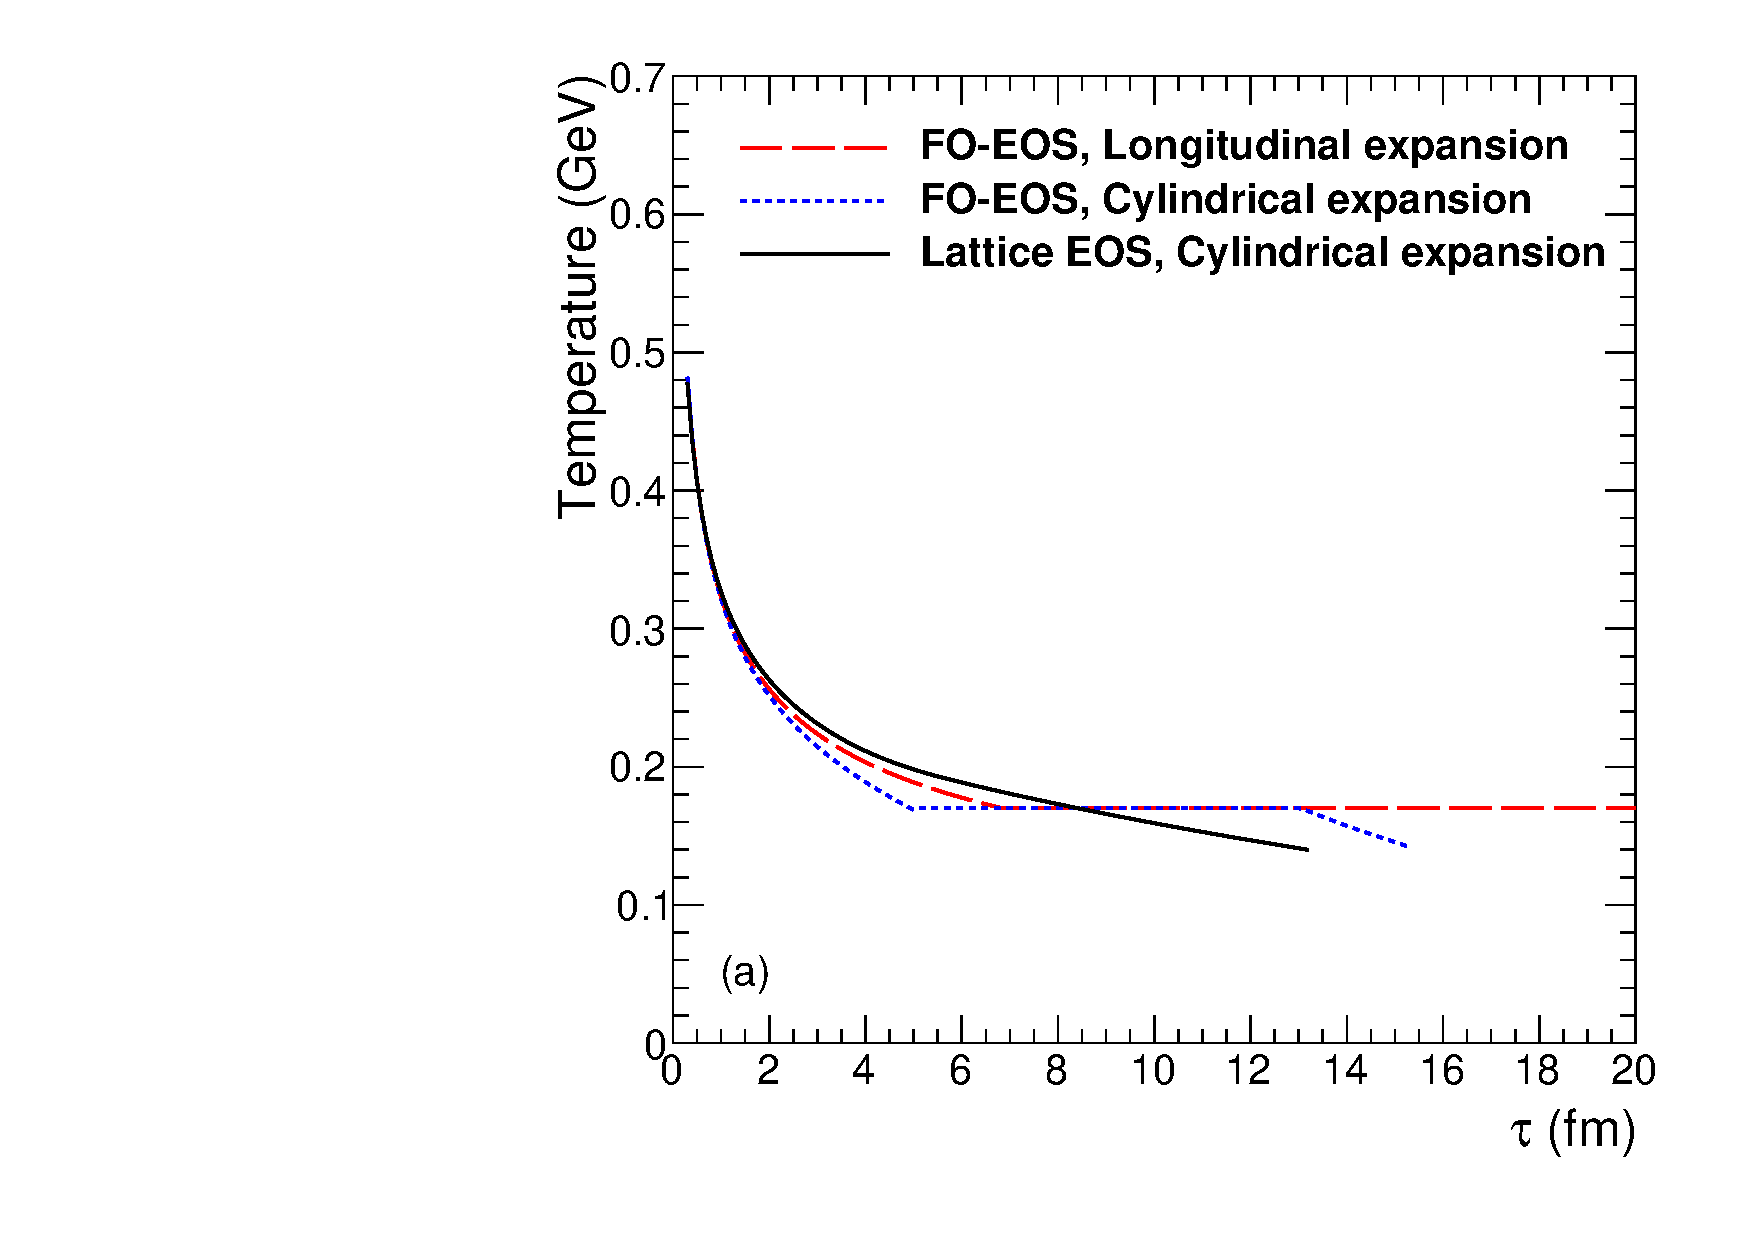
\includegraphics[width=0.49\textwidth]{Figures/Quarkonia_276TeV/Fig1a_TauVsTemp.pdf}
    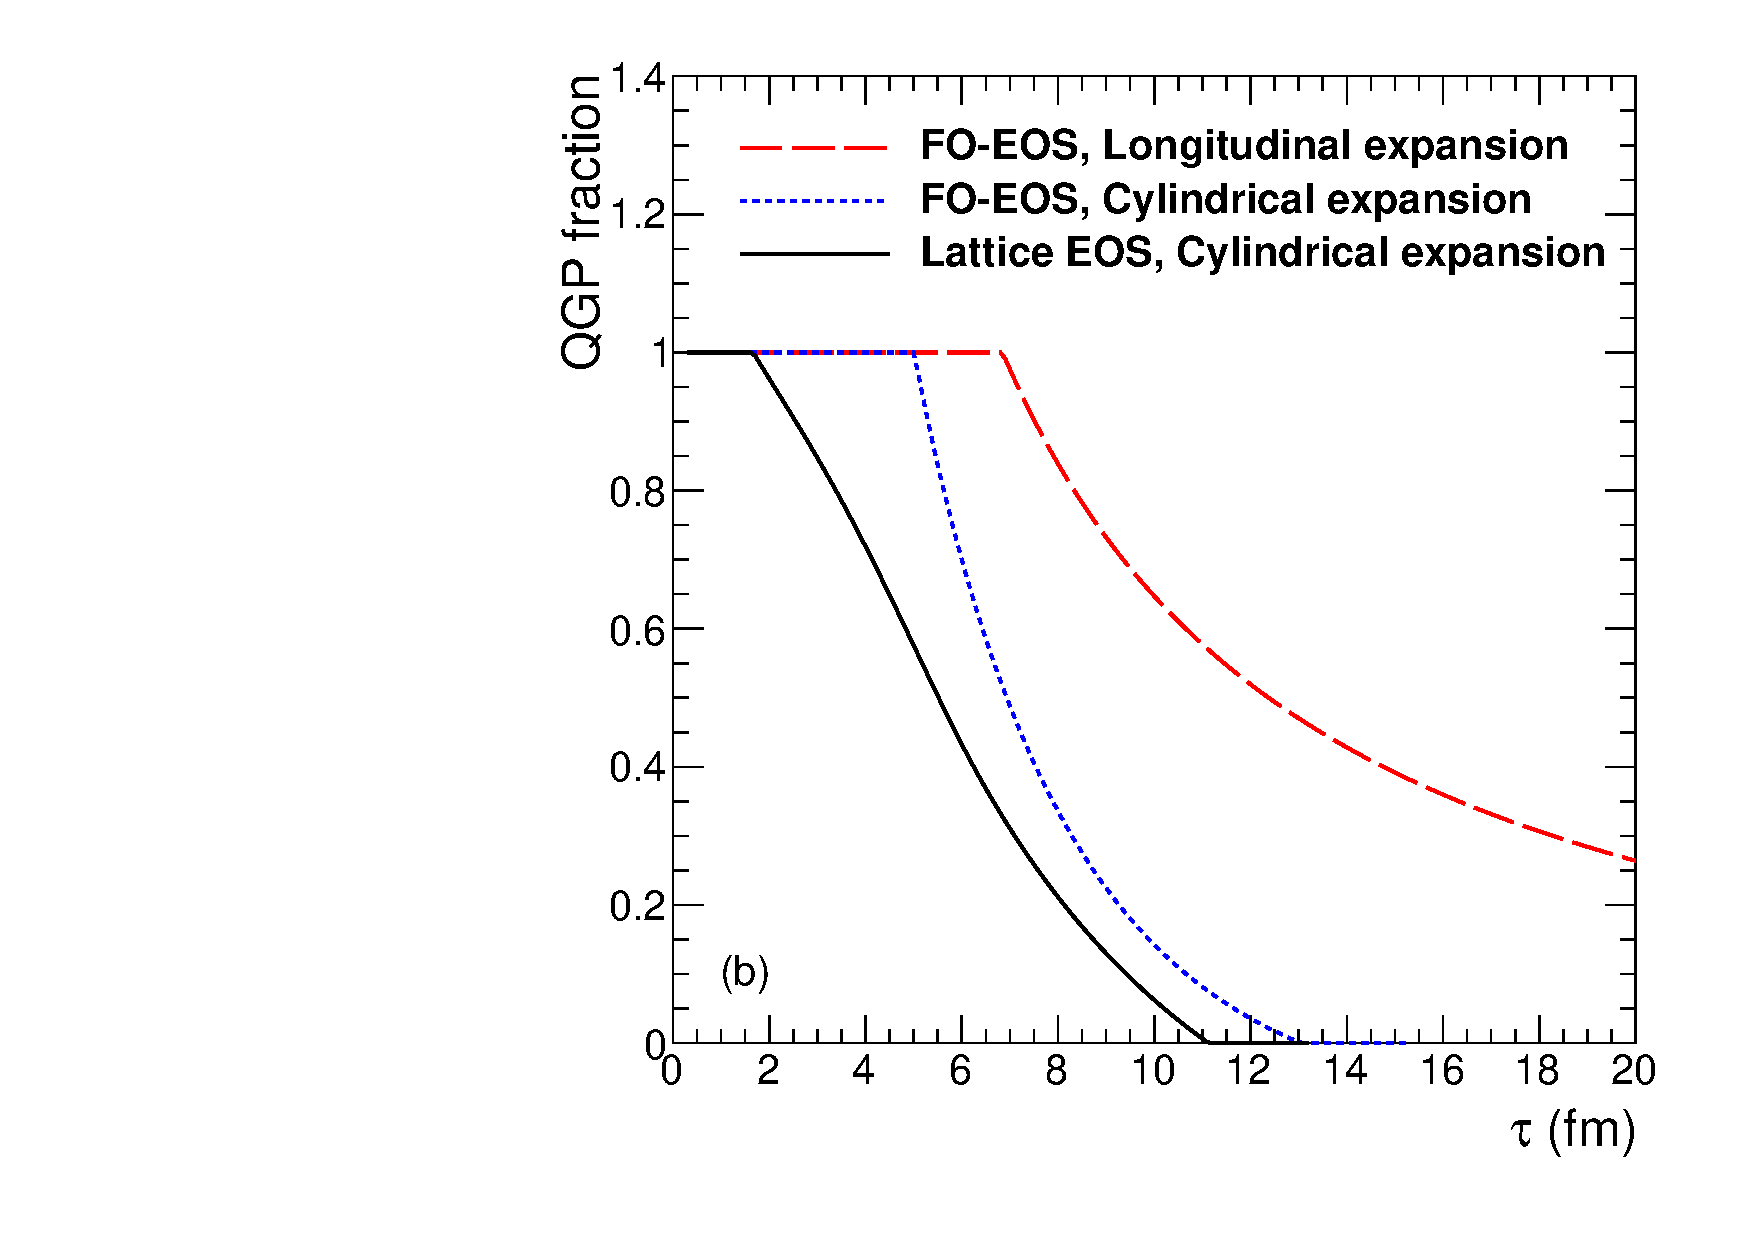
\includegraphics[width=0.49\textwidth]{Figures/Quarkonia_276TeV/Fig1b_TauVsFQGP.pdf}
    \caption{(Color online) (a) Temperature and (b) QGP fraction in the system as a function of proper 
      time $\tau$ in case of the most central (0-5$\%$) collisions for longitudinal and cylindrical expansions 
      using first order and lattice equation of state.}
    \label{fig:TauVsTemp}
  \end{figure}
  %%%%%%%%%%%%%%%%%%%%%%%%%%%%%%%%%%%%%%%%%%%%%%%%%%%%%%%%%%%%%%%%%%%%%%%%%%%%%%%%%%%%%%%%%%%%%%%%%
  \subsection{Dissociation Rate}
  In the color dipole approximation, the gluon dissociation cross section as function of gluon energy, $q^0$,
  in the quarkonium rest frame is~\cite{Bhanot:1979vb}
  \begin{equation}
    \sigma_{D}(q^{0}) = {8\pi \over 3} \, {16^2 \over 3^2} {a_0 \over m_q}  \frac{(q^0/\epsilon_0 - 1)^{3/2}} {(q^0/\epsilon_0)^5},
  \end{equation}
  where $\epsilon_0$ is the quarkonia binding energy and $m_q$ is the charm/bottom quark mass 
  and $a_0=1/\sqrt{m_q\epsilon_0}$.
  The values of $\epsilon_0$ are taken as 0.64 and 1.10 GeV for the ground states, $\Jpsi$ and $\Upsilon$(1S),
  respectively \cite{Karsch:1987pv}.
  For the first excited state of bottomonia, $\Upsilon$(2S), we use dissociation
  cross section from Ref.~\cite{Arleo:2001mp}.
  
  Figure \ref{fig:SigmaDQ0} shows the gluon dissociation cross sections of $\Jpsi$ and $\Upsilon$(1S)
  as a function of gluon energy. The dissociation cross section is zero when the gluon energy is less 
  than the binding energy of the quarkonia. It increases with gluon energy and reaches a maximum at 1.2 (1.5) GeV for 
  $\Jpsi~(\Upsilon(1{\rm S}))$. At higher gluon energies, the interaction probability decreases. The gluon energy $q^0$ 
  is related to the square of the center of mass energy $s$, of the quarkonium-gluon system by
  \begin{eqnarray}
    q^{0} = \frac{s-M_{Q}^{2}}{2\,M_{Q}}
  \end{eqnarray}  
  where $s=M_{Q}^{2} + 2  p_g \, \sqrt{M_{Q}^2 + p^2} - 2  p_g \, p \, {\rm cos\theta}$, and $M_{Q}$ and $p$ 
  are mass and momentum of quarkonium and $\theta$ is angle between the quarkonium and the gluon.
  We calculate the dissociation rate as a function of quarkonium momentum 
  by integrating the dissociation cross section over thermal gluon momentum 
  distribution $f_{g}(p_g)$,   
  \begin{eqnarray}
    \lambda_{D} \rho_{g}  & = & \langle \sigma v_{\rm rel} \rangle \,\rho_{g}  = \frac{g_g}{(2\pi)^{3}} \int d^{3}p_g \, f_{g}(p_g)  \, \sigma_{D}(s) v_{\rm rel}(s)  \nonumber \\ 
    & = & \frac{g_g}{(2\pi)^{3}} \int dp_g 2\pi p_g^{2} f_{g}(p_g) \int d\,{\rm cos\theta}\,\sigma_{D}(s)\,v_{\rm rel}(s),
  \end{eqnarray}
  where $\sigma_{D}(s) = \sigma_{D}(q^0(s))$.
  The relative velocity, $v_{\rm rel}$, between the quarkonium and the gluon is
  \begin{eqnarray}
    v_{\rm rel}  = {s- M_{Q}^{2} \over 2  p_g\sqrt{M_{Q}^2 + p^2}}.  
    \label{eq7}
  \end{eqnarray}
  The $\Jpsi$ gluon dissociation rates as a function of $T$ are shown in 
  Fig.~\ref{fig:DRateVsTempAndPt}(a) and as a function of $p_T$ in Fig.~\ref{fig:DRateVsTempAndPt}(b).
  The dissociation rate increases with temperature due to the increase in gluon density. 
  The dissociation rate is maximum when the quarkonium is at rest and decreases with $p_T$.

  
  \begin{figure}
    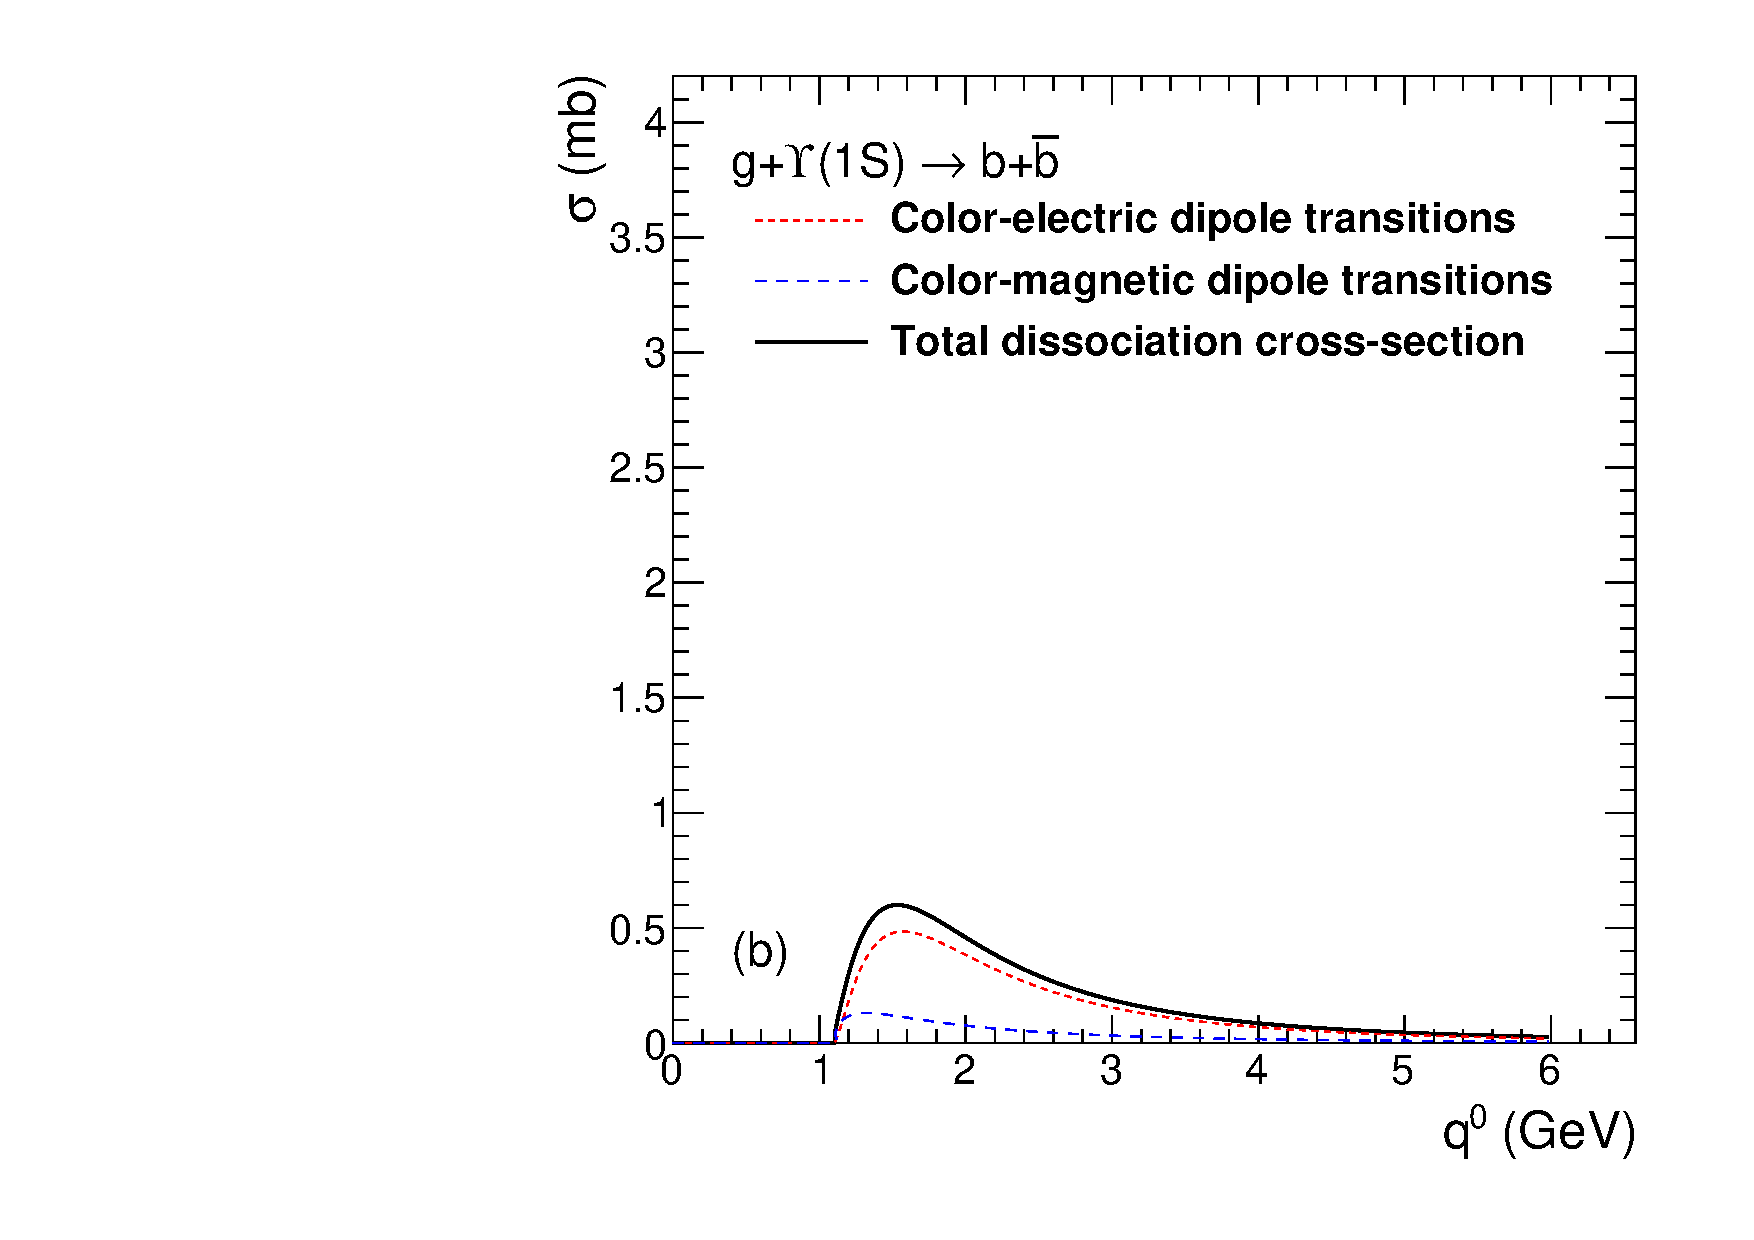
\includegraphics[width=0.60\textwidth]{Figures/Quarkonia_502TeV/Fig1b_Y1S_SigmaDq0.pdf}
    \caption{(Color online) Gluon dissociation cross section of quarkonia as a function of gluon energy ($q^{0}$) in
      quarkonia rest frame.}
    \label{fig:SigmaDQ0}
  \end{figure}
  


  \begin{figure}
    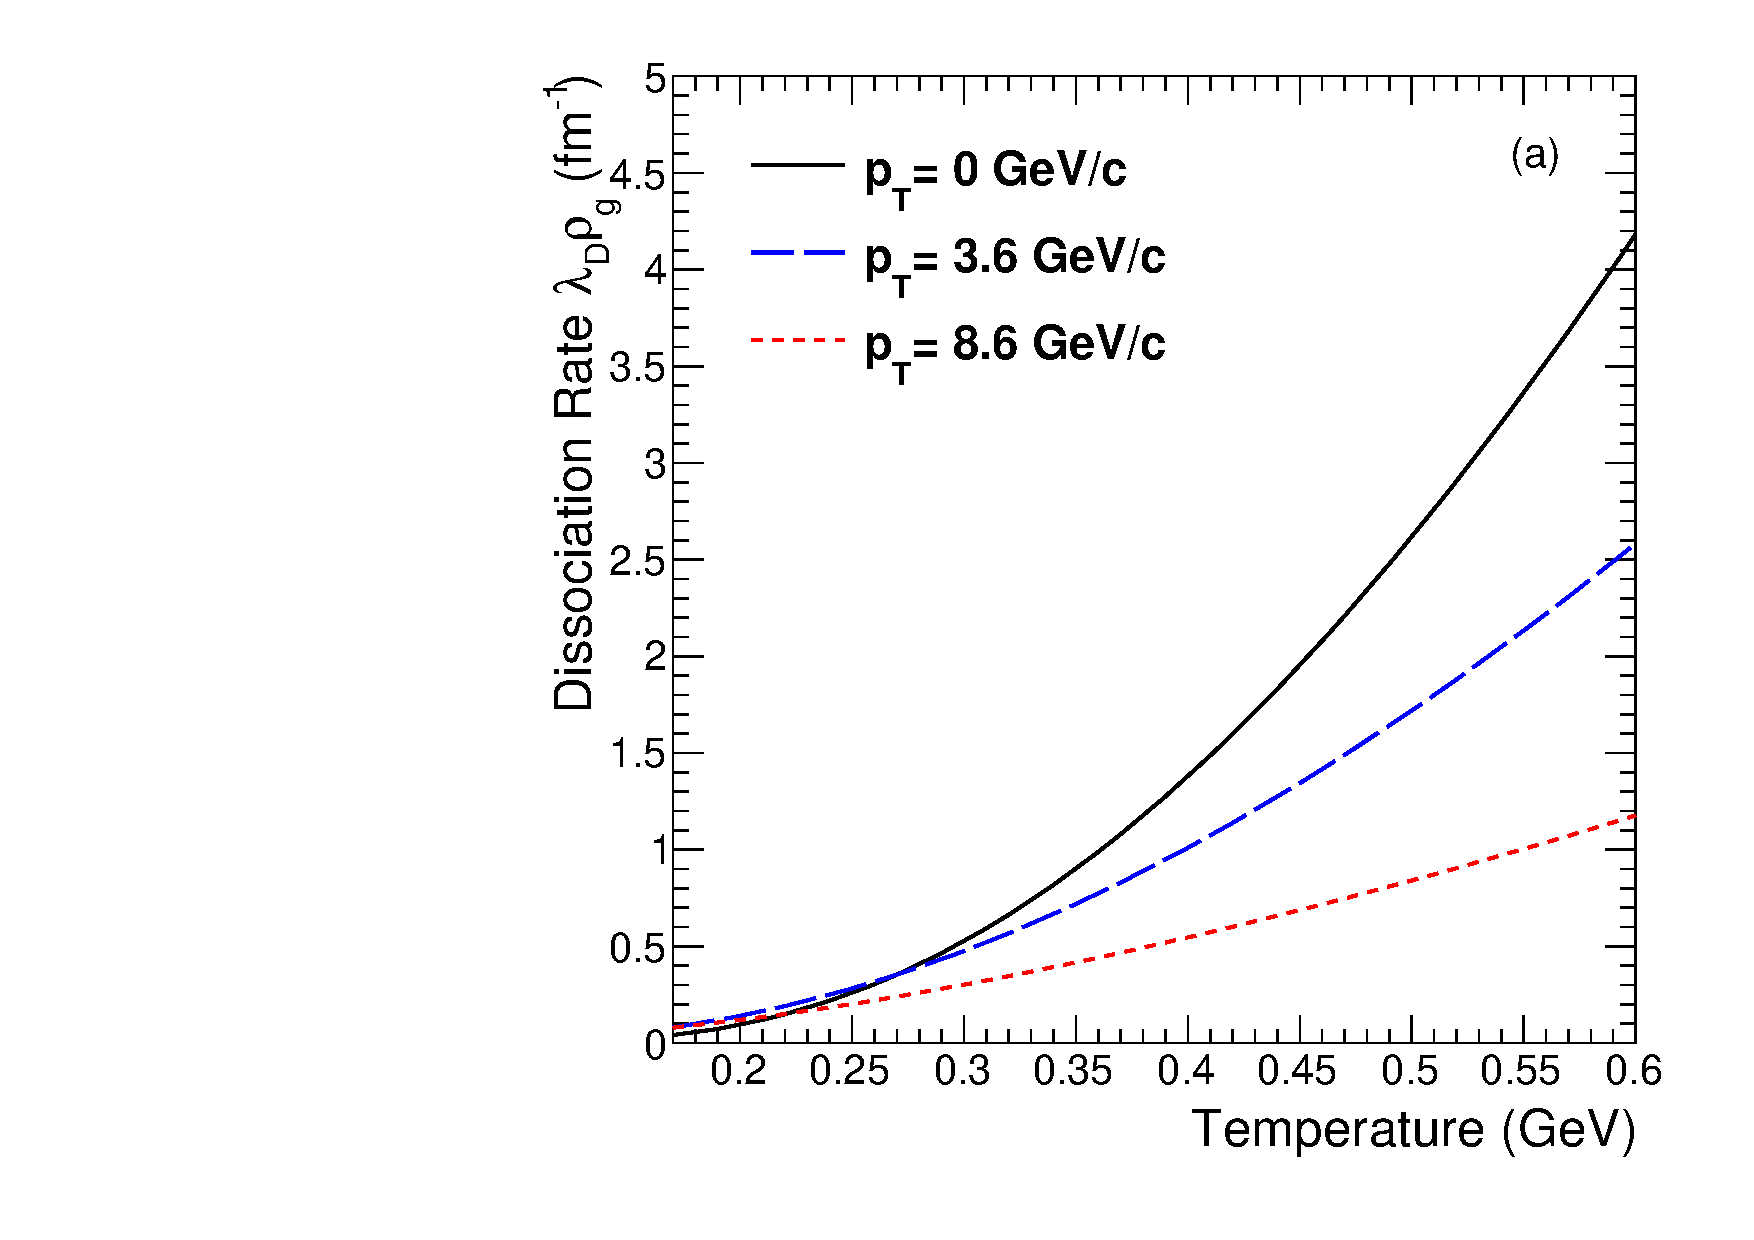
\includegraphics[width=0.49\textwidth]{Figures/Quarkonia_276TeV/Fig3a_DRateVsT.pdf}
    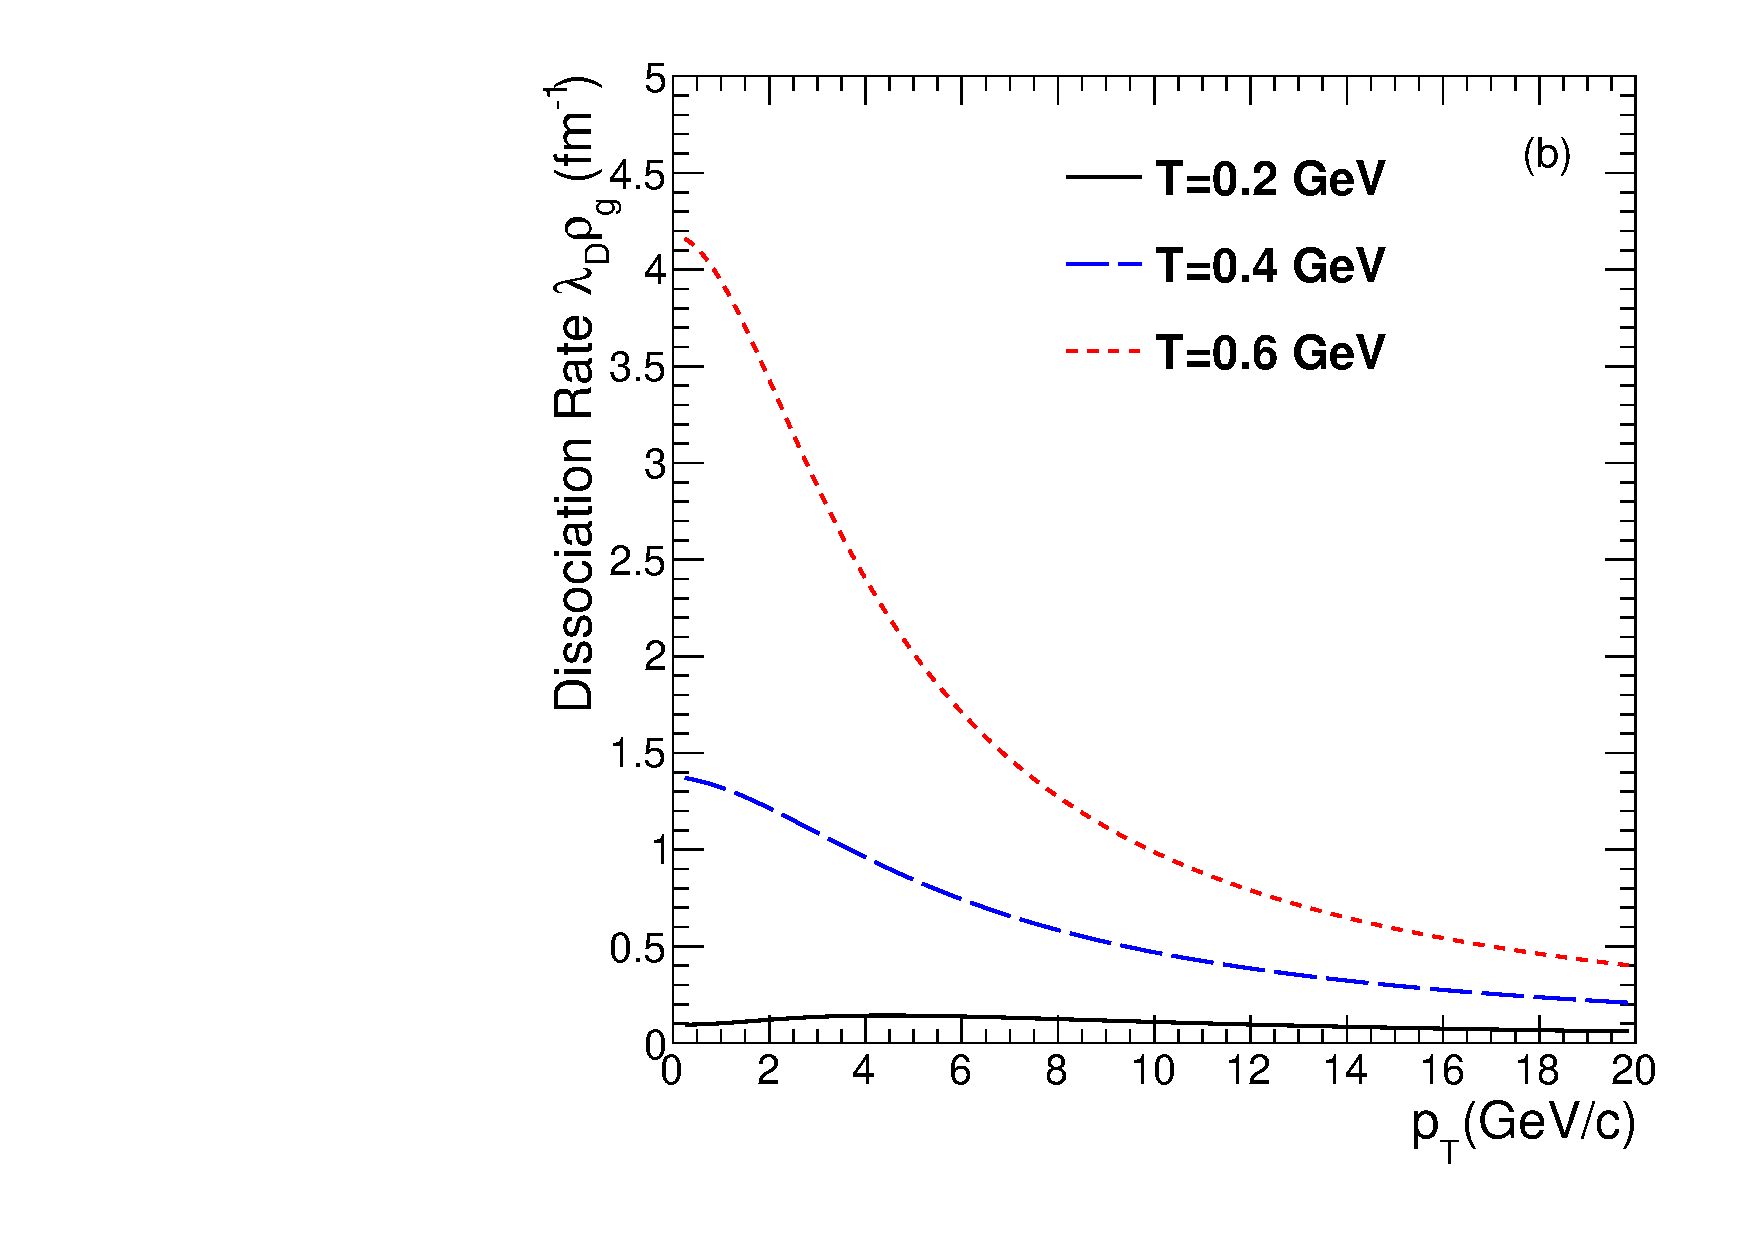
\includegraphics[width=0.49\textwidth]{Figures/Quarkonia_276TeV/Fig3b_DRateVsPt.pdf}
    \caption{(Color online) Gluon dissociation rate of $\Jpsi$ as a function of (a) temperature and  
      (b) transverse momentum.}
    \label{fig:DRateVsTempAndPt}
  \end{figure}
  \subsection{Formation Rate}
  We can calculate the formation cross section from the dissociation cross section using detailed balance~\cite{Thews:2000rj,Thews:2005vj},
  \begin{equation}
    \sigma_{F} = \frac{48}{36}\,\sigma_{D}(q^0)\frac{(s-M_{Q}^2)^{2}}{s(s-4m_q^{2})}.
  \end{equation}
  The formation rate of quarkonium with momentum {\bf p} can be written as
  \begin{equation}
    \frac{d\lambda_{F}}{d{\rm\bf p}} = \int \,d^{3}p_1 \,d^{3}p_2 \,\sigma_{F}(s)\, v_{\rm rel}(s)\,f_{q}(p_1)\, f_{\bar{q}} (p_2)\,\delta({\rm\bf p}-( {\rm\bf p_1} + {\rm\bf p_2} )).
  \end{equation}
  Here $f_{q/\bar{q}}(p)$ are taken as thermal distribution function of  $q/\bar{q}$ which are 
  normalized to one, $\int f_{q}(p) d^{3}p  = 1 $ and $v_{\rm rel}$ is relative velocity of the
  $q\bar{q}$ quark pair,
  \begin{eqnarray}
    v_{\rm rel} &=& {\sqrt{(p_{1}.p_{2})^{2} - m_q^{4} } \over E_{1} \, E_{2}}. %\nonumber \\
  \end{eqnarray}
  Here $p_1 = (E_1,{\bf p_{1}})$ and $p_{2} = (E_{2},{\bf p_{2}})$ are the four momenta of the heavy quark and 
  antiquark respectively.
  Figure \ref{fig:ForRateVsTempAndPt} (a) shows the variation of the formation rate as a function 
  of $T$ and Fig.~\ref{fig:ForRateVsTempAndPt} (b) shows as a function of $\Jpsi$ $p_T$.
  The $\Jpsi$ generated from recombination of uncorrelated heavy quark pairs will have 
  softer $p_{T}$ distributions than those of $\Jpsi$'s coming from the initial hard scatterings.
  Thus the effect of recombination will be important only at low $p_T$.
  
  \begin{figure}
    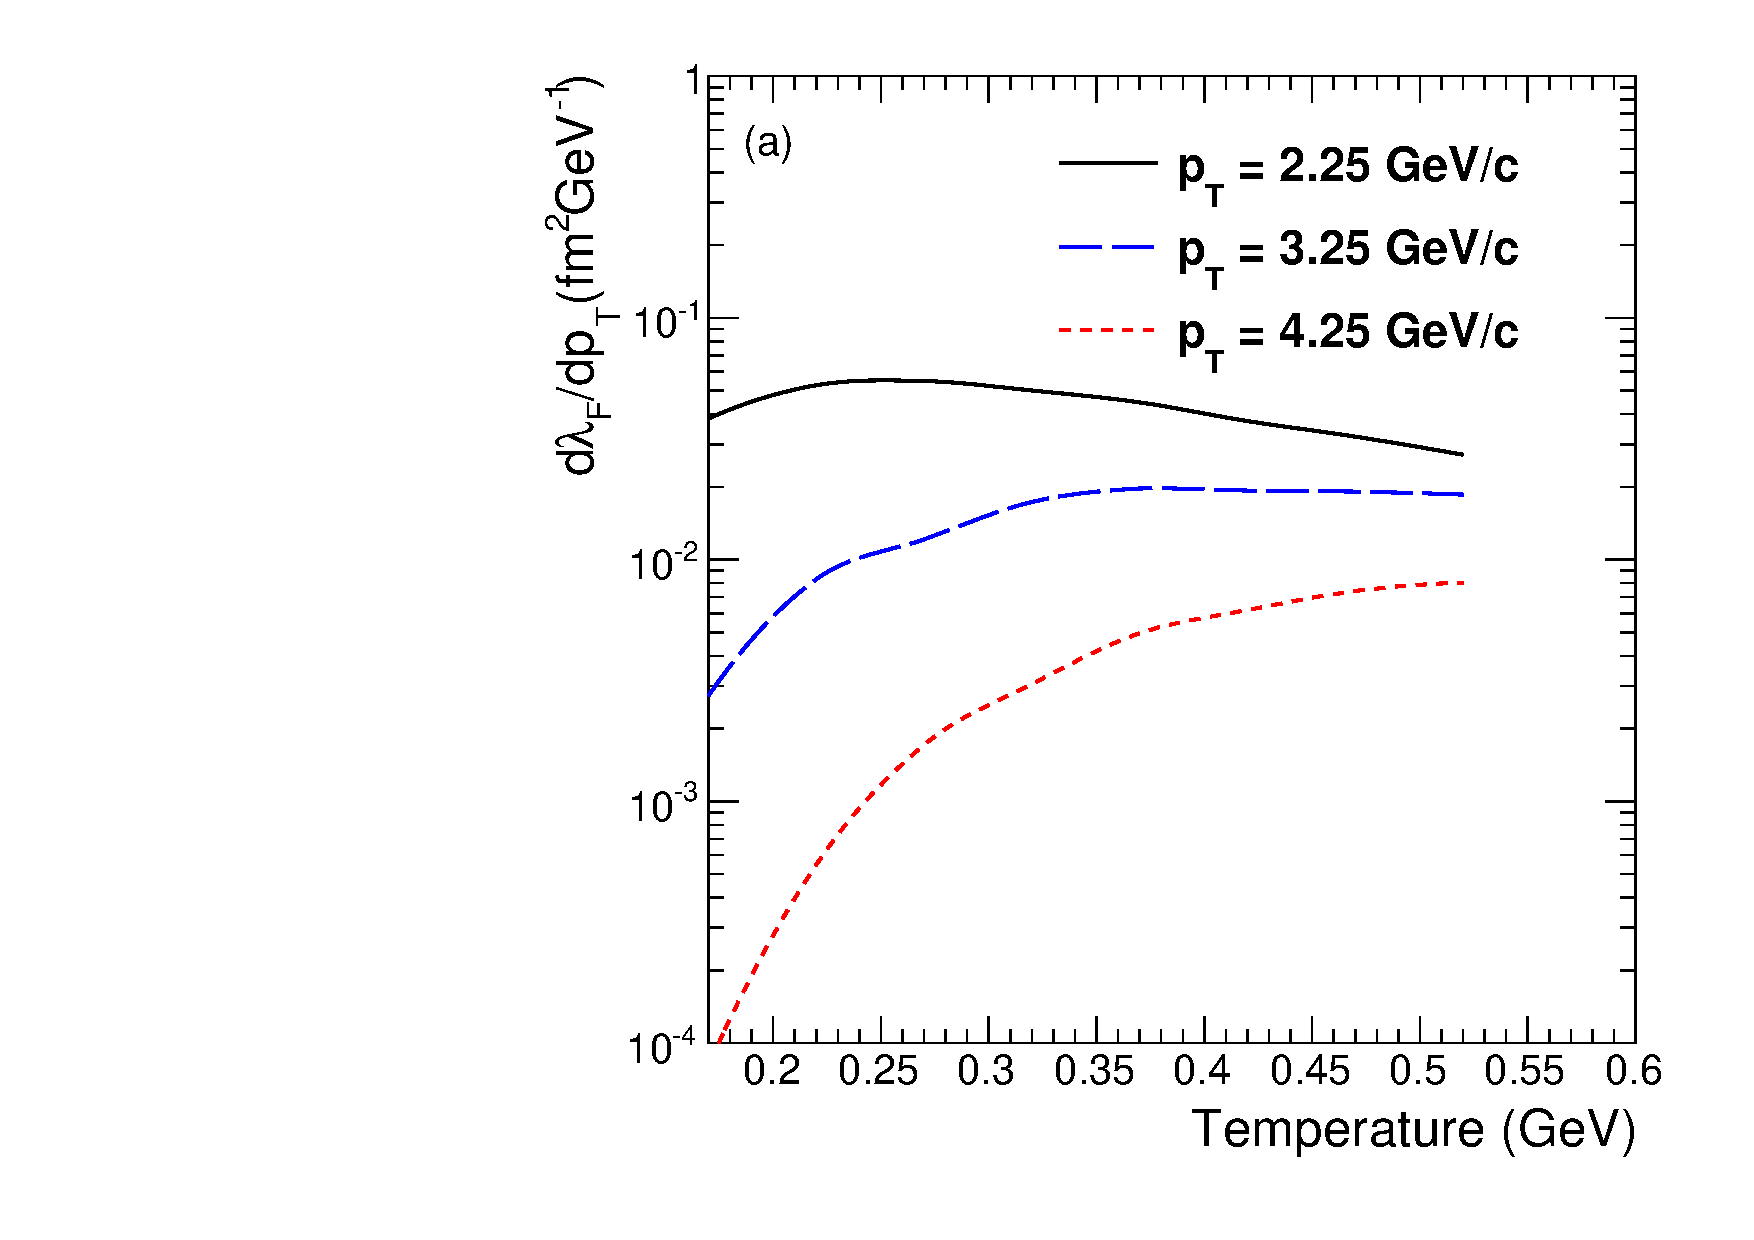
\includegraphics[width=0.49\textwidth]{Figures/Quarkonia_276TeV/Fig4a_FRateVsT.pdf}
    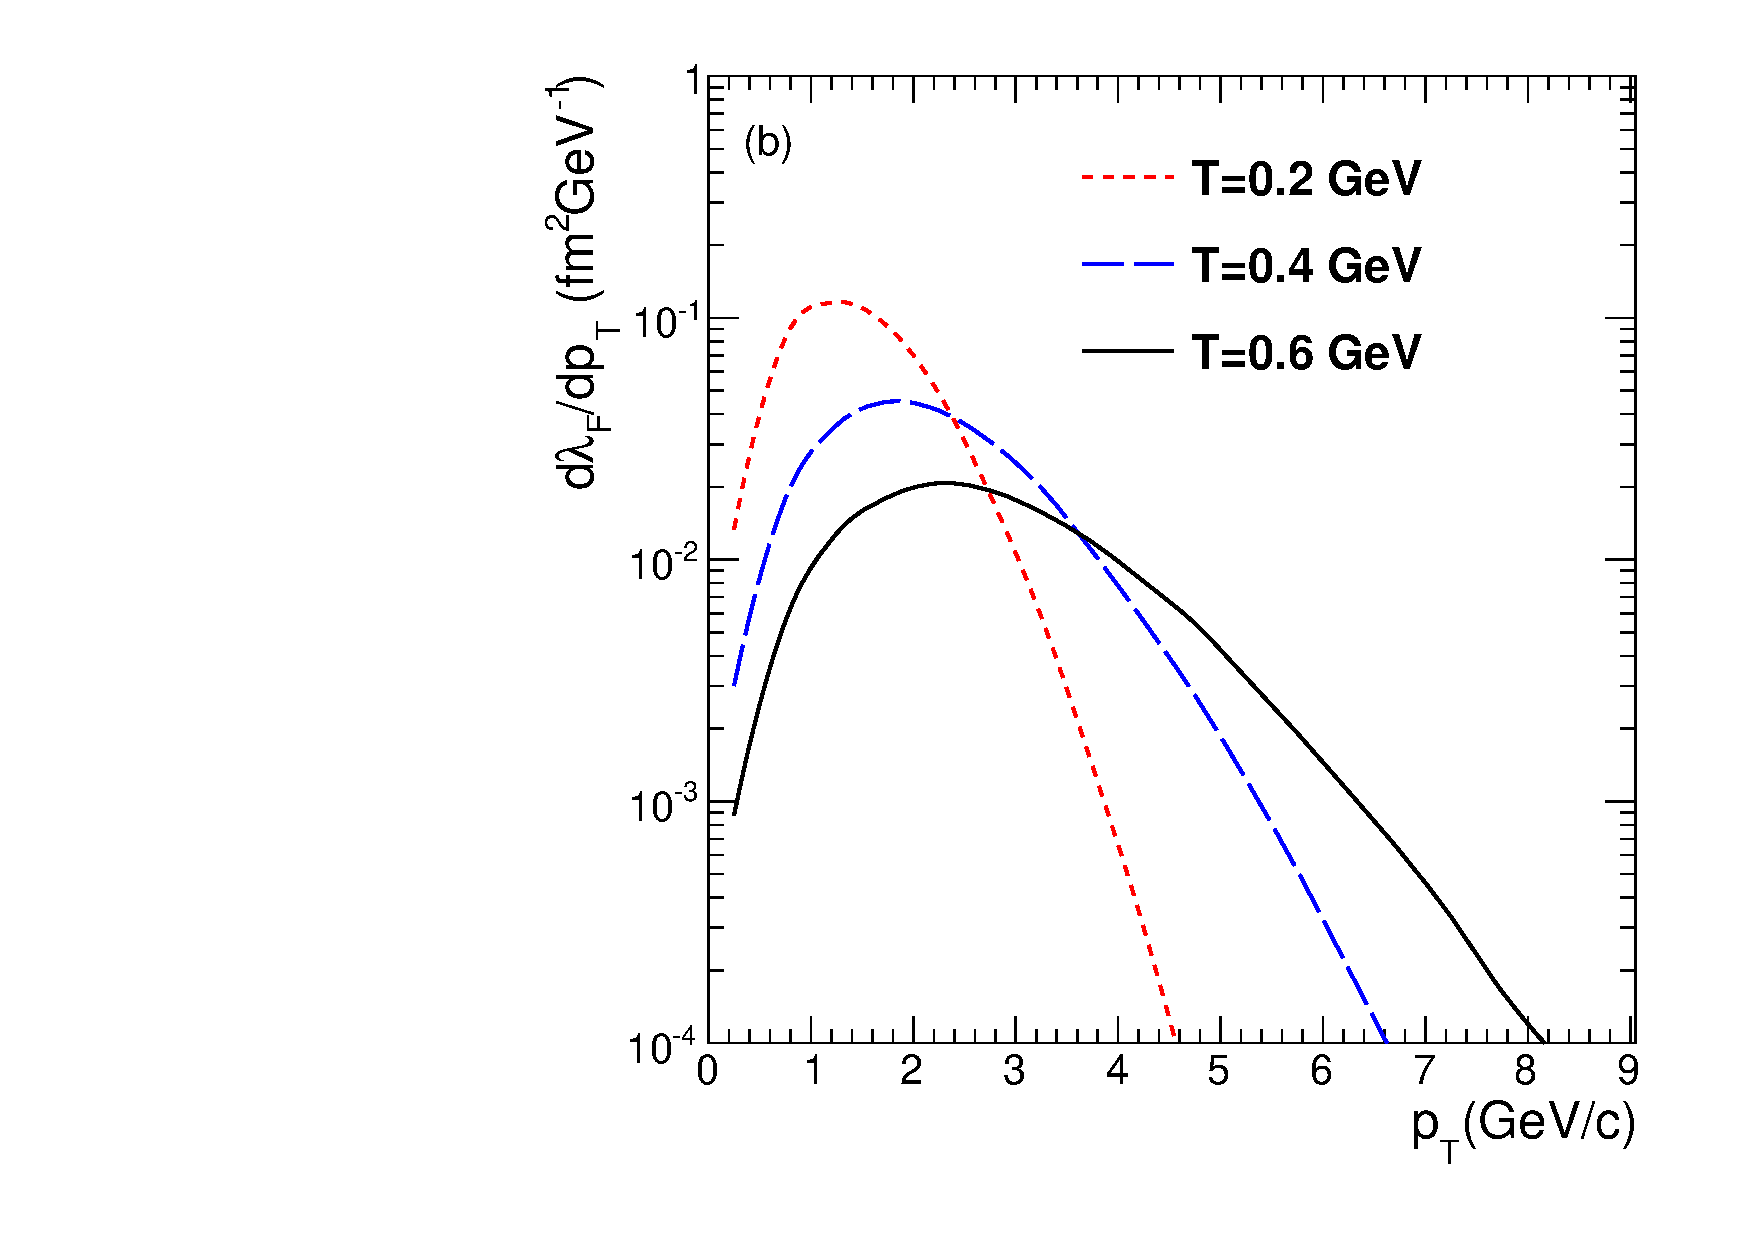
\includegraphics[width=0.49\textwidth]{Figures/Quarkonia_276TeV/Fig4b_FRateVsPt.pdf}
    \caption{(Color online) Formation rate of  $\Jpsi$ as a function of (a) temperature and 
      (b) transverse momentum.}
    \label{fig:ForRateVsTempAndPt}
  \end{figure}
  
  
  \begin{figure}
    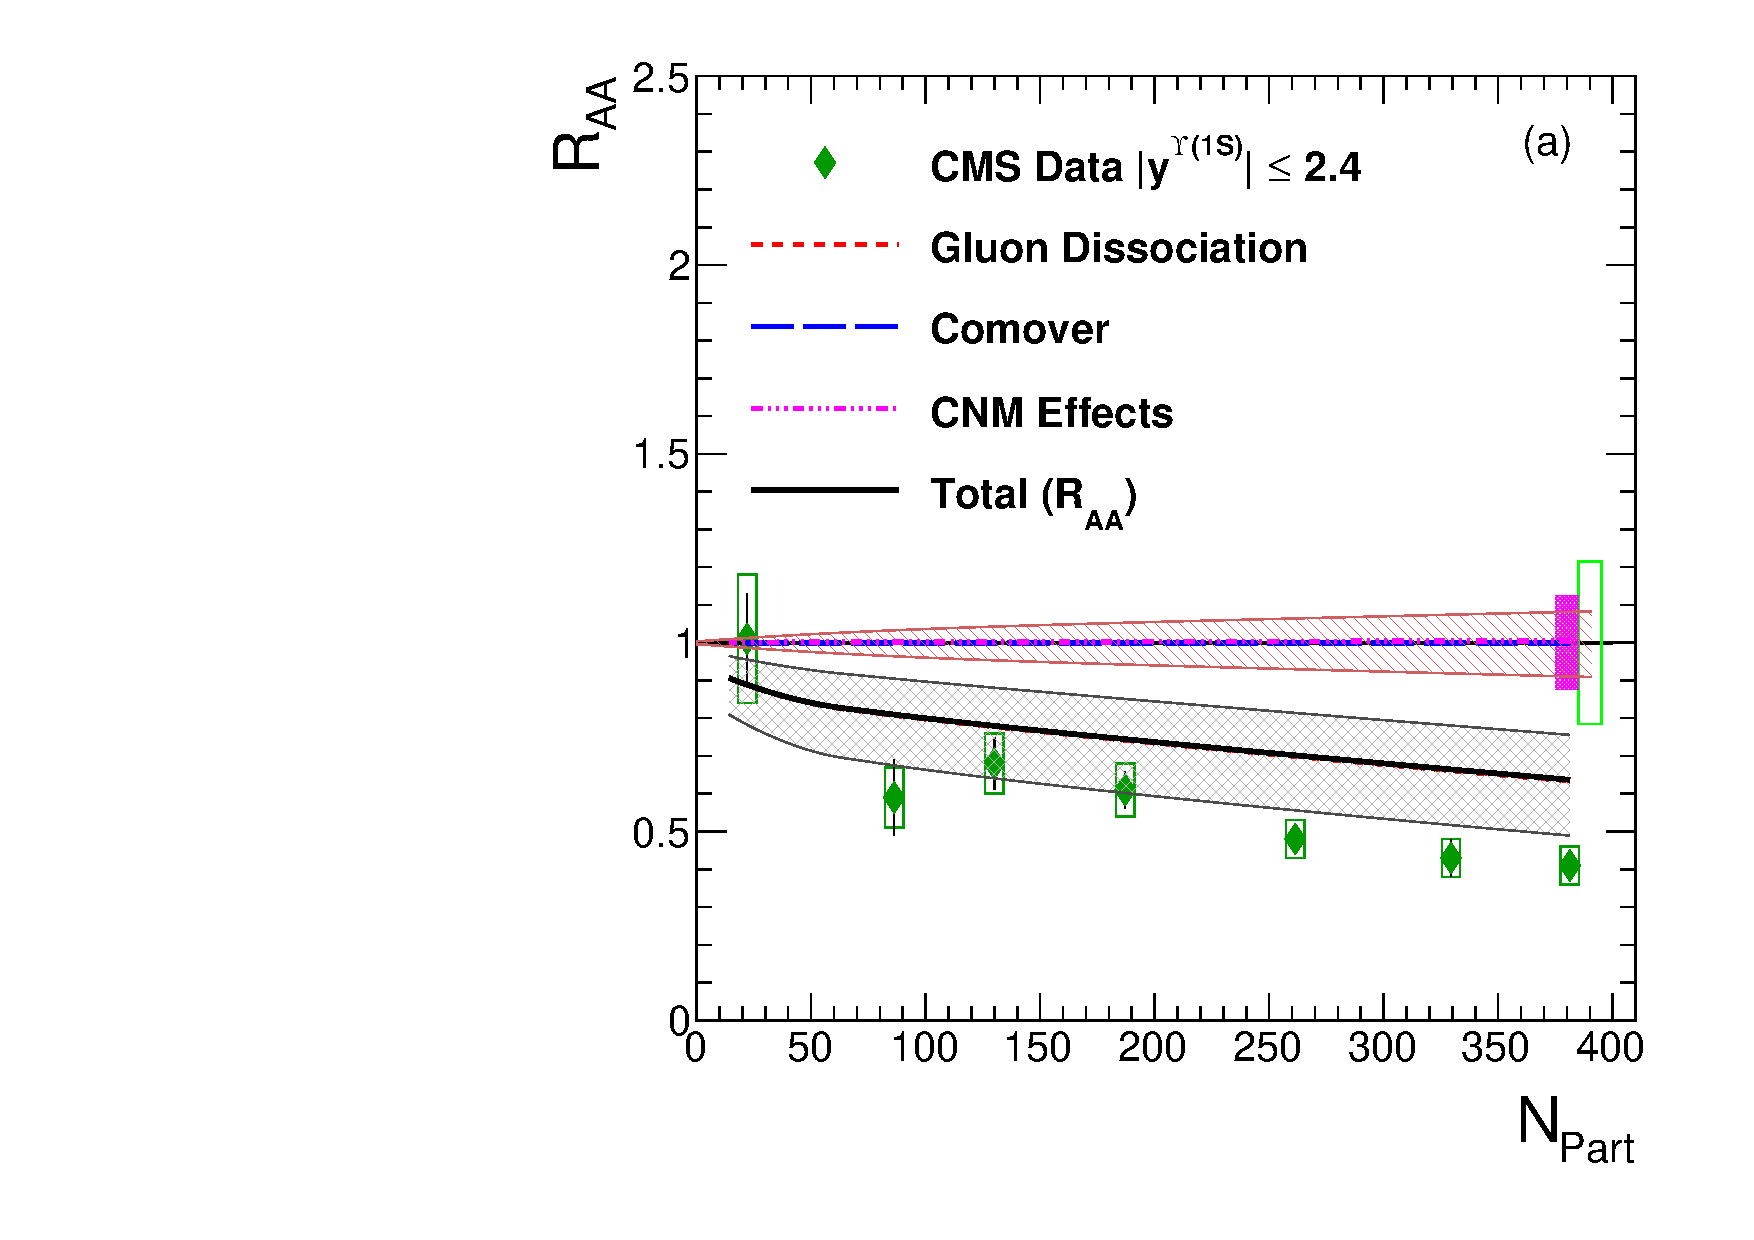
\includegraphics[width=0.49\textwidth]{Figures/Quarkonia_276TeV/Fig8a_CMS_Y1SRAANPart.pdf}
    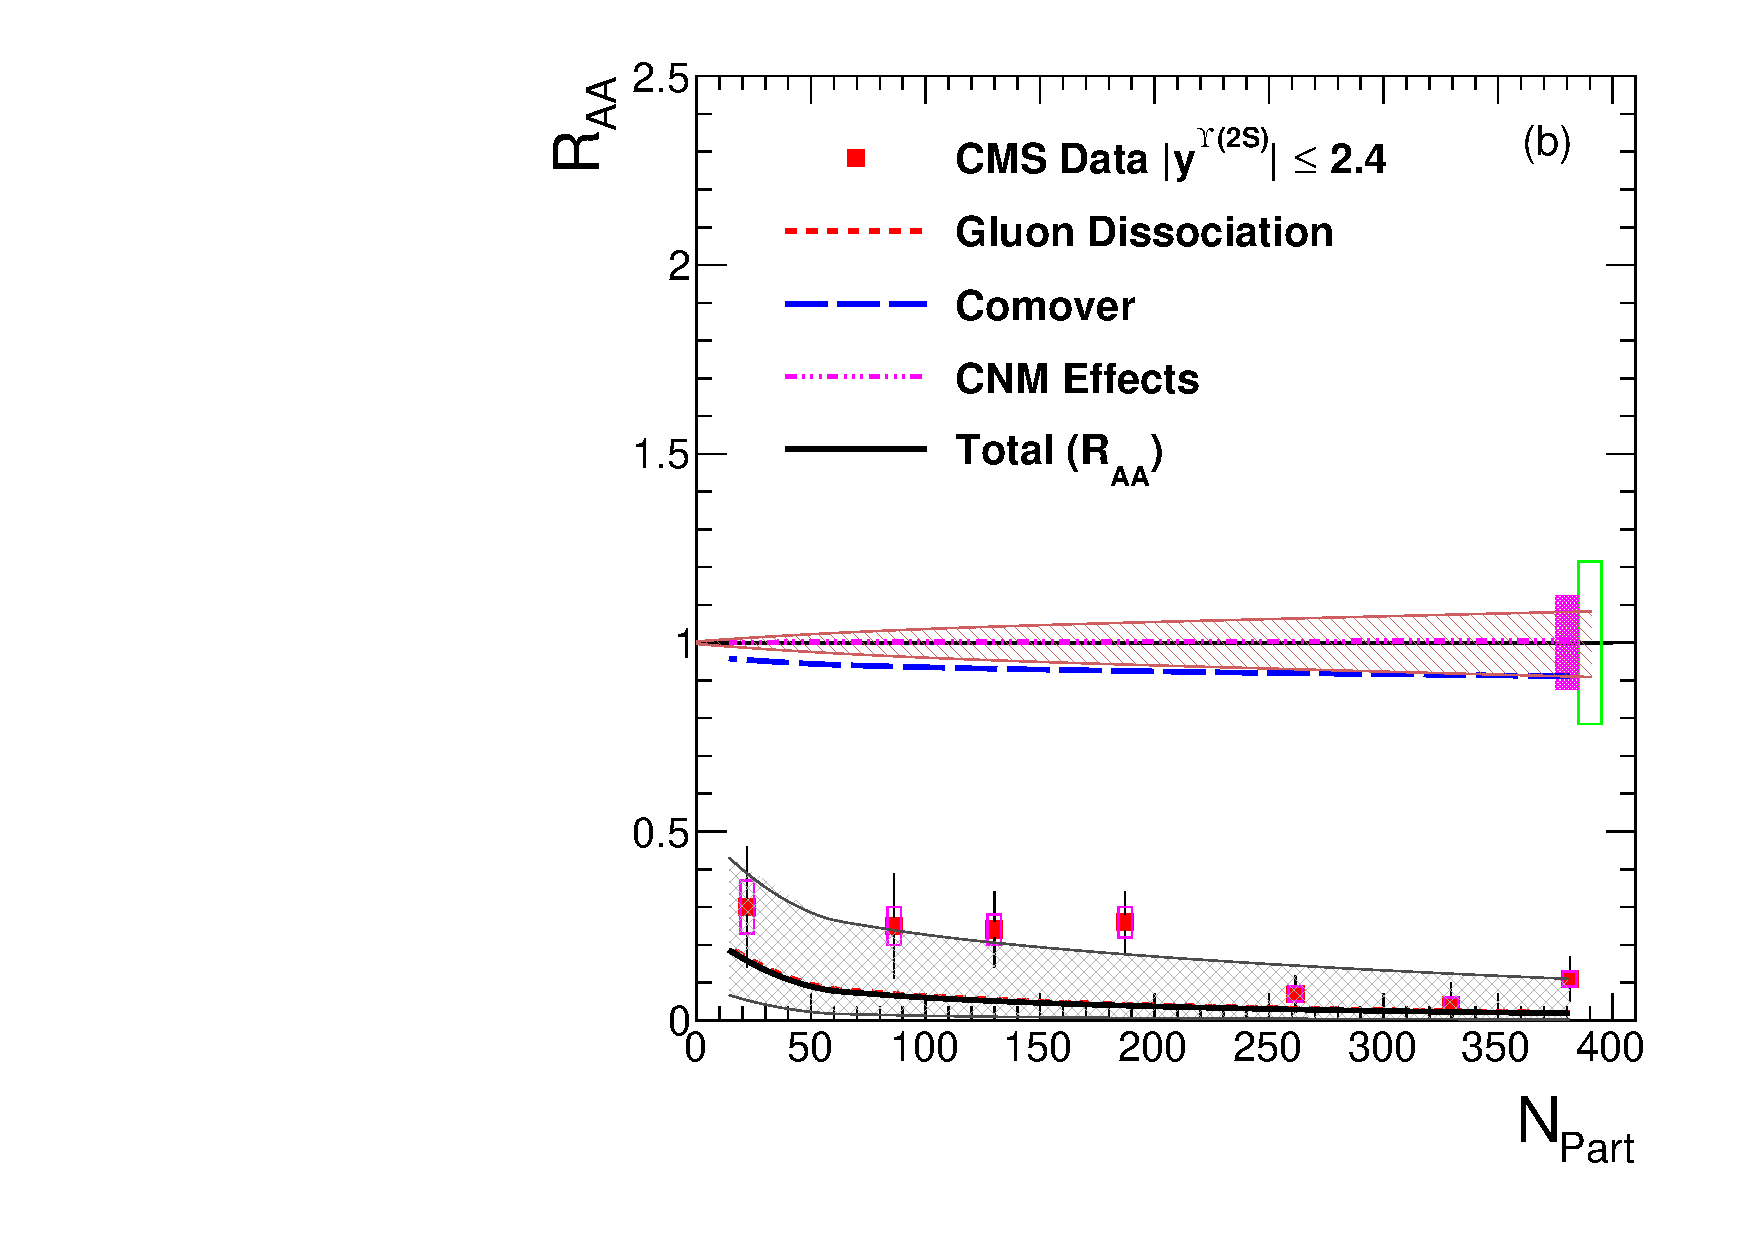
\includegraphics[width=0.49\textwidth]{Figures/Quarkonia_276TeV/Fig8b_CMS_Y2SRAANPart.pdf}
    \caption{(Color online) Calculated nuclear modification factor ($R_{AA}$) compared with CMS 
      (a) $\Upsilon$(1S) and (b) $\Upsilon$(2S) measurements. Regeneration is assumed to be negligible. }
    \label{fig:UpsilonRaa}
  \end{figure}
  \begin{figure}
    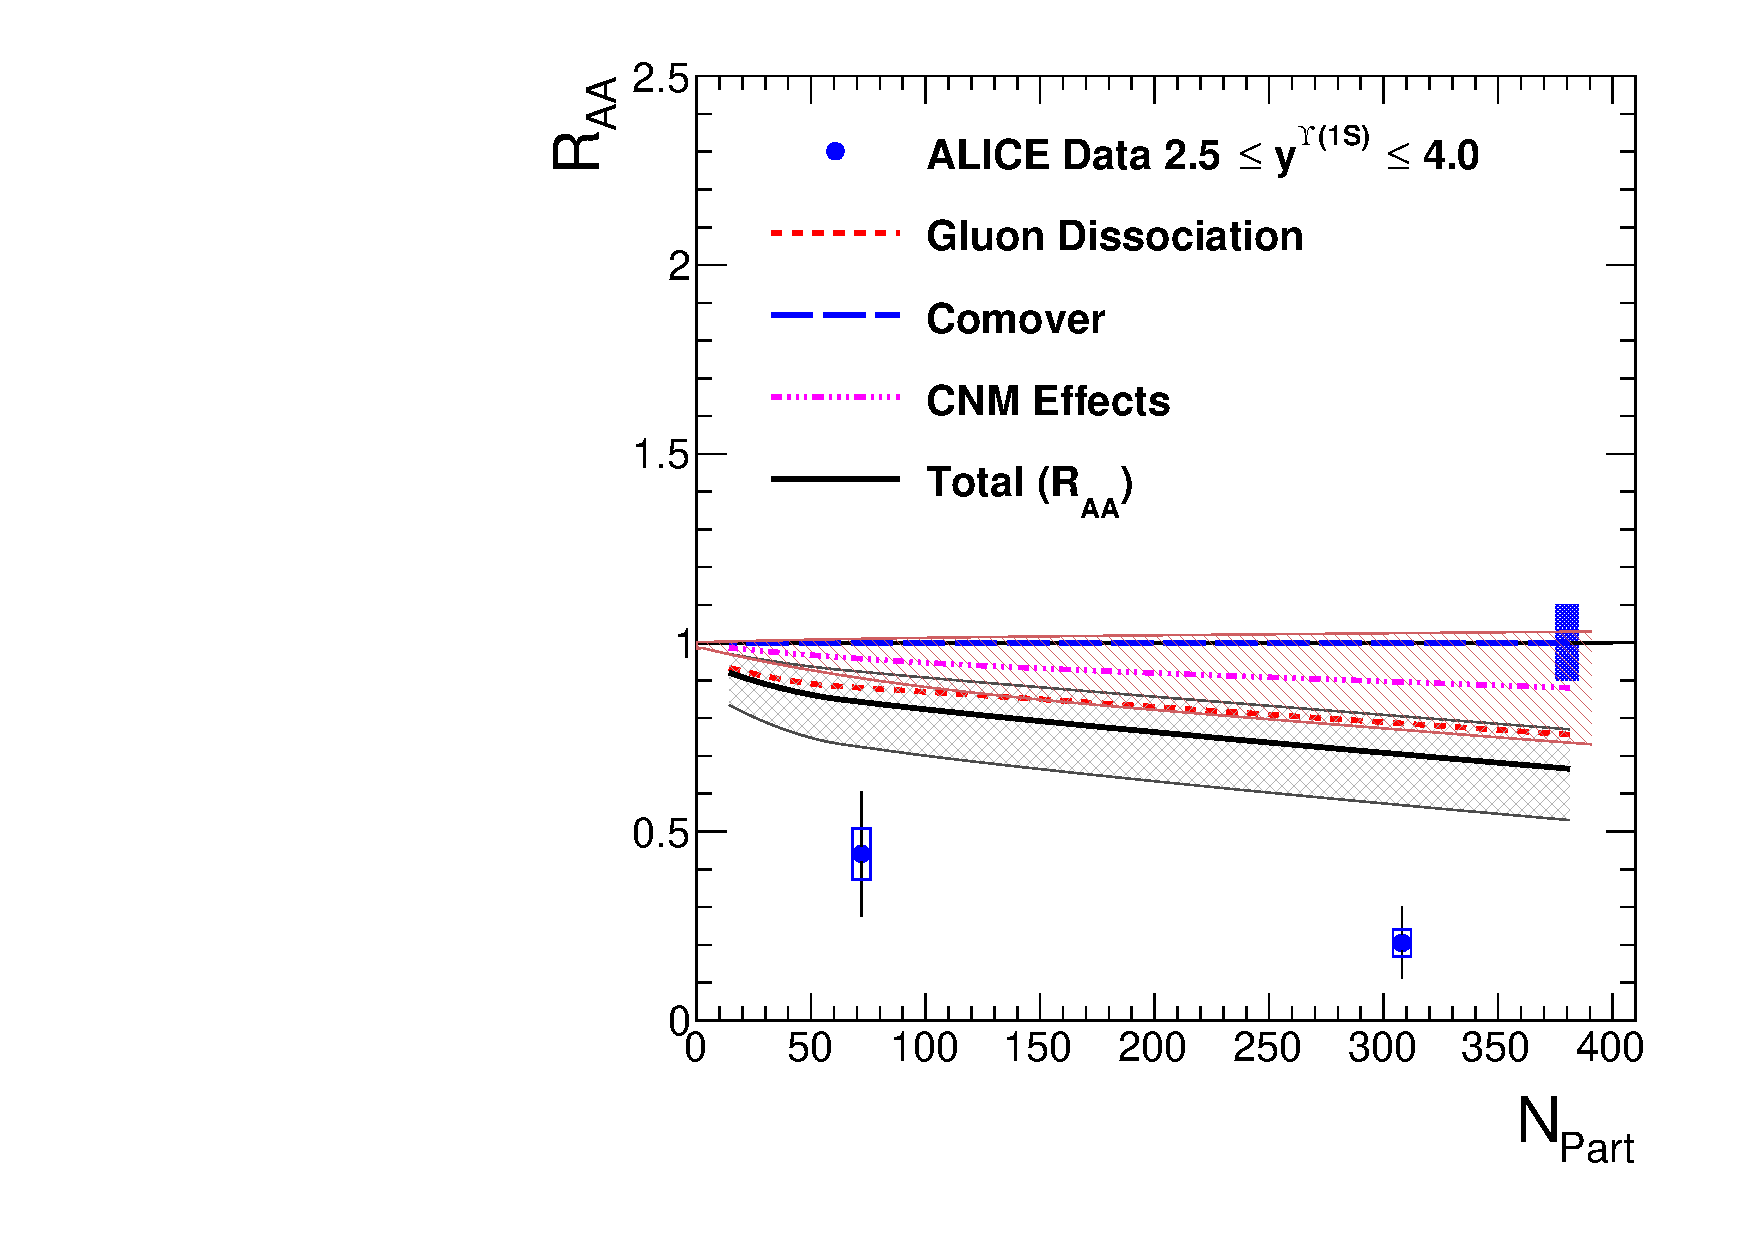
\includegraphics[width=0.49\textwidth]{Figures/Quarkonia_276TeV/Fig9_ALICE_Y1SRAANPart.pdf}
    \caption{(Color online) Calculated nuclear modification factor ($R_{AA}$) compared with 
      ALICE $\Upsilon$(1S) measurement in forward rapidity.}
    \label{fig:ALICERaaY}
  \end{figure}




Figure~\ref{fig:UpsilonRaa} (a) demonstrates the contributions from different processes to the 
centrality dependence of the $\Upsilon$(1S) nuclear modification factor, along with the midrapidity 
data from CMS~\cite{Chatrchyan:2012lxa}. The calculations underestimate the suppression but reproduce 
the shape of centrality dependence. This may be due to the feed down effects from the excited states. 
Figure~\ref{fig:UpsilonRaa} (b) shows the same for the $\Upsilon$(2S) nuclear modification factor
along with the CMS measurements at midrapidity. The excited $\Upsilon$(2S) states 
are highly suppressed. The effect of regeneration, not shown, is negligible 
for the $\Upsilon$ states. 
{\color{black} Figure~\ref{fig:ALICERaaY} shows the forward rapidity 
  ALICE measurement of the $\Upsilon$(1S) nuclear modification factor \cite{Abelev:2014nua}
  along with our calculations. The suppression due to thermal gluon dissociation is smaller 
  than the measured suppression which may be due to the effect of feed down from the $\Upsilon$(2S)
  and higher states.} 
{\color{black} However the measurement is consistent with the suppression of $\Upsilon$(2S) and  
  $\Upsilon$(3S) contribution, along with suppression of the $\Upsilon$(1S) by gluon 
  dissociation.
}


%%%%%%%%%%%%%%%%%%%%%%%%%%%%%%%%%%%%%%%%%%%%%%%%%%%%%%%% 5.02 TeV %%%%%%%%%%%%%%%%%%%%%%%%%%%%%%%%%%%%%%%%%
\begin{figure}
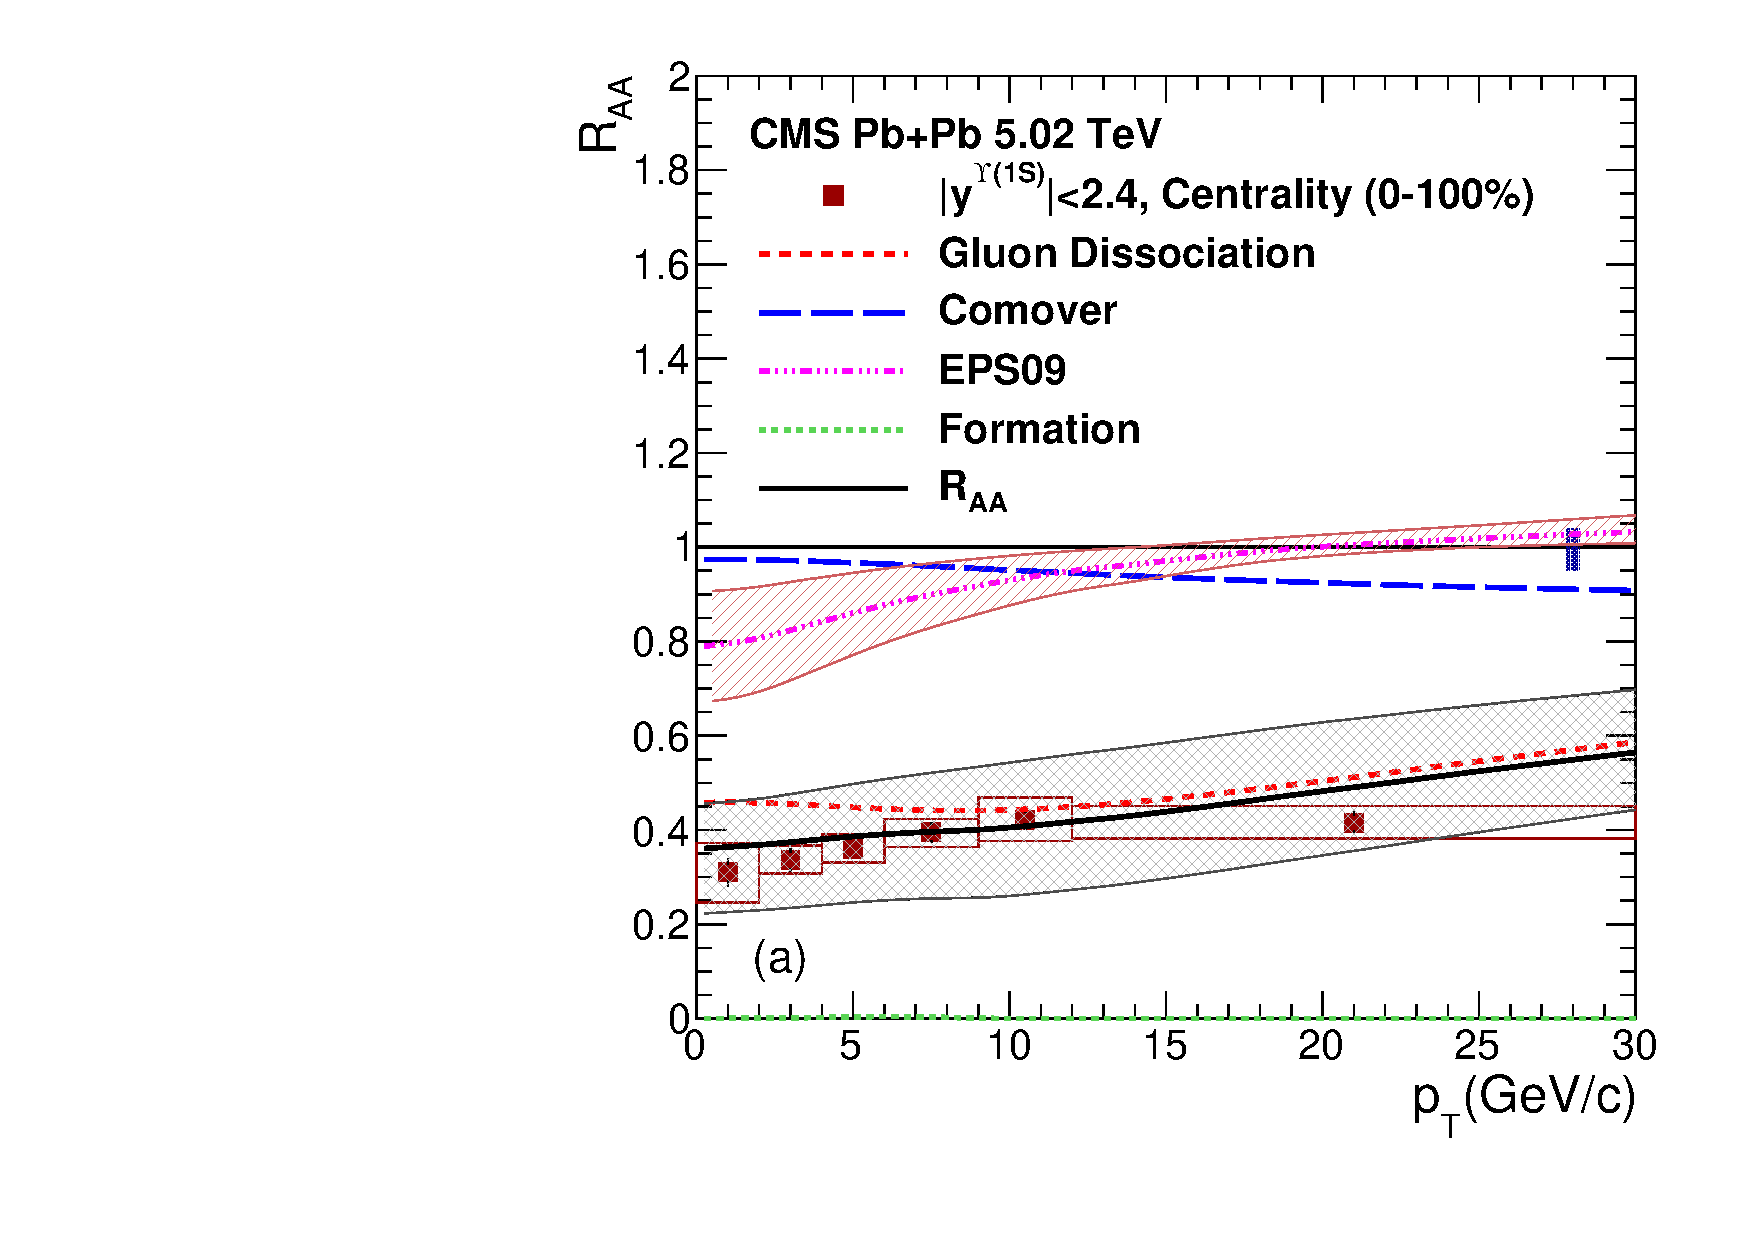
\includegraphics[width=0.49\textwidth]{Figures/Quarkonia_502TeV/Fig7a_Y1S_CMS_RAAPt_Shade.pdf}
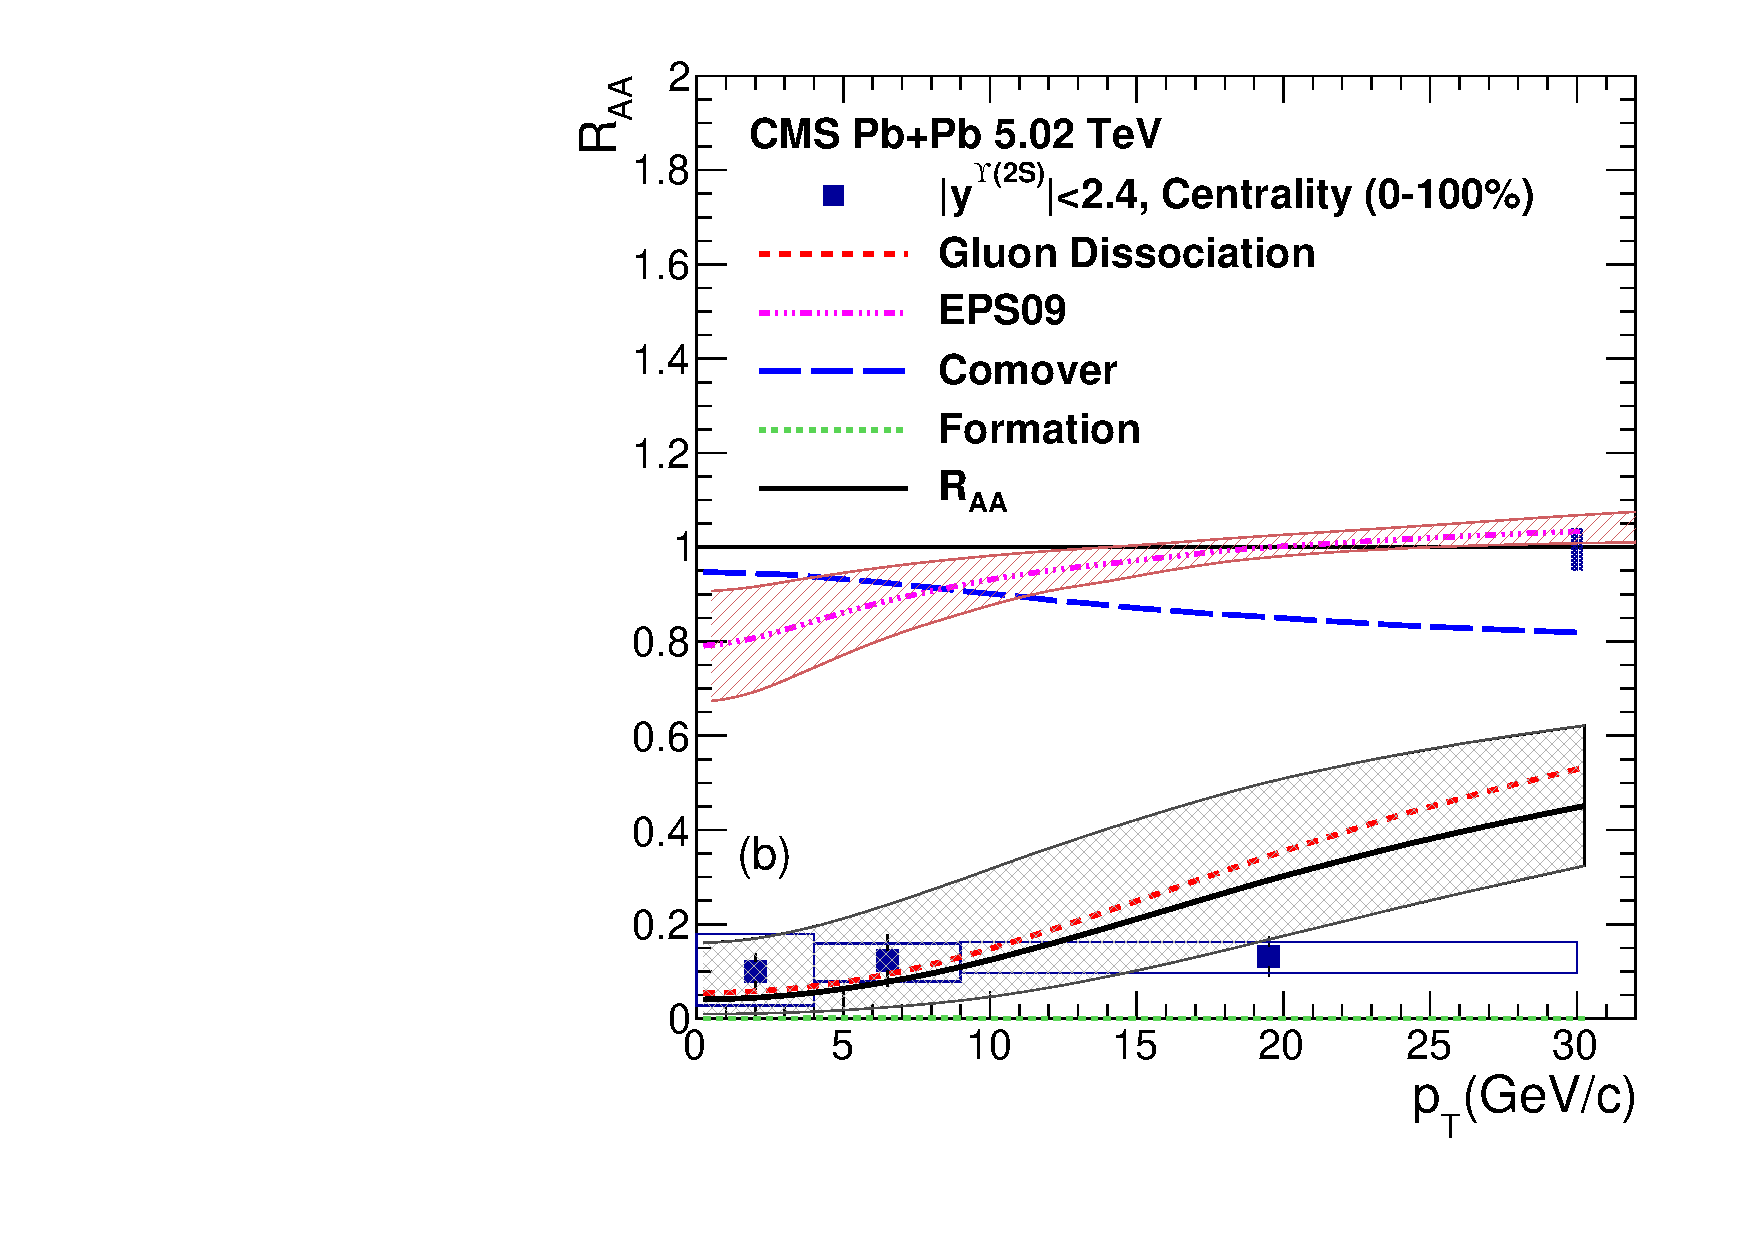
\includegraphics[width=0.49\textwidth]{Figures/Quarkonia_502TeV/Fig7b_Y2S_CMS_RAAPt_Shade.pdf}
\caption{(Color online) Calculated nuclear modification factor ($R_{AA}$) of (a) $\Upsilon$(1S) and 
  (b) $\Upsilon$(2S) as a function of $p_{T}$ 
  compared with CMS measurements~\cite{Sirunyan:2018nsz}.
The global uncertainty in $R_{AA}$ is shown as a band around the line at 1.
}
\label{fig:UpsilonRaaPtCMS}
\end{figure}



\begin{figure}
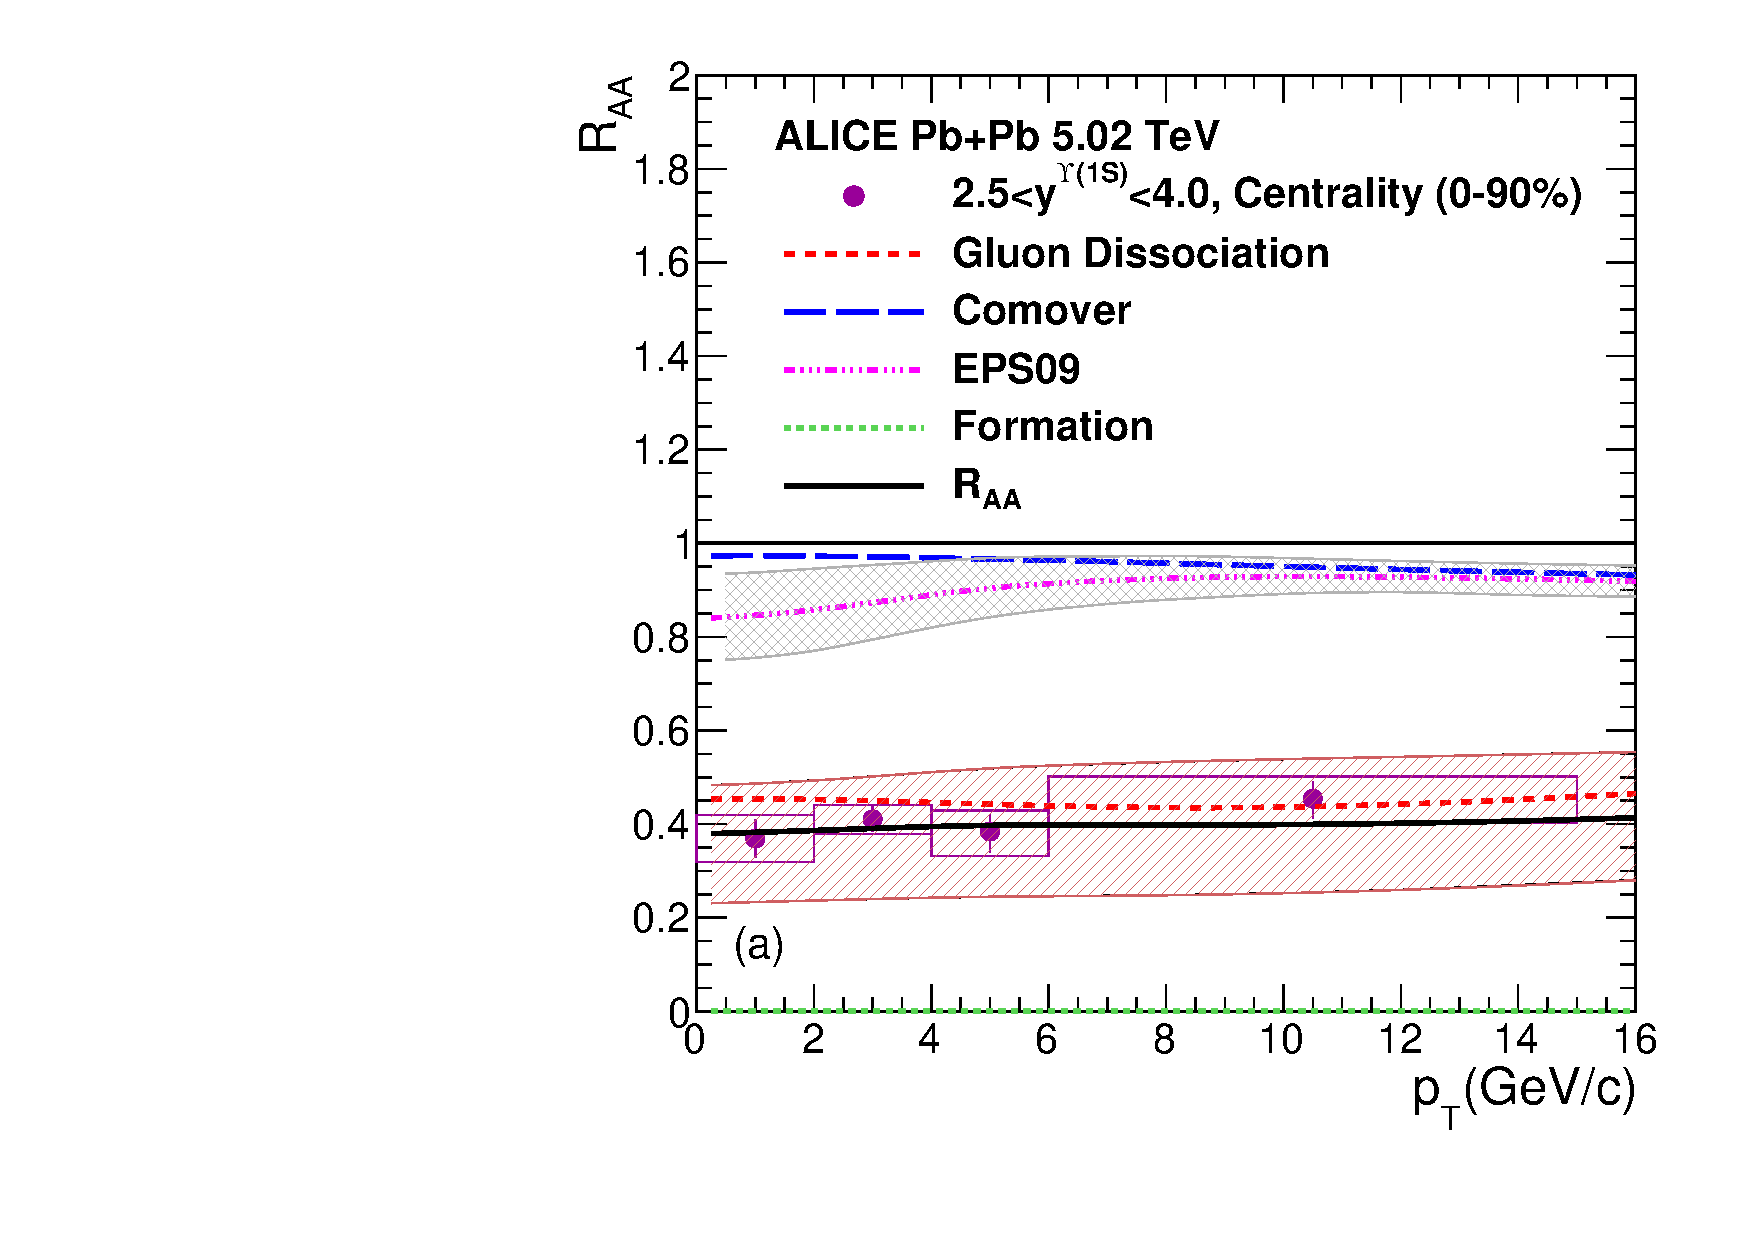
\includegraphics[width=0.49\textwidth]{Figures/Quarkonia_502TeV/Fig8a_ALICE_Y1SRAAPt_Shade.pdf}
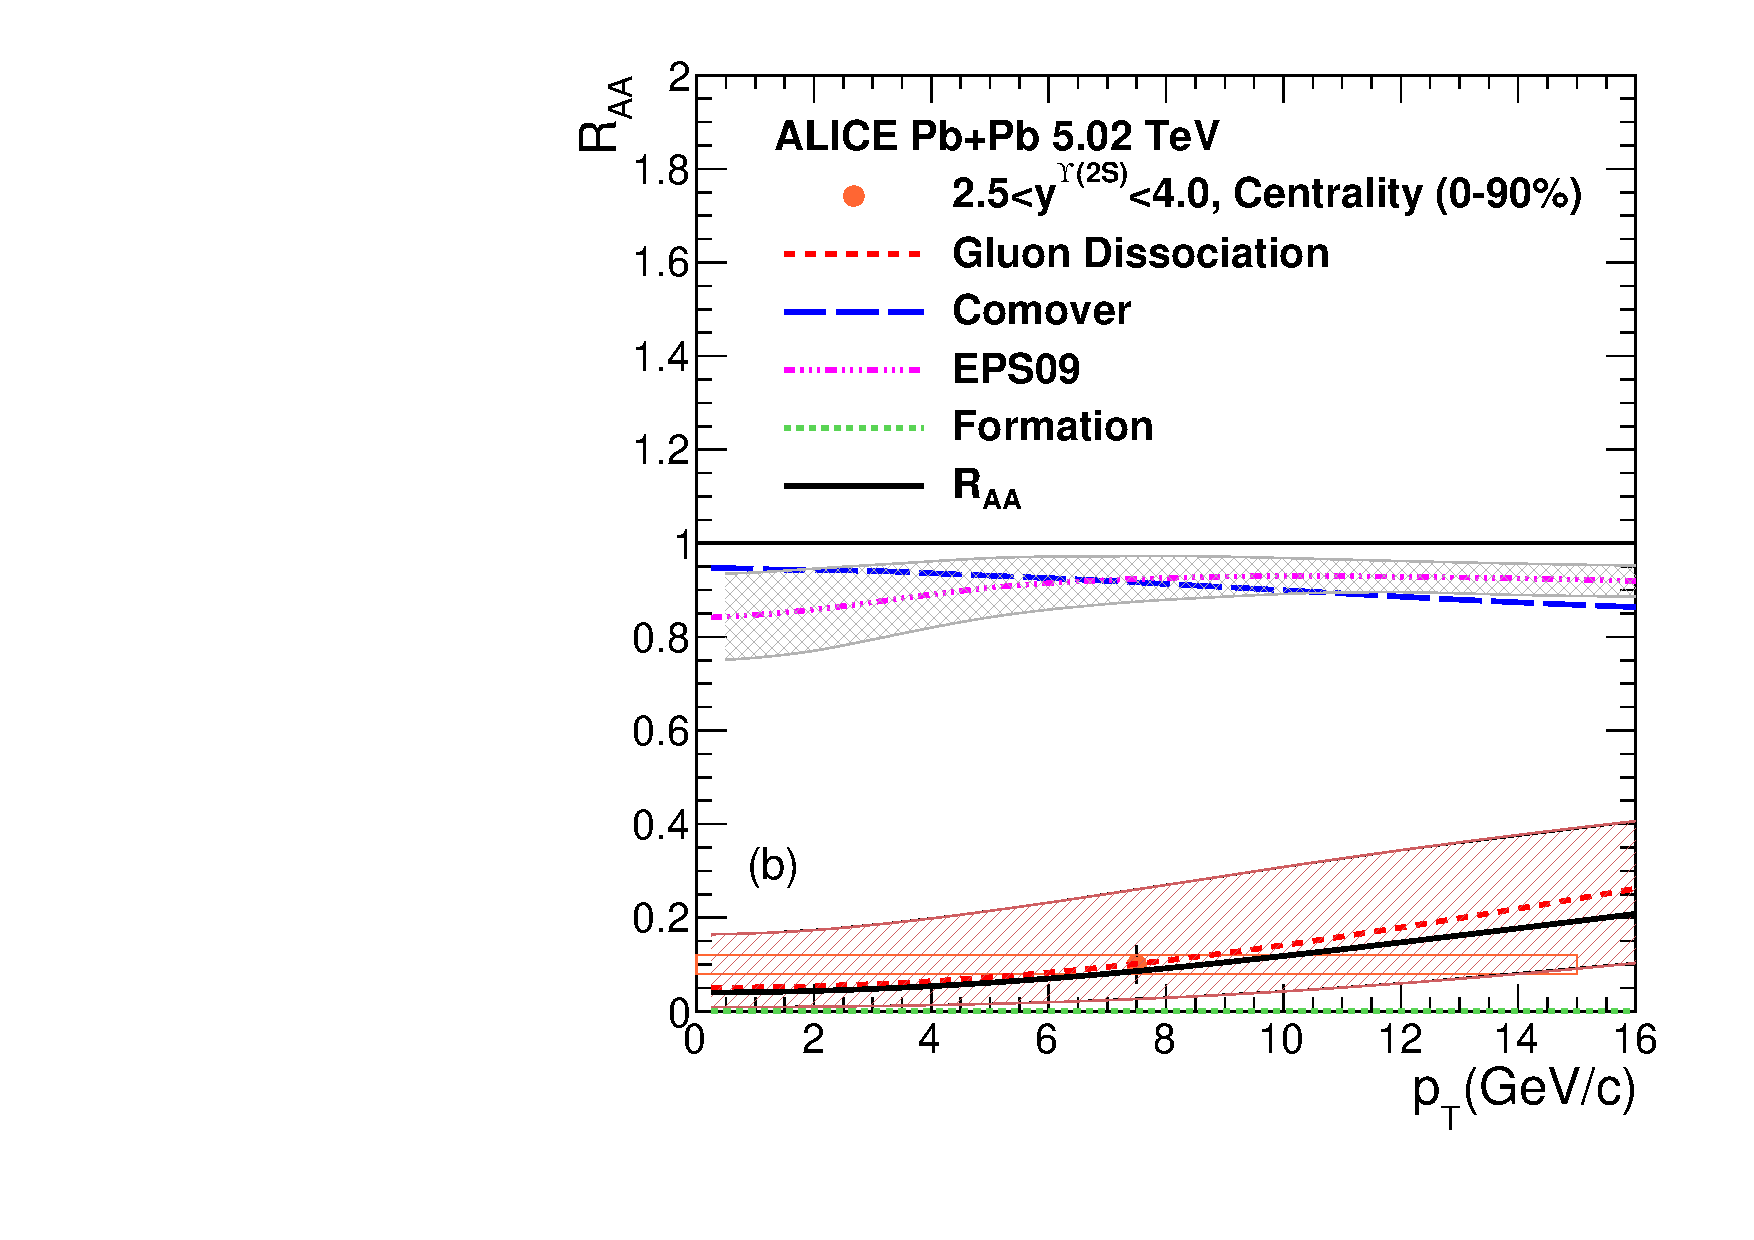
\includegraphics[width=0.49\textwidth]{Figures/Quarkonia_502TeV/Fig8b_ALICE_Y2SRAAPt_Shade.pdf}
\caption{(Color online) Calculated nuclear modification factor ($R_{AA}$) of (a) $\Upsilon$(1S) and 
  (b) $\Upsilon$(2S) as a function of $p_{T}$ in the kinematic range of ALICE detector at LHC ~\cite{ALICE:Y5TeV}.
  The global uncertainty in $R_{AA}$ is shown as a band around the line at 1.
} 
\label{fig:UpsilonRaaPtALICE}
\end{figure}

\begin{figure}
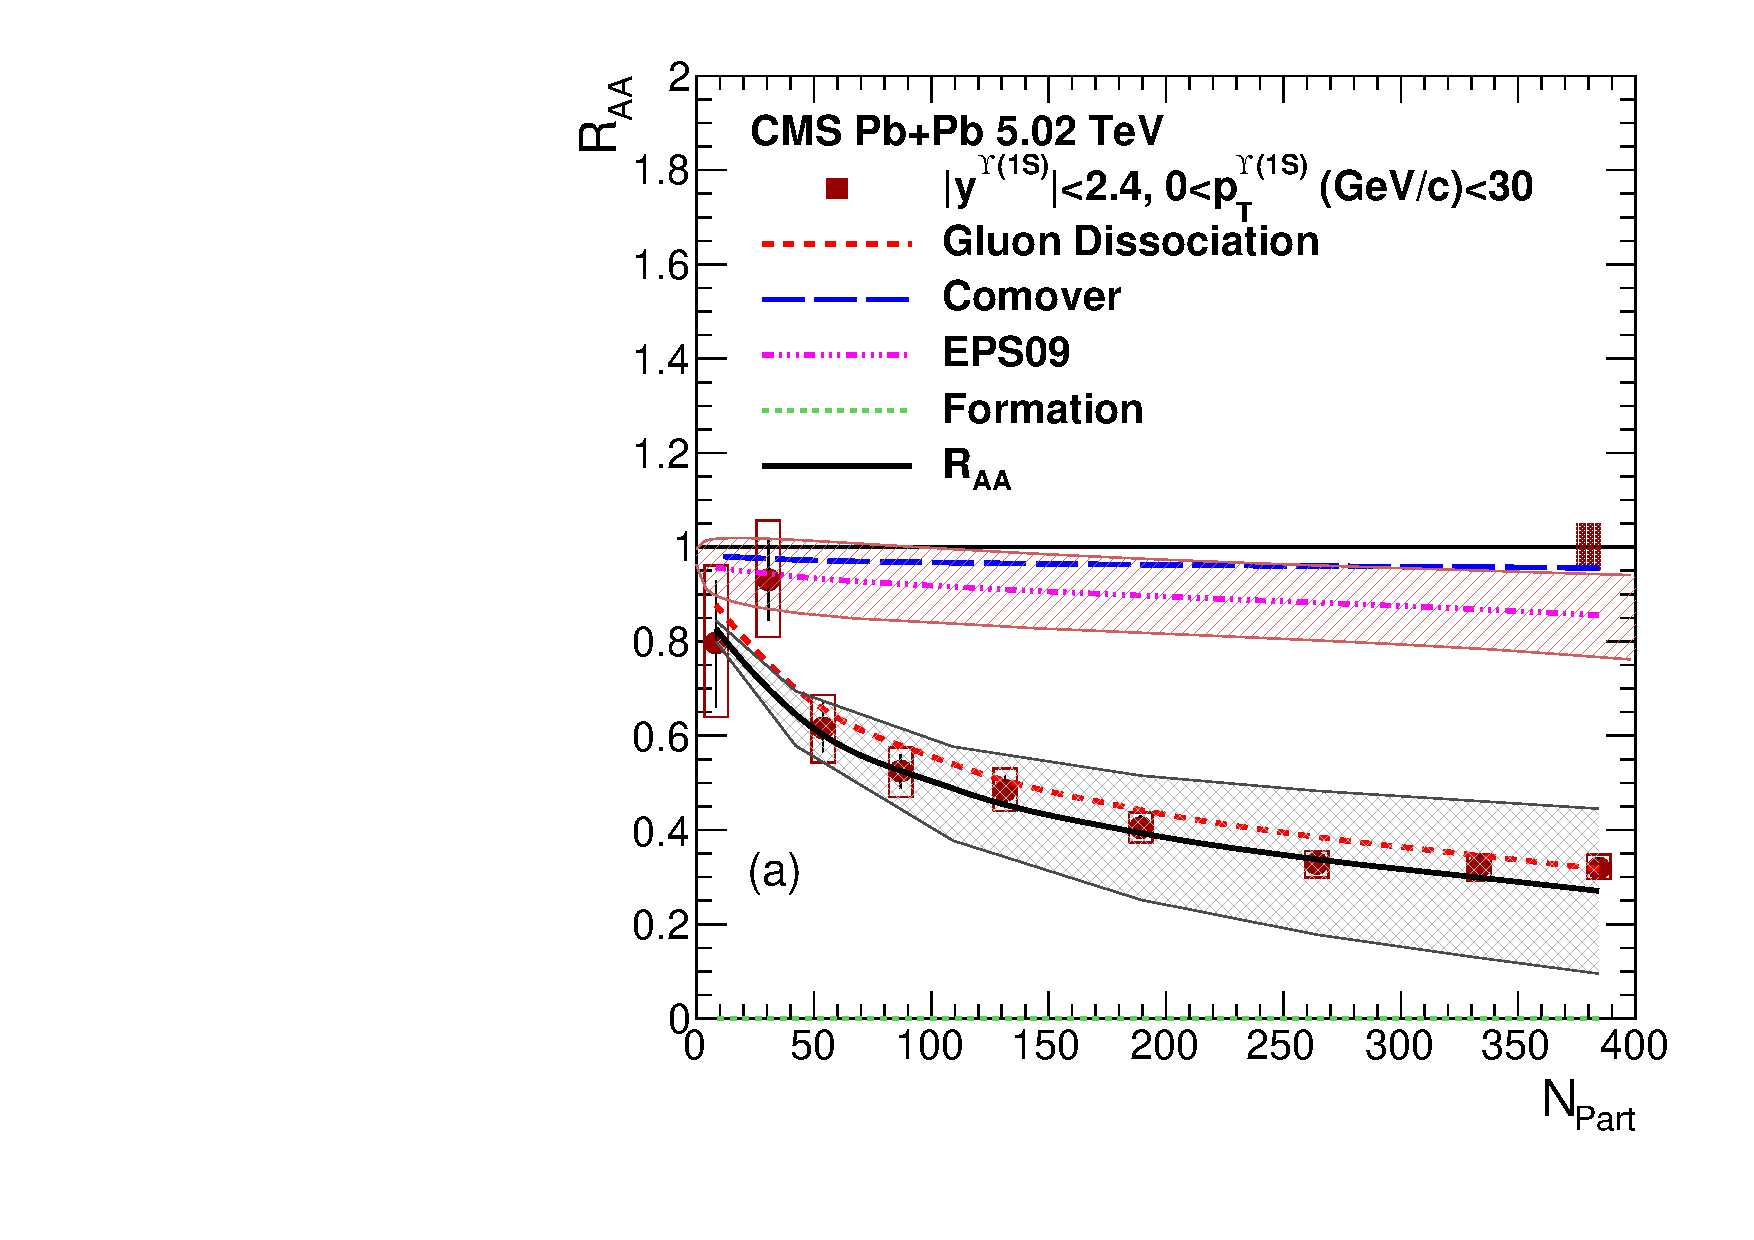
\includegraphics[width=0.49\textwidth]{Figures/Quarkonia_502TeV/Fig9a_CMS_Y1SRAANPart_Shade.pdf}
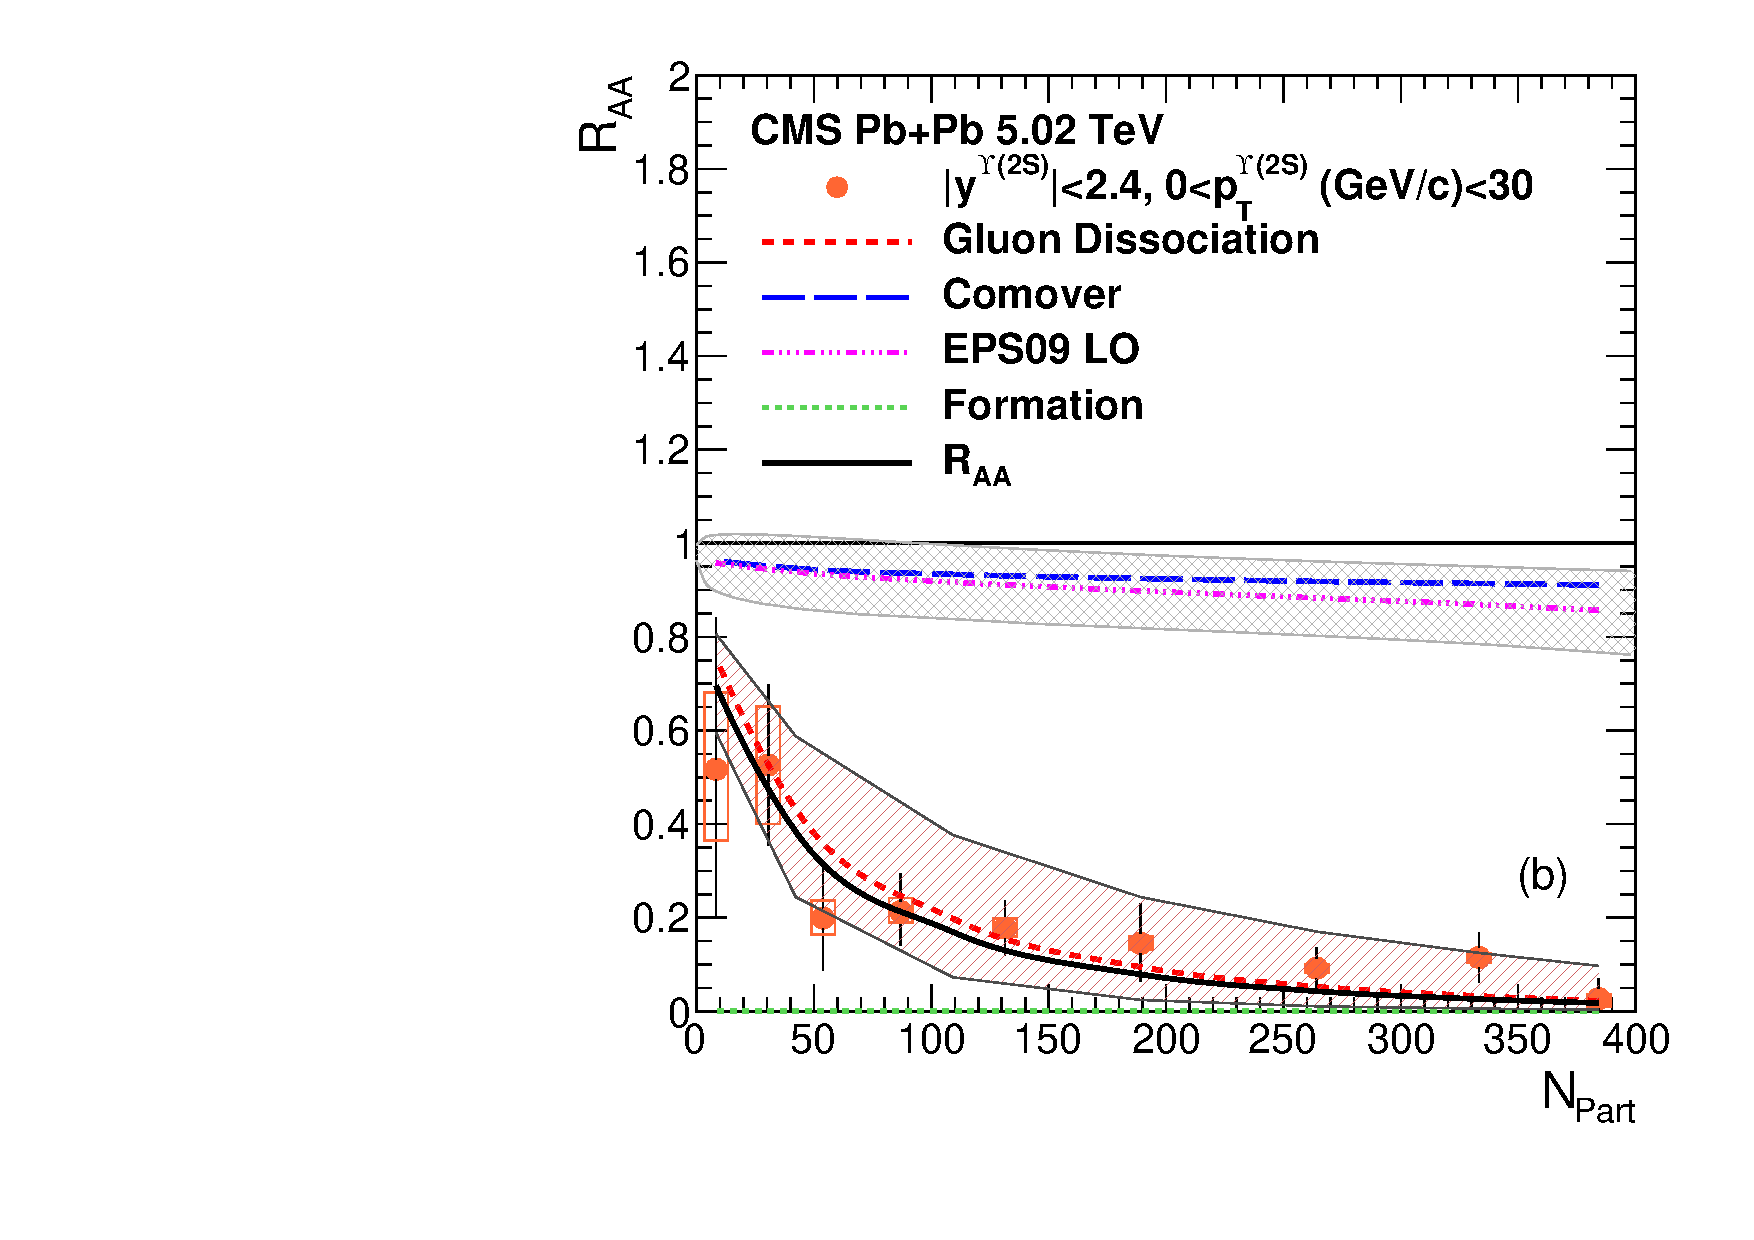
\includegraphics[width=0.49\textwidth]{Figures/Quarkonia_502TeV/Fig9b_CMS_Y2SRAANPart_Shade.pdf}
\caption{(Color online) Calculated nuclear modification factor ($R_{AA}$) of 
  (a) $\Upsilon$(1S) and (b) $\Upsilon$(2S) as a function of centrality of the 
  collisions compared with the CMS measurements~\cite{Sirunyan:2018nsz}.%\cite{CMS:2017ucd}.
  The global uncertainty in $R_{AA}$ is shown as a band around the line at 1.
}
\label{fig:UpsilonRaaNPartCMS}
\end{figure}


Figure~\ref{fig:UpsilonRaaPtCMS}(a) and (b) show the calculations of contributions to
the nuclear modification factor, $R_{AA}$, for the $\Upsilon$(1S) and $\Upsilon$(2S)
respectively as a function of $p_T$ compared with the mid rapidity measurements from
CMS~\cite{Sirunyan:2018nsz}.  
The gluon dissociation mechanism combined with the pion dissociation and shadowing
corrections gives good description of data in mid $p_{T}$ range ($p_{T}\approx$ 5-10 GeV/c)
for both $\Upsilon$(1S) and $\Upsilon$(2S).
The contribution from the regenerated $\Upsilon$s is negligible even at LHC energies.
Our calculations under-predict the suppression observed at the highest measured
$p_{T}$ for $\Upsilon$(1S) and $\Upsilon$(2S) which is similar for the case
of J/$\psi$.
%The feed-down corrections are applied in our calculations following the similar
%procedure as in Refs.~\cite{Abdulsalam:2012bw,Krouppa:2017jlg}. 
%%%%%%%%% insert the feed-down details here
The states $\Upsilon$(1S) and $\Upsilon$(2S) also have
feed-down contributions from decays of higher b$\bar{\rm b}$ bound states.
The nuclear modification factor, $R_{AA}$ is obtained taking into account the feed-down corrections as follows
  \begin{equation}
    R_{AA}^{\Upsilon(3S)} = R_{AA}^{\Upsilon(3S)}\\ %\nonumber
  \end{equation}
  \begin{equation}
    R_{AA}^{\Upsilon(2S)} = f_1 R_{AA}^{\Upsilon(2S)} +  f_2 R_{AA}^{\Upsilon(3S)} \\ %\nonumber
  \end{equation}
   \begin{equation}
    R_{AA}^{\Upsilon(1S)} = g_1 R_{AA}^{\Upsilon(1S)} +  g_2 R_{AA}^{\chi_b(1P)} + g_3 R_{AA}^{\Upsilon(2S)} + g_4 R_{AA}^{\Upsilon(3S)}\\ %\nonumber
  \end{equation}
The factors $f$’s and $g$’s are obtained from CDF measurement~\cite{Affolder:1999wm}.
The values of $g_1$, $g_2$, $g_3$ and $g_4$ are 0.509, 0.27, 0.107
and 0.113 respectively. Here $g_4$ is assumed to be the combined fraction of 
$\Upsilon$(3S) and $\chi_b$(2P).
The values of $f_1$ and $f_2$ are taken as 0.50~\cite{Strickland:2011aa}.


Figure~\ref{fig:UpsilonRaaPtALICE}(a) and (b) show the model 
prediction of the nuclear modification factor, $R_{AA}$, for the $\Upsilon$(1S)
and $\Upsilon$(2S) respectively as a function of $p_T$ in the kinematic range
covered by ALICE detector. The ALICE data~\cite{ALICE:Y5TeV} is well described by our model.

Figure~\ref{fig:UpsilonRaaNPartCMS}(a) depicts the calculated 
centrality dependence of the $\Upsilon$(1S) nuclear
modification factor, along with the midrapidity data from CMS~\cite{Sirunyan:2018nsz}.
Our calculations combined with the pion dissociation and shadowing corrections 
gives very good description of the measured data. Figure~\ref{fig:UpsilonRaaNPartCMS}(b)
shows the same for the $\Upsilon$(2S) along with the midrapidity
CMS measurements. The suppression of the excited $\Upsilon$(2S) states 
is also well described by our model. As stated earlier, the effect of regeneration is
negligible for $\Upsilon$ states. 

Figure~\ref{fig:UpsilonRaaNPartALICE}(a) shows the forward rapidity ALICE
measurement of the $\Upsilon$(1S) nuclear modification factor~\cite{ALICE:Y5TeV}
along with our calculations. The suppression due to thermal gluon dissociation 
describes the measured data after including the comover and shadowing corrections.
Figure~\ref{fig:UpsilonRaaNPartALICE}(b) shows the calculations for the
$\Upsilon$(2S) nuclear modification factor in ALICE detector kinematic range.
The suppression due to thermal gluon dissociation describes the
ALICE measurements after including the comover and shadowing corrections.
















  %%%%%%%%%%%%%%%%%%%%%%%%%%%%%%%%%%%%%%%%%%%%%%%%%%%%%%%%%%%%%%%%%%%%%%%%%%%%%%%%%%%%%%%%
  \subsubsection{Statistical (re) generation models}
  {\color{red} We can include the regenration part from our calculations. These effects are also small.}


%\subsubsection{Non-equilibrium effects on quarkonium suppression}
%\subsubsection{Collisional dissociation of quarkonia from final-state interactions}

\subsubsection{Comover models}

%\section{hadronic comovers}
  The suppression of quarkonia by comoving pions can be calculated by folding the quarkonium-pion
dissociation cross section $\sigma_{\pi Q}$ over thermal pion distributions \cite{Vogt:1988fj}. 
It is expected  that at LHC energies, the comover cross section will be small~\cite{Lourenco:2008sk}.
{\color{black}
The pion-quarkonia cross section is calculated by convoluting the gluon-quarkonia cross section $\sigma_D$
over the gluon distribution inside the pion~\cite{Arleo:2001mp},
\begin{equation}
\sigma_{\pi Q} (p_{\pi}) = {p_+^2 \over 2(p_\pi^2 - m_\pi^2)} \int_0^1 \, dx \, G(x) \, \sigma_D(xp_+/\sqrt {2}),
\end{equation}
where $p_+ = (p_\pi + \sqrt{p_\pi^2-m_\pi^2})/\sqrt{2}$. The gluon distribution, $G(x)$, inside a pion is 
given by the GRV parameterization~\cite{Gluck:1991ey}. 
The pion momentum $p_\pi$ is related to center of mass energy $\sqrt{s}$ of pion-$J/\psi$ system by 
$p_\pi = (s-M_Q^2-m_\pi^2)/(2M_Q)$.}
The dissociation rate $\lambda_{D_{\pi}}$  can be written as
\begin{eqnarray}
  \lambda_{D_{\pi}} \, \rho_{\pi} & = & \frac{g_\pi}{(2\pi)^{3}} \int d^{3}p_{\pi} f_{\pi}(p) \sigma_{\pi Q} (s) v_{\rm rel} (s) \\ \nonumber
                              & = &\frac{g_\pi}{(2\pi)^{3}} \int\,dp_{\pi}\,2\pi p_{\pi}^{2} f_{\pi}(p_{\pi}) \int\,d{\rm cos}\theta\,\sigma_{\pi Q}(s) \, v_{\rm rel}(s) \Theta(s-4m_{D}^{2}),  \\\nonumber
\end{eqnarray}
where $f_{\pi}(p_{\pi},T)$ is the thermal pion distribution. The  pion density $\rho_{\pi}$ is 
\begin{eqnarray}
\rho_\pi =\frac{g_\pi}{(2\pi)^{3}} \int d^3p_{\pi} \, f_{\pi}(p_{\pi}). 
\end{eqnarray}
The survival probability from pion collisions at freeze-out time $\tau_f$ is written as
\begin{equation}
S_\pi(p_T) = \exp \left( {-\int_{\tau_0}^{\tau_f} \,d\tau\,(1-f(\tau)) \lambda_{D_{\pi}}(T,p_T)\,\rho_{\pi}(T)} \right).
\end{equation}
The hadronic fraction (1-$f(\tau)$) is zero in QGP phase.
The probability $S_\pi(p_T)$ multiplies $S(p_T)$ in Eq.~(\ref{raa}).



\subsubsection{Summary of theoretical models for experimental comparison}

{\color{red} We will write the summary for all different type of quarkonia model here.}


\subsection{Experimental overview of Bottomonia results at RHIC and LHC}

%\subsubsection{Proton–proton collisions as a reference for R$_{AA}$ at the LHC}

\subsubsection{$\Upsilon$(nS) R$_{AA}$ at the LHC}

\paragraph{Measurement by CMS, ATLAS and ALICE}

The bottomonia states ($\Upsilon$(nS)) are measured at the LHC with very good statistical
precision~\cite{Chatrchyan:2011pe,Chatrchyan:2012lxa,Abelev:2014nua,Khachatryan:2016xxp}.
The CMS measurements at $\sNN =$2.76 TeV~\cite{Chatrchyan:2011pe,Chatrchyan:2012lxa} reveal
a clear proof of sequential suppression :  $\Upsilon$(2S) and $\Upsilon$(3S) are 
more suppressed relative to the ground state $\Upsilon$(1S).   The individual $\Upsilon$ states are also found to be suppressed in
the PbPb collisions relative to the production in the pp collisions. The $\Upsilon$ nuclear
modification factor, $R_{AA}$, shows a strong dependence on collision centrality but has
weak dependence on $\Upsilon$ meson $\pT$ and rapidity~\cite{Khachatryan:2016xxp}.
The forward rapidity ($2.5 \leq y^{\Upsilon} \leq 4.0$) measurement of the $\Upsilon$ suppression at 
ALICE~\cite{Abelev:2014nua} is found to be consistent with the midrapidity ($|y^{\Upsilon}|\,\leq 2.4$)
measurement of the $\Upsilon$ suppression at the CMS. 
The CMS and ALICE collaborations have carried out the $R_{AA}$ measurement of $\Upsilon$
at $\sNN =$ 5.02 TeV with the Run II LHC PbPb
collisions~\cite{Sirunyan:2017lzi,Sirunyan:2018nsz,ALICE:Y5TeV}.
The CMS experiment measured slightly more amount of $\Upsilon$ suppression at
$\sNN =$ 5.02 TeV~\cite{Sirunyan:2017lzi,Sirunyan:2018nsz} than the suppression at
$\sNN =$ 2.76 TeV~\cite{Khachatryan:2016xxp} while the ALICE experiment observed less
suppression at $\sNN =$ 5.02 TeV than that at $\sNN =$ 2.76 TeV 
in the most central PbPb collisions~\cite{Abelev:2014nua,ALICE:Y5TeV}.





\subsubsection{$\Upsilon$(nS) azimuthal anisotropy at the LHC}

\paragraph{Measurement by CMS and ATLAS}

\subsubsection{$\Upsilon$(nS) R$_{AA}$ at the RHIC}

\paragraph{Measurement by STAR and PHENIX}

\subsubsection{Summary and outlook}

This will include comparison of RHIC and LHC results and then overview.


\section{Conclusions and oulook}





\section*{References}
%\printbibliography %% for biber
\bibliography{BeautyExp}


\end{document}
